%! TeX root = relazione.tex

\documentclass{article}

\usepackage[italian]{babel}

\usepackage{listings}             % Scrivere le linee di comando con lsrlisting
\usepackage{graphicx}     % Centrare i testi con center
\usepackage[colorlinks=true, allcolors=blue]{hyperref}  % Link ipertestuali
\usepackage{amsmath}    % Usato per scrivere in linguaggio matematico

% Set page size and margins
% Replace `letterpaper' with `a4paper' for UK/EU standard size
\usepackage[letterpaper,top=2cm,bottom=2cm,left=3cm,right=3cm,marginparwidth=1.75cm]{geometry}

\title{\textbf{KMEANS}}
\author{\textbf{Programmazione di Sistemi Embedded e Multicore}}
\begin{document}
  \maketitle

  \begin{description}
    \centering
    \item \textbf{Nome}: Rideewitage Lachitha Sangeeth 
    \item \textbf{Cognome}: Perera \textbf{Matricola}: 2042904
  \end{description}

  \section{Introduzione}

  Per la parellizzazione del codice sequenziale di KMEANS, sono stati utilizzati due metodi, uno che consiste l'utilizzo di \textbf{OpenMP} insieme a \textbf{OpenMPI},
  e l'altro metodo che utilizza interamente \textbf{CUDA}.
  Prima di analizzare i codici parallelizzati, è necessario capire il funzionamento del codice sequenziale di KMEANS, in quanto sono state apportate delle leggere
  modifiche per il funzionamento dei test.

  
  La prima modifica effettuata al codice sequenziale è stata l'aggiunta di un paramentro in input, che permette di salvare in un file csv il computation time, il quale
  verrà utilizzato per il calcolo della media dei tempi e confrontato con le altre versioni, per la realizzazione di ciò è stata aggiunta anche una funzione che scrive il computation
  time nel file specificato in input [\ref{Write}]. 
  I file contententi i computation times sono salvati in una directory specifica, 
  ovvero: 
  \begin{center}    
    \verb|comp_time/{versione}/comp_time{grandezza_test}.csv|.
  \end{center}
  Oltre a questo, per il corretto funzionamento di tutte le versioni, è stata 
  apportata anche un modifica per quanto riguarda la funzione \verb|eucledianDistance| [\ref{Eucledian}].
  \begin{figure}[ht]
    \hspace{-3cm} % Sposta la figura più a sinistra
    \centering
    \begin{minipage}{0.4\textwidth}
        \centering
        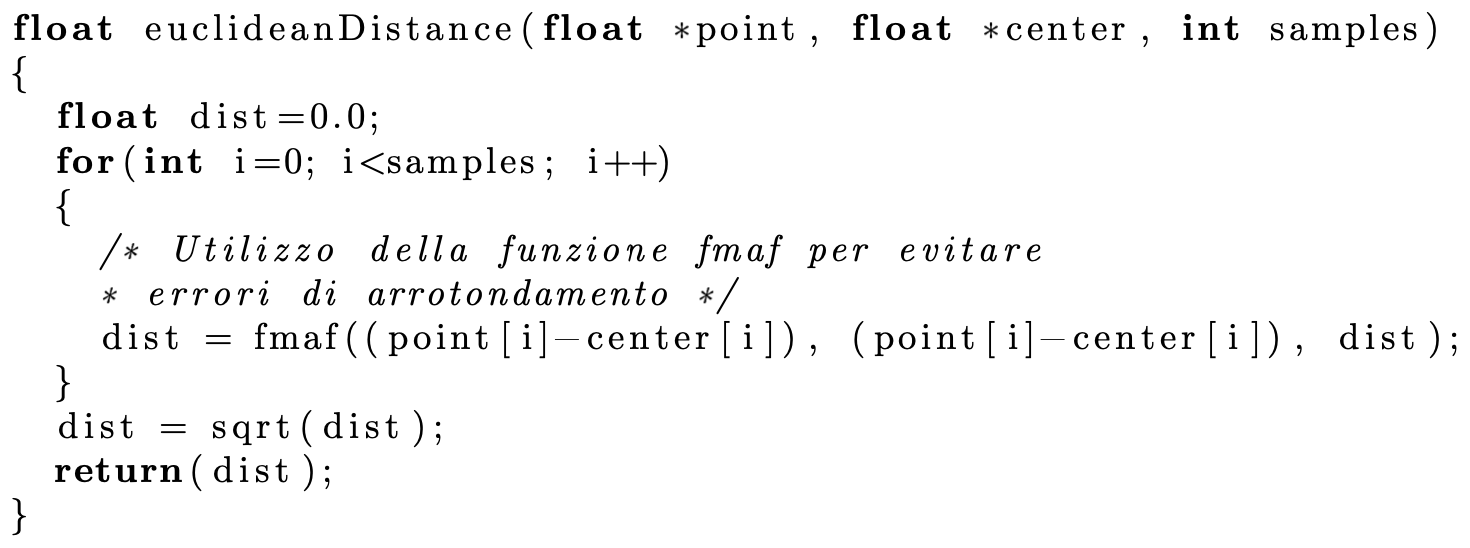
\includegraphics[width=1.5\linewidth]{./Eucledian.png}
        \caption{\textbf{EucledianDistance}}
        \label{Eucledian}
    \end{minipage}
    \hspace{4cm} % Sposta la figura più a sinistra
    \begin{minipage}{0.4\textwidth}
      \centering
      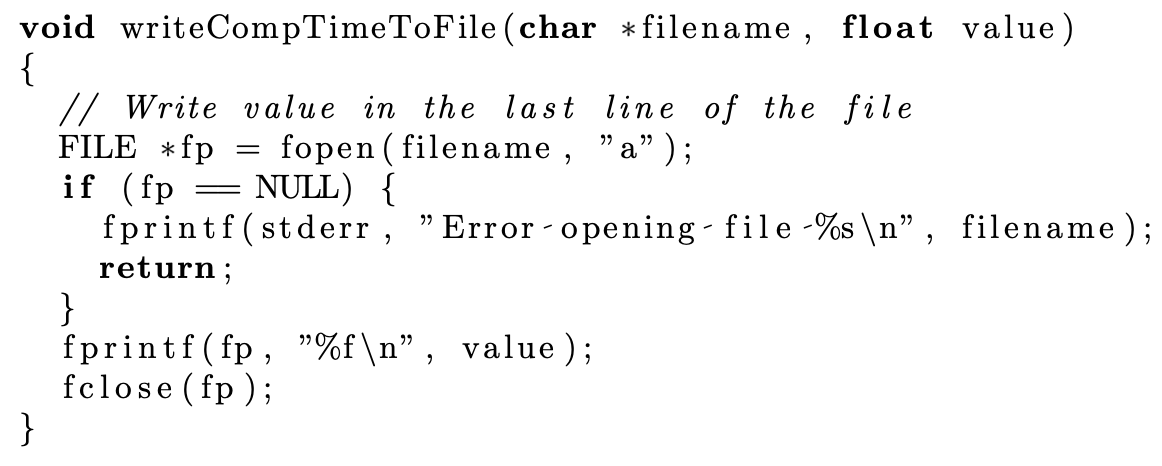
\includegraphics[width=1.4\linewidth]{./Write-Comp.png}
      \caption{\textbf{Write-Comp}}
      \label{Write}
    \end{minipage}
  \end{figure}

  Come è possibile notare dal codice, è stata utilizzata la funzione \verb|fmaf| per evitare possibilie errori
  di arrotondamento; questa modifica è stata apportata in tutte le versioni del codice, questo per fare 
  in modo che la versione ci CUDA non desse output differenti dal sequenziale, in quanto utilizzando la GPU per i calcoli 
  gli arrotondamenti vengono eseguiti in modo diverso rispetto alla CPU. Con l'utlizzo di fmaf, si riduce il numero di arrotondamenti,
  dimnuendo la possibilità di errori.
  \begin{center}
    \rule{6cm}{1pt}
  \end{center}
  Per quanto riguarda il resto del codice, per parallelizzare il codice sequenziale di KMEANS è stato diviso il ciclo \verb|do - while| i tre parti
  fondaemntali, ovvero: 
  \begin{enumerate}
    \item Il reset delle variabili utilizzate ad ogni iterazione [\ref{f_section}]
    \item Il calcolo dei nuovi centroidi e l'assegnazione dei punti ai cluster [\ref{s_section}]
    \item Il calcolo della distanza massima tra i centroidi vecchi e quelli nuovi, per il controllo della threshold impostata dai parametri in input [\ref{t_section}]
  \end{enumerate}
  
  \begin{figure}[ht]
    \centering
    \begin{minipage}{0.4\textwidth}
        \centering
        \caption{\textbf{First section}}
        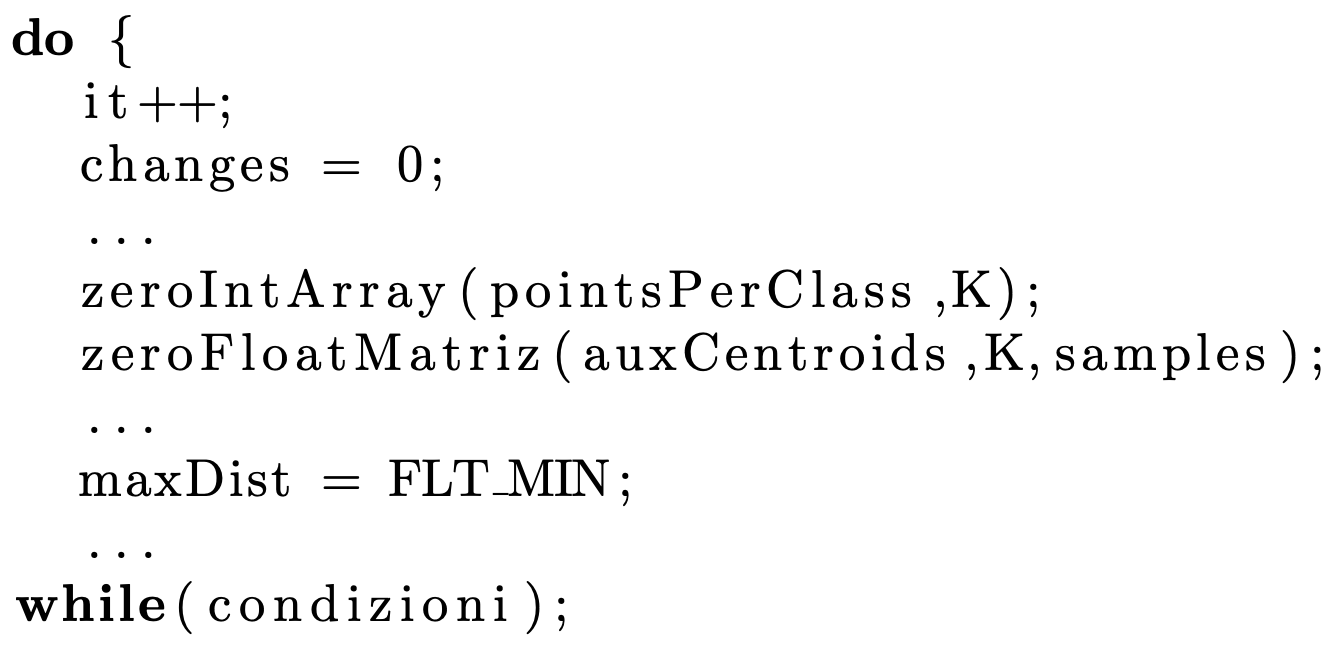
\includegraphics[width=\linewidth]{./First-section.png}
        \label{f_section}
    \end{minipage}
    \begin{minipage}{0.5\textwidth}
        \centering
        \caption{\textbf{Second section}}
        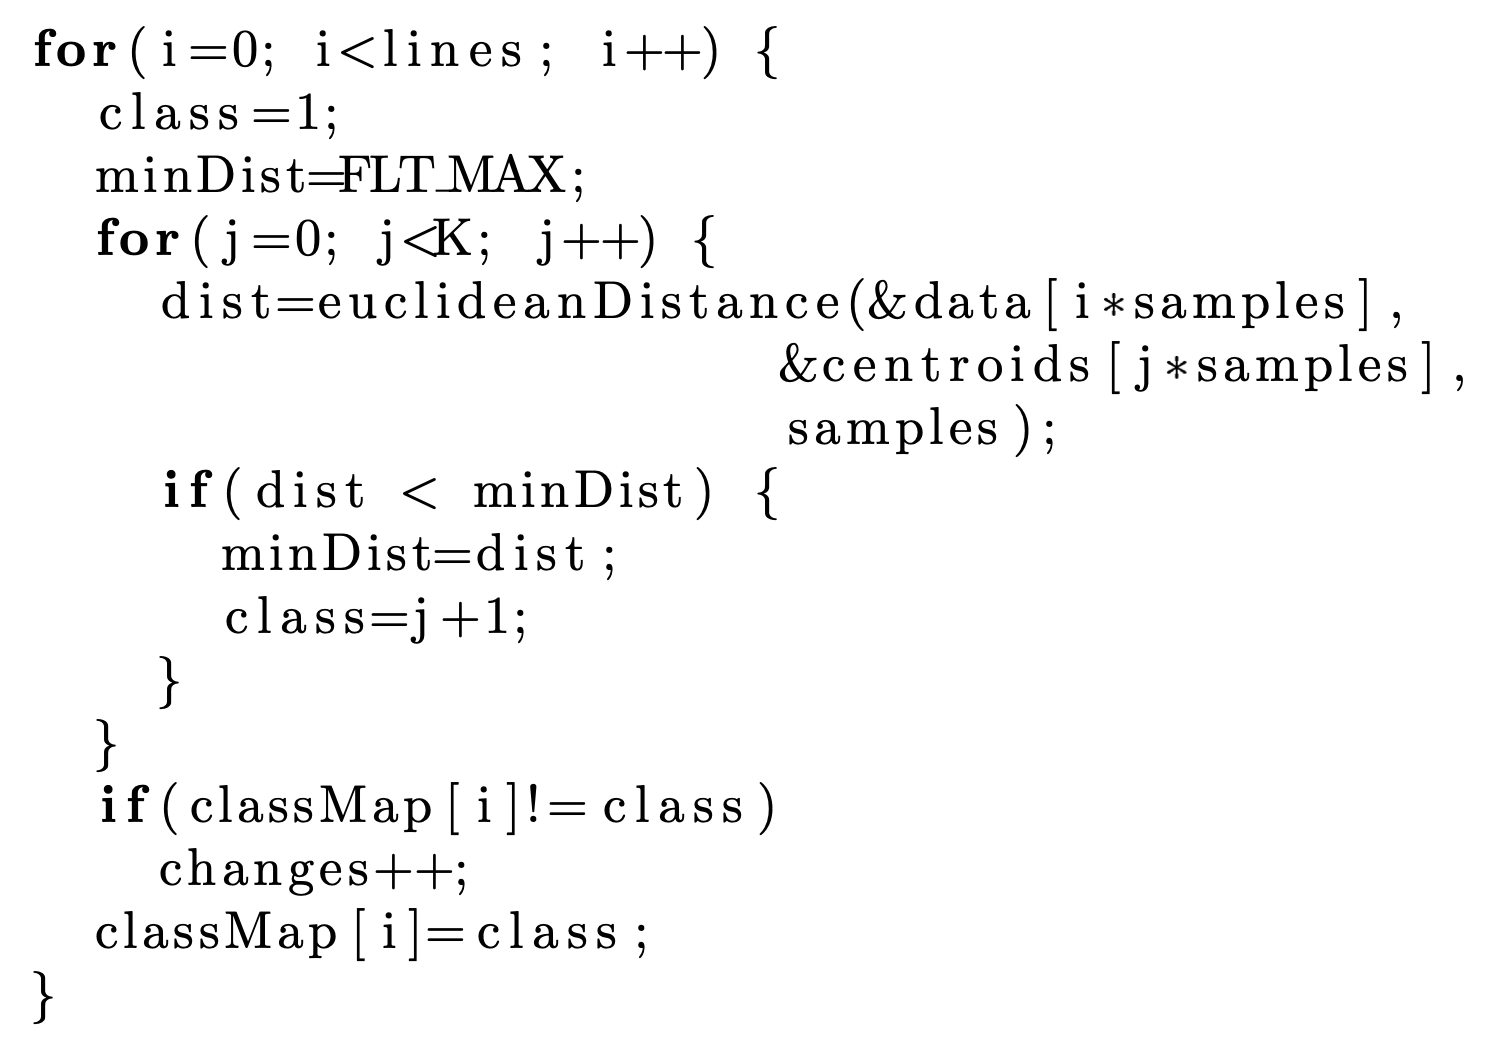
\includegraphics[width=\linewidth]{./Second-section.png}
        \label{s_section}
    \end{minipage}
    \begin{minipage}{0.65\textwidth}
        \centering
        \caption{\textbf{Third section}}
        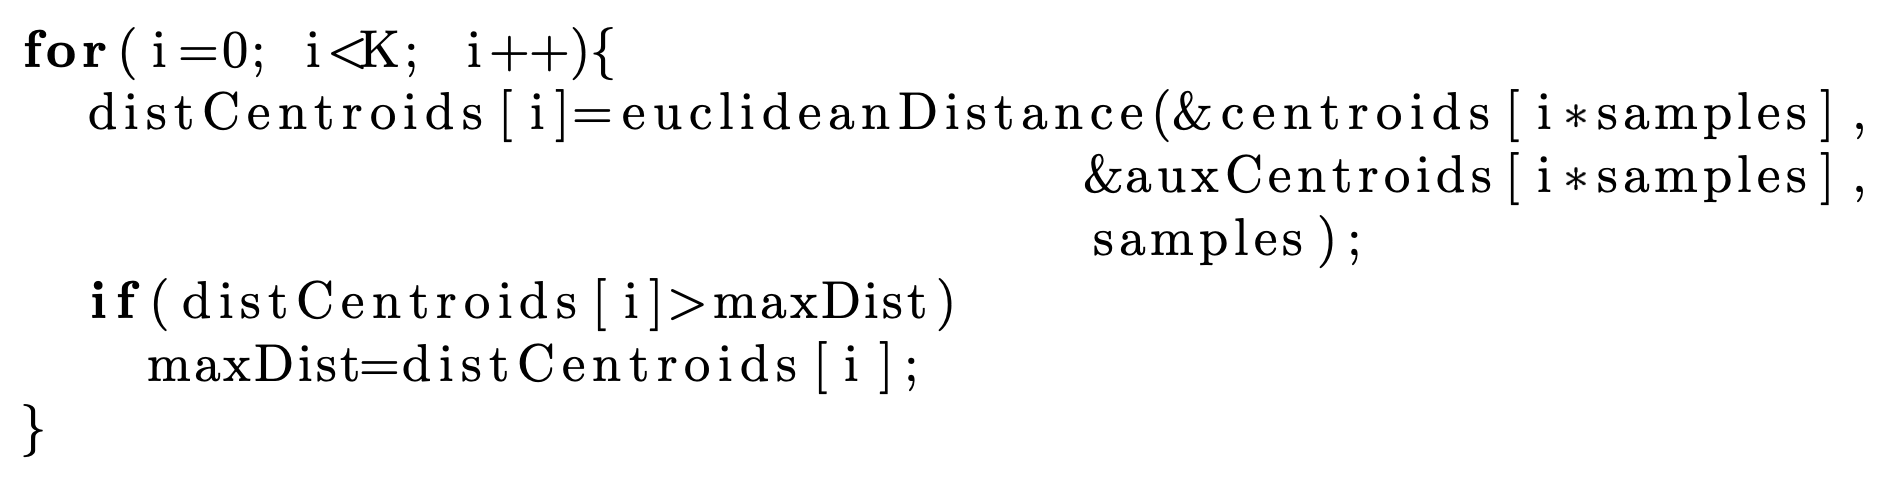
\includegraphics[width=\linewidth]{./Third-section.png}
        \label{t_section}
    \end{minipage}
  \end{figure}
  La parallelizzazione della versione sequenziale, è stata effettuata cercando di parallellizzare le 3 parti appena descritte.
  Oltre a queste parti, è importante anche capire la gestioni dei dati all'interno di ogni iterazione, le variabili 
  che sono state tenute con maggior considerazione durante la parallelizzazione sono: \verb|pointPerClass|, \verb|auxCentroids|,
  \verb|classMap|, \verb|centroids|, \verb|maxDist|, \verb|classMap|.
  \begin{center}
    \rule{6cm}{1pt}
  \end{center}
  Per quanto riguarda \verb|pointPerClass| e \verb|auxCentroids| sono utilizzate per il calcolo dei nuovi centroidi, che è una sezione 
  del codice che non è stata trattata precedentemente, in quanto è stata poi accorpata con la seconda e la terza sezione. In quanto la prima parte 
  del calcolo viene effettuata su un ciclo che itera sul numero di linee (come la seconda sezione), mentre la seconda parte del calcolo viene effettuata 
  su un ciclo che itera sul numero di cluster (come la terza sezione).
  
  La variabile \verb|classMap| è un array lungo quanto le linee presenti nei file di input, ogni elemento di tale array segna a quale cluster viene assegnata 
  la linea che corrisponde a quell'indice (se \verb|classMap[10] = 5|, allora la linea 10 del file di input viene assegnata al cluster 5). Il contenuto di questa variabile 
  viene poi trascritta con la funzione \verb|writeResult(filename)| sul file passato in input (specificata negli argomenti utilizzando il seguente path:
  \begin{center}
    \verb|output_files/{versione}/output{grandezza_test}.txt|).
  \end{center}
  Invece, la variabile \verb|centroids| rappresenti i centroidi attuali, i quali all'inizio vengono generati randomicamente, in seguito, dopo la prima iterazione del ciclo
  \verb|do - while| viene sovrascritto da \verb|auxCentroids| controllando che la distanza massima di cambiamento, ovvero \verb|maxDist|, sia minore della massima distanza specificata
  negli argomenti.

  \subsection{Check validity and Testing script}

  Per quanto riguarda l'esecuzione dei test per le varie versioni, sono state create degli script python che eseguissero la formattazzione dei file \verb|.slurm| e 
  subito dopo viene eseguito lo sbatch del file. Per avere una media più precisa ogni versione ha eseguito ciascun input file 25 volte, per ogni test i vari parametri passati in input, come il numero di cluster ecc... sono le seguenti:
  \begin{center}
    \verb|./KMEANS_vers file.inp 40 100 1 0.0001 output.txt comp_time.csv|
  \end{center}
  \begin{center}
    \small Number of cluster = 40; Number of iterations = 100; Number of changes = 1; Threshold = 0.0001
  \end{center}
  Dopo l'esecuzione dei vari test (che in ordine di pesantezza seguono il seguente ordine: \textbf{2D2, 10D, 2D, 20D, 100D, 100D2, 200K, 400K, 800K, 1000K}) , con le varie versioni, 
  vengono generati i vari plot per la rappresentazione grafica dello speedup e dell'efficenza dei vari test con i vari file.
  
  Tuttavia, dato che alcuni test file (come il test input2D2.inp) sono molto leggeri, e con pochi dati da elaborare, sono stati creati dei file di test con uno script python, per avere una mole di dati abbastanza grande per 
  avere più parametri di valutazione per quanto riguardano i tempi di esecuzione, l'efficenza e lo speedup. Di conseguenza per la generazione dei test, sono stati creati dei file di 100 dimensioni con: 200K, 400K, 800K e 1000K linee; ed 
  ogni numero è in un range che va da -100 a 100.

  Dopo che una versione ha finito di eseguire ogni test con i vari file di input, vengono salvati le varie medie 
  in un file come menzionato precedentemente, e vengono salvati in una directory specifica per ogni versione, in modo tale da non avere confusione tra i vari file. Ogni file ha la formattazione \verb|.csv| con il seguente 
  header:
  \begin{center}
    \verb| Number of Process, Number of Thread, AvgTime Test 2D2, ..., AvgTime Test 100D_1000K |   
  \end{center}
  \begin{center}
    \small *Nel caso del sequenziale e di CUDA non abbiamo le colonne Number of Process e Number of Thread.
  \end{center}

  \section{CUDA Version}

  Per la versione CUDA sono state implementate due funzioni kernel, che rappresentato due delle sezioni spiegate nell'introduzione (Figure: \ref{s_section} e \ref{t_section}). Per ogni chiamata ad una funzione cuda è stata usata \verb|CHECK_CUDA_CALL| per verificare se la funzione passata in input ha generato un errore.
  Come prima modifica, sono state aggiunte nella sezione di allocazione della memoria le funzioni \verb|cudaMalloc| e \verb|cudaMemcpy| per l'allocazione della memoria sulla GPU e il trasferimento dei dati dalla CPU alla GPU per ogni
  variabile utilizzata all'interno delle funzioni kernel. Per l'utilizzo di dati sulla GPU non è stata utilizzata la shared memory, quindi i dati sono stati semplicemente spostati sulla \textbf{VRAM} della GPU, quindi sono salvati sulla \textbf{Global Memory} essendo la più capiente, utile 
  per salvare i dati in quanto sui test più pesanti si ha una grande quantità di dati. Viene anche utilizzata 
  la memoria \textbf{costant} in quanto alcune variabili non vengono modificate e ogni core ha bisogno di accedere a tale dato in sola lettura, in particolare le variabili definite \verb|__costant__| sono: \verb|d_samples|; \verb|d_K|; \verb|d_lines|.
  
  In seguito all'allocazione della memoria e allo spostamento delle variabili, e prima del ciclo \verb|do| - \verb|while|, 
  vengono impostati le dimensioni di ogni blocco e i thread per blocco in base al numero di linee (determinato dal file di input) e cluster (determinato dal parametro passato in input).
  \begin{lstlisting}[language=C]
    dim3 blockSize(thread_per_block);
    dim3 numBlocks(ceil(static_cast<double>(lines) / blockSize.x));

    dim3 blockSize_K(thread_per_block_K);
    dim3 numBlocks2(ceil(static_cast<double>(K) / blockSize.x));
  \end{lstlisting}
  Come si nota viene utilizzata la funzione \verb|ceil()| in modo che vengano creati un numero di blocchi che raggruppano in modo equo i dati da elaborare, senza scartare dati.
  \subsection{Kernel Functions}
  All'interno del ciclo \verb|do| - \verb|while| vengono inzialmente reimpostate (attraverso la funzione \verb|cudaMemset|) le seguenti variabili: \verb|d_changes|, \verb|d_maxDist|, \verb|d_pointPerClass|, \verb|d_auxCentroids|.
  Inseguito al reset delle variabili vengono chiamati i due kernel. 
  \begin{center}
    \rule{2.5cm}{1pt} \makebox{\texttt{First Kernel Function}} \rule{2.5cm}{1pt}
  \end{center}
  Il primo definito nel seguente modo:
  \begin{enumerate}
    \item Segnatura della funzione:
      \begin{lstlisting}[language=C, xleftmargin=-5em]
        __global__ void assign_centroids(float* d_data, float* d_centroids, 
                        int* d_classMap, int* d_changes, 
                        int* d_pointsPerClass, float* d_auxCentroids)
      \end{lstlisting}
      La funzione viene utilizzata per assegnare ogni punto del file in input al cluster più vicino, e calcolare il numero di punti per ogni cluster e aumenta 
      il numero di cambiamenti per iterazione (ricordiamo che il numero di cambiamenti viene resettato ad ogni iterazione del ciclo) se un punto cambia di cluster. Inseguito
      inizia il calcolo dei nuovi centroidi, che conclude con il secondo kernel.
    \item Inizalmente la funzione calcola l'indice del thread e controlla se il thread è minore del numero di linee:
      \begin{lstlisting}[language=C, xleftmargin=-5em]
        int id = (blockIdx.x * blockDim.x) + threadIdx.x;
        if (id < d_lines)
      \end{lstlisting}
    \item All'interno dell'\verb|if| viene eseguita la seconda sezione [\ref{s_section}], lavorando con le variabili che si trovano nella GPU, spostati precedentemente dalla CPU nella sezione 
      dell'allocazione della memoria, e viene anche accorpata la prima parte del calcolo dei nuovi centroidi:
      \begin{lstlisting}[language=C, xleftmargin=-5em]
        d_classMap[id] = vclass;

        atomicAdd(&d_pointsPerClass[vclass-1], 1);
        for(int j=0; j<d_samples; j++){
            atomicAdd(&d_auxCentroids[(vclass-1)*d_samples+j], 
                    d_data[id*d_samples+j]);
        }
      \end{lstlisting}
      Possiamo inoltre notare l'utilizzo della funzione \verb|atomicAdd| in modo tale da non avere problemi di \textbf{race condition}, ovvero che più thread aggiornino in modo concorrente la stessa variabile.
  \end{enumerate}

  Durante i test, i thread per blocco di questo kernel sono stati impostati con 256, 512 e 1024 thread, per verificare il numero di thread per blocco ideale per questo kernel, in quanto essendo un kernel che lavora su un numero di linee molto alto, 
  bisogna fare in modo che di massimizzare l'utlizzo degli SM della GPU, per avere dei buoni tempi di esecuzione.
  \begin{center}
    \rule{2.5cm}{1pt} \makebox{\texttt{Second Kernel Function}} \rule{2.5cm}{1pt}
  \end{center}
  Per quanto riguarda la seconda funzione, è definita nel seguente modo:
  \begin{enumerate}
    \item Segnatura della funzione:
      \begin{lstlisting}[language=C, xleftmargin=-5em]
        __global__ void max_step(float* d_auxCentroids, int* d_pointsPerClass, 
                        float* d_centroids, float* d_maxDist,
                        float* d_distCentroids)
      \end{lstlisting}
      La funzione viene utilizzata per il calcolo della distanza massima tra i nuovi e i vecchi centroidi, per controllare se la treshold impostata è stata superata. Nel caso viene superata il programma 
      si interrompe. I parametri presi in input sono: \verb|d_auxCentroids| che contiene i centroidi calcolati nella itreazione corrente, \verb|d_pointsPerClass| che contiene il numero di punti per ogni cluster, 
      \verb|d_centroids| che contiene i centroidi attuali, \verb|d_maxDist| che contiene la distanza massima tra i centroidi e \verb|d_distCentroids| che contiene la distanza tra i vecchi e nuovi centroidi.
    \item Come per la prima funzione kernel viene calcolato l'indice del thread controllando se rientra nel numero di cluster totali, impostati con i parametri presi in input.
      \begin{lstlisting}[language=C, xleftmargin=-5em]
        int id = (blockIdx.x * blockDim.x) + threadIdx.x;
        if (id < d_K)
      \end{lstlisting}
    \item All'interno dell'if vengono inizialmente calcolati i nuovi centroidi:
      \begin{lstlisting}[language=C, xleftmargin=-5em]
        for(int j=0; j<d_samples; j++){
            d_auxCentroids[id*d_samples+j] /= d_pointsPerClass[id];
        }
      \end{lstlisting}
    \item Dopo il calcolo dei nuovi centroidi, viene controla la distanza tra i vecchi centroidi e i nuovi, salvando la distanza massima per il controlla con la threshold:
      \begin{lstlisting}[language=C, xleftmargin=-5em]
        d_distCentroids[id]=d_euclideanDistance(&d_centroids[id*d_samples], 
                                        &d_auxCentroids[id*d_samples], 
                                        d_samples);
        if(d_distCentroids[id]>*d_maxDist)
          *d_maxDist = d_distCentroids[id];
      \end{lstlisting}
  \end{enumerate}
  Per quanto riguarda questo kernel il numero di thread per blocco assegnati è di 64 thread per blocco, in quanto questo kernel si incentra nel parallelizzare un porzione di codice che itera sul numero di cluster, che per tutti i test eseguiti il numero 
  di cluster è stata di 40, di conseguenza, a differenza del primo kernel, è stato scelto un numero di thread per blocco in grado di coprire il numero di cluster.
  \subsection{Testing, speedup and difference with sequential}
  Per quanto riguarda la fase di testing del programma, come accennato precedentemente, sono stati usati degli script in python per eseguire i vari test con i vari file di input, calcolando la media dei tempi per ogni test.
  Ogni test prende in input i seguenti parametri:
  \begin{center}
    \small\verb|Number of cluster = 40, Number of iterations = 100, Number of changes = 1, Treshold = 0.0001|
  \end{center}
  Da considerare anche che i vari test, sono stati effettuati cambiando il numero di thread per blocco, solo per il primo kernel, in quanto essendo quello più pesante, sia da lanciare che da eseguire, ha maggior impatto sulle prestazioni, di conseguenza, il numero 
  di thread per blocco del secondo kernel rimane invariato su 64 thread, mentre per il primo kernel sono stati eseguiti i test con 256, 512 e 1024 thread per blocco.
  
  Di seguito sono riportati i grafici dei tempi sia della versione \textbf{CUDA} con 512 thread per blocco confrontati con quelli della versione sequenziale; il grafico è stato diviso in due parti, uno in cui vengono confrontati i test più leggeri, l'altro in cui vengono confrontati i 
  test più pesanti.
  
  \begin{center}
    \rule{2.5cm}{1pt} \makebox{\texttt{Difference with sequential}} \rule{2.5cm}{1pt}
  \end{center}
  \begin{figure}[ht]
    \centering
    \begin{minipage}{0.45\textwidth}
      \centering 
      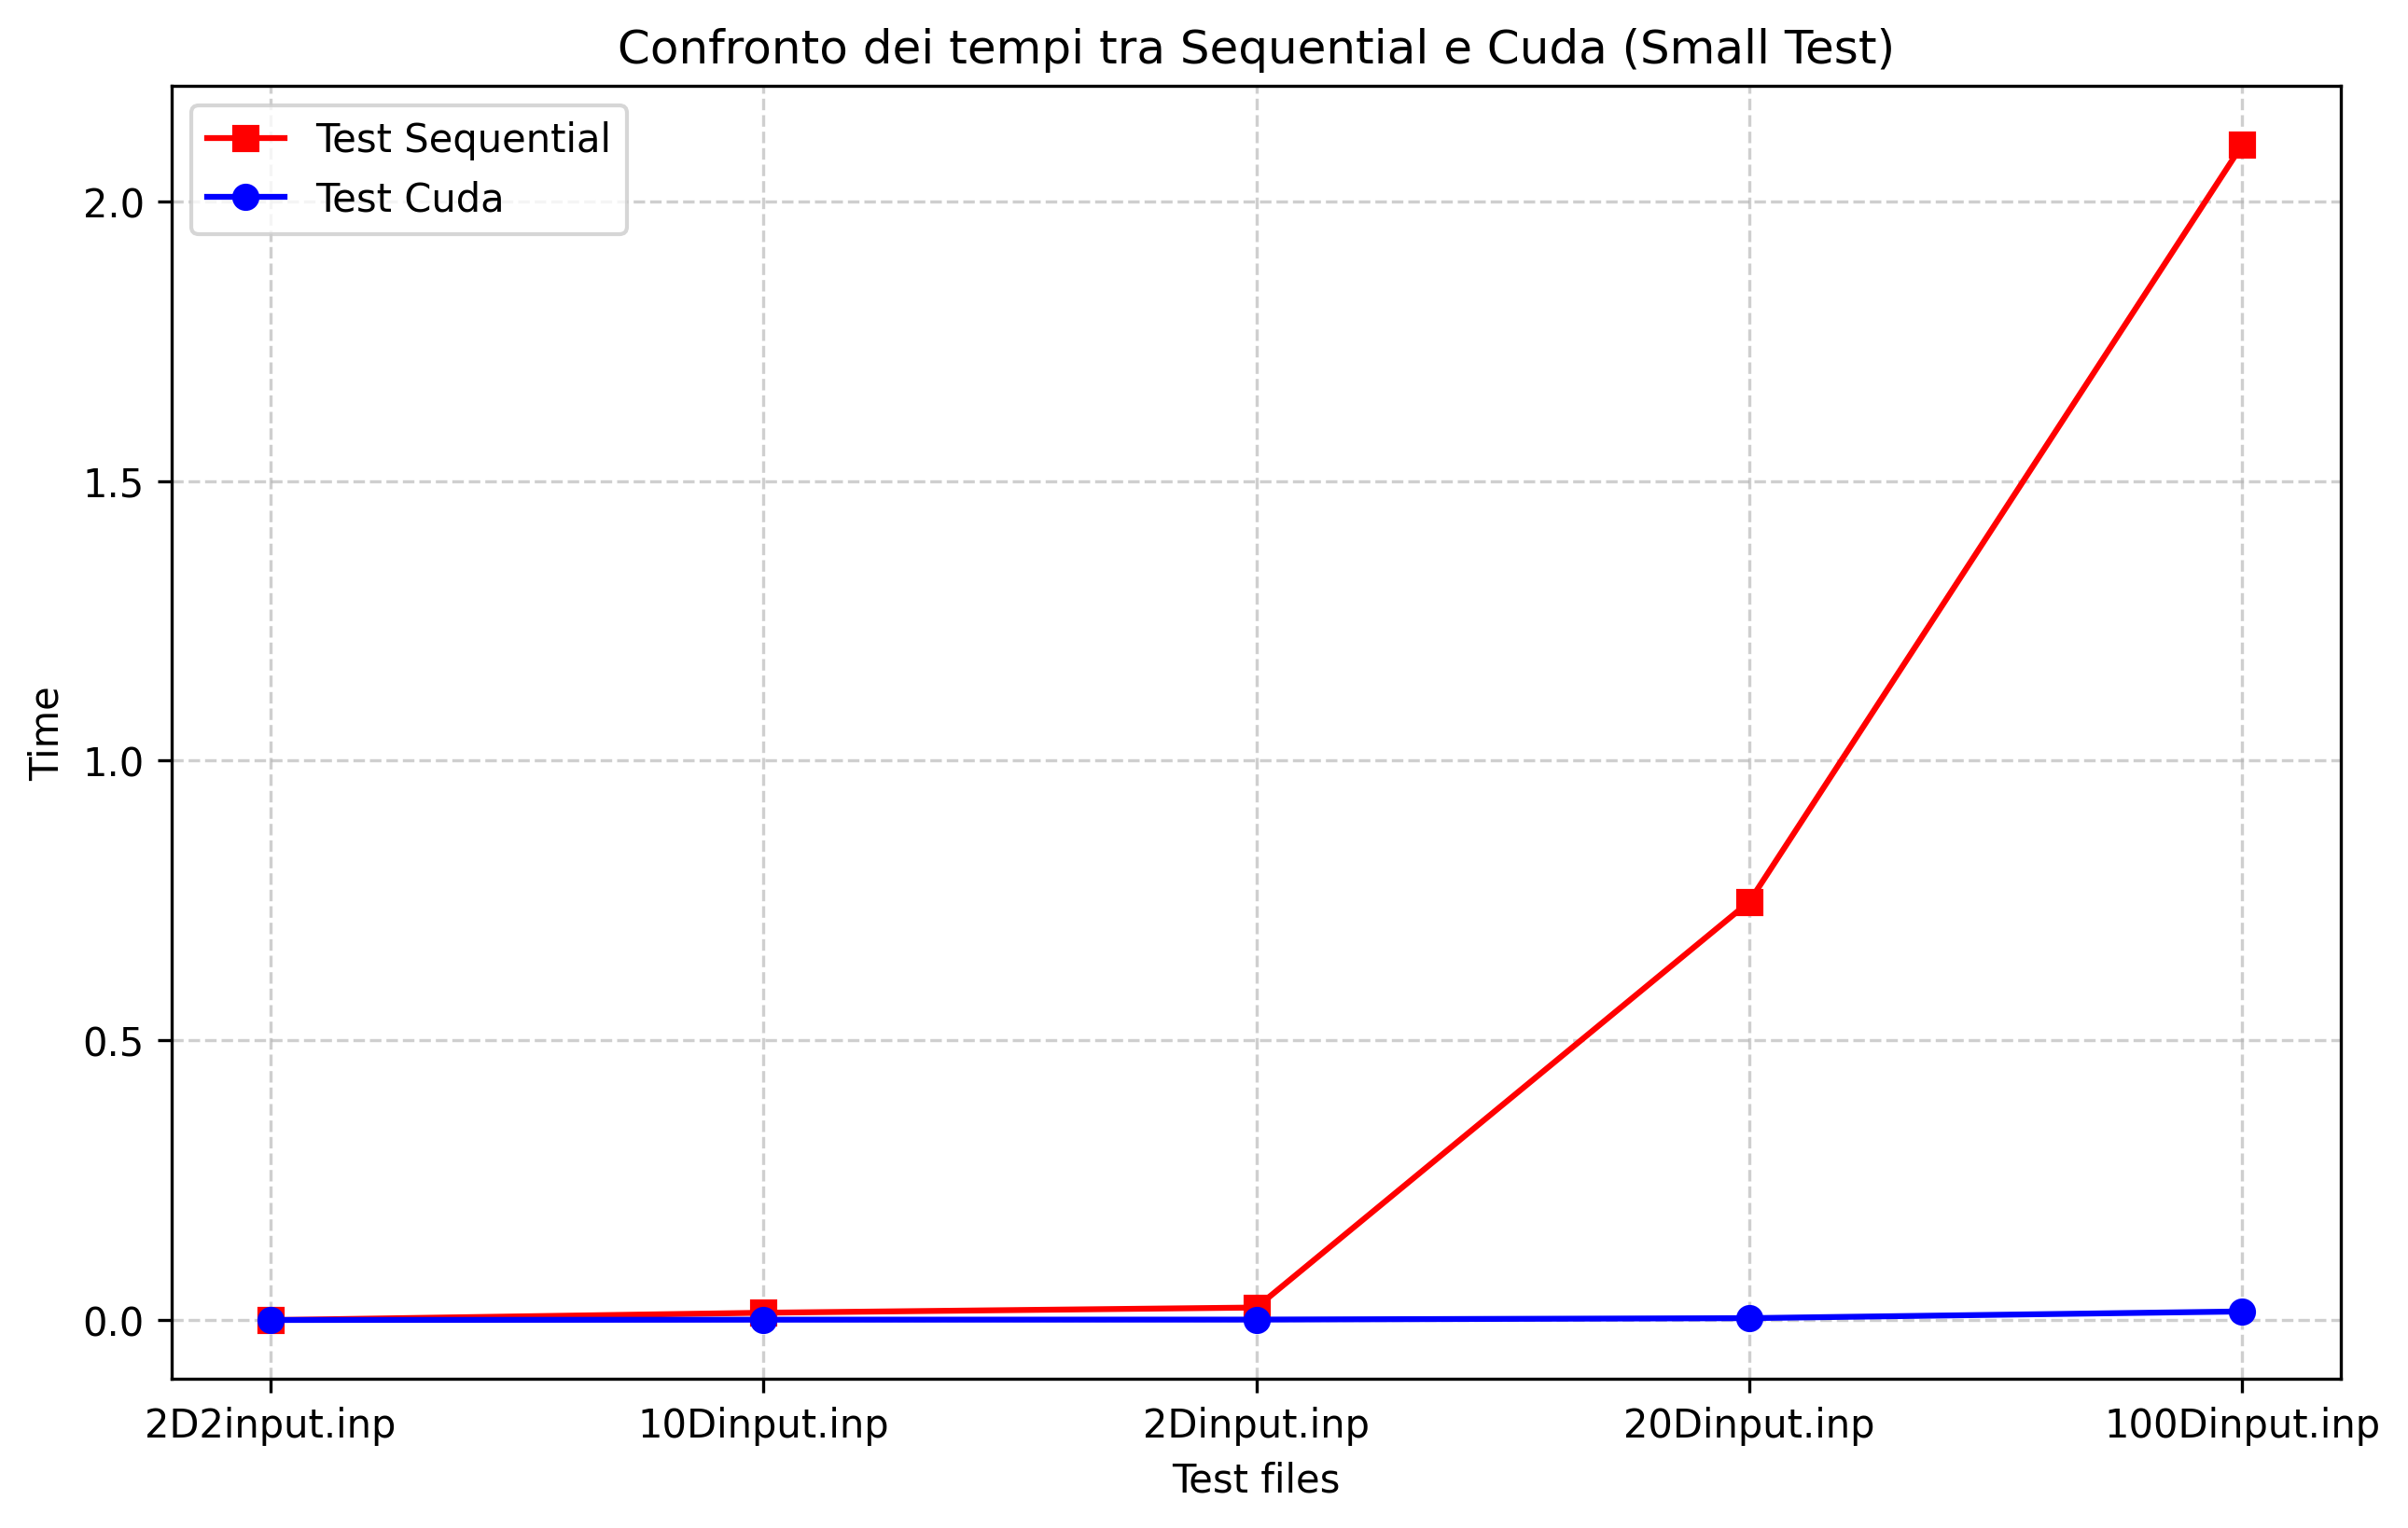
\includegraphics[width=\linewidth]{../test_csv/plots/plot_cuda_small_slurm.png}
    \end{minipage}
    \begin{minipage}{0.45\textwidth}
      \centering 
      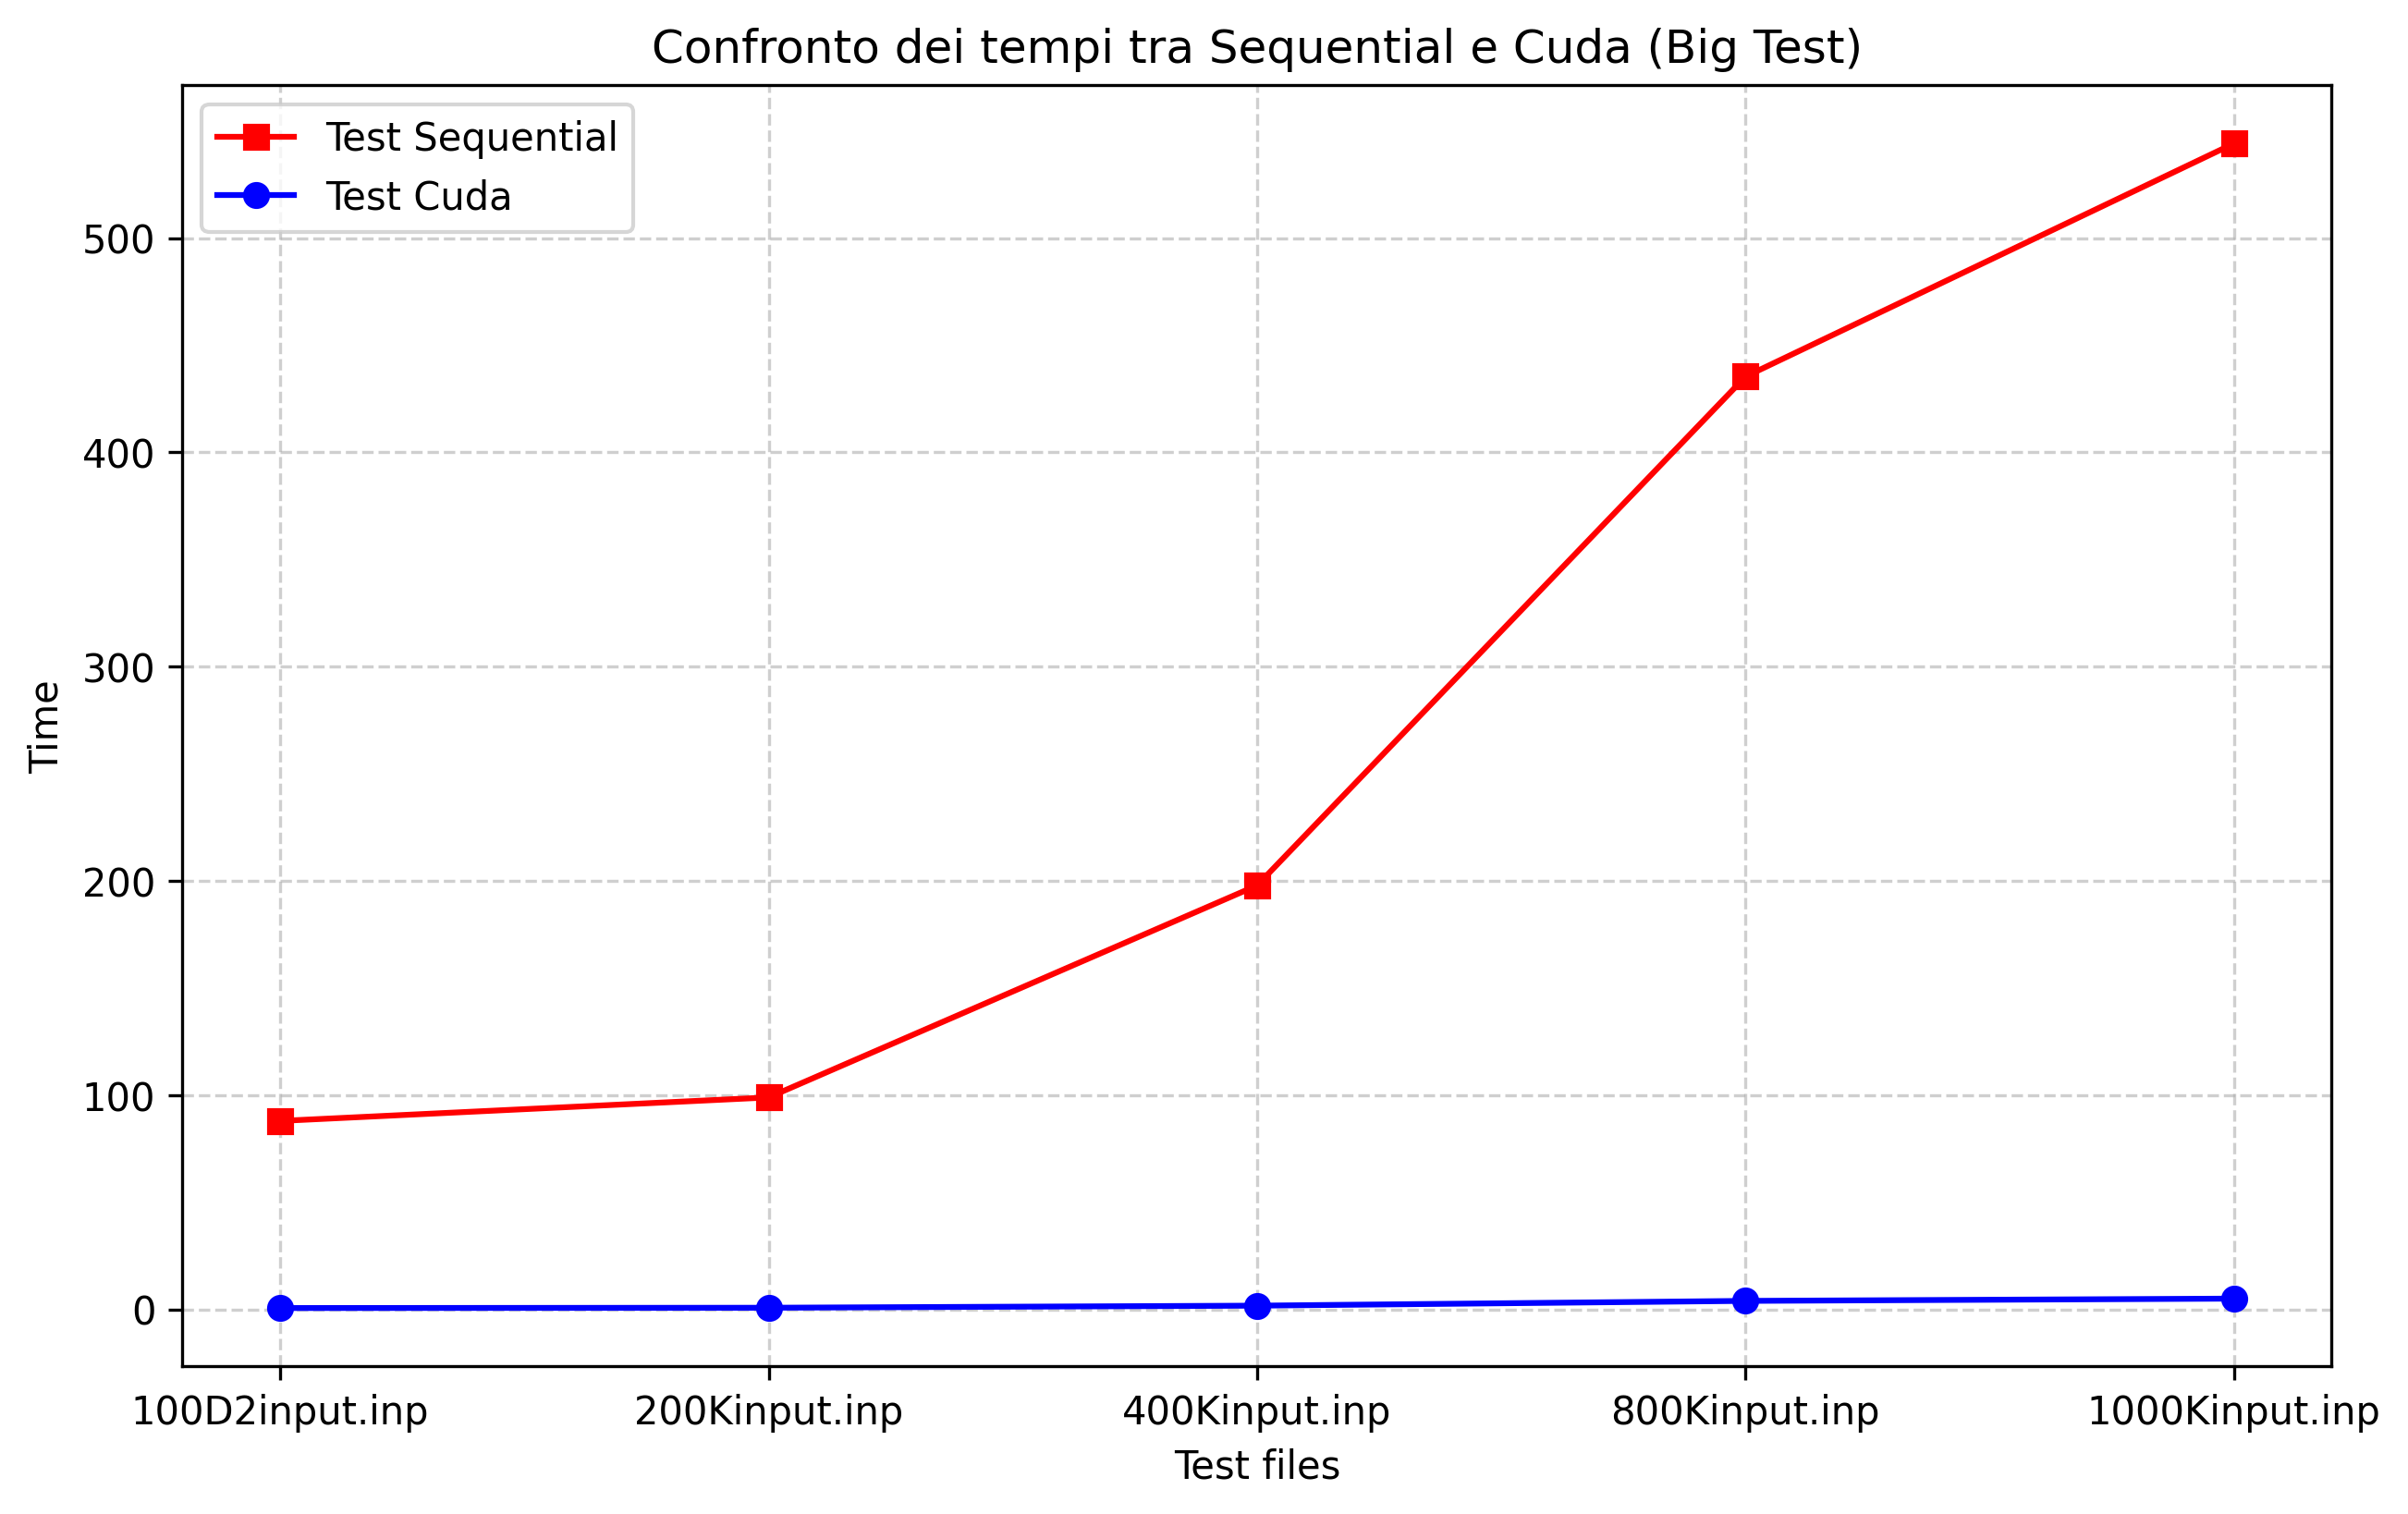
\includegraphics[width=\linewidth]{../test_csv/plots/plot_cuda_big_slurm.png}
    \end{minipage}
  \end{figure}
  \begin{center}
    \small *Nel cado di CUDA, in questi grafici sono riportati i tempi utilizzando 256 thread per blocco
  \end{center}

  Da questi grafici possiamo notare la differenza di tempo di esecuzione tra le due versione, ovviamente, nei test più leggeri la versione di cuda non è molto efficente in quanto essendo la mole di dati da elaborare molto bassa 
  la versione di CUDA perde tempo per l'allocazione della memoria e il trasferimento dei dati dalla CPU alla GPU, mentre nei test più pesanti la versione di CUDA è molto più efficente rispetto a quella sequenziale, in quanto 
  il sequenziale avendo una mole di dati molto alta, ha un costo computazionale molto più alto rispetto alla versione CUDA, che riesce a parallelizzare il lavoro tra i vari core della GPU.
  
  \begin{center}
    \rule{2.5cm}{1pt} \makebox{\texttt{Speedup}} \rule{2.5cm}{1pt}
  \end{center}
  \begin{figure}[ht]
    \centering
    \begin{minipage}{0.45\textwidth}
      \centering
      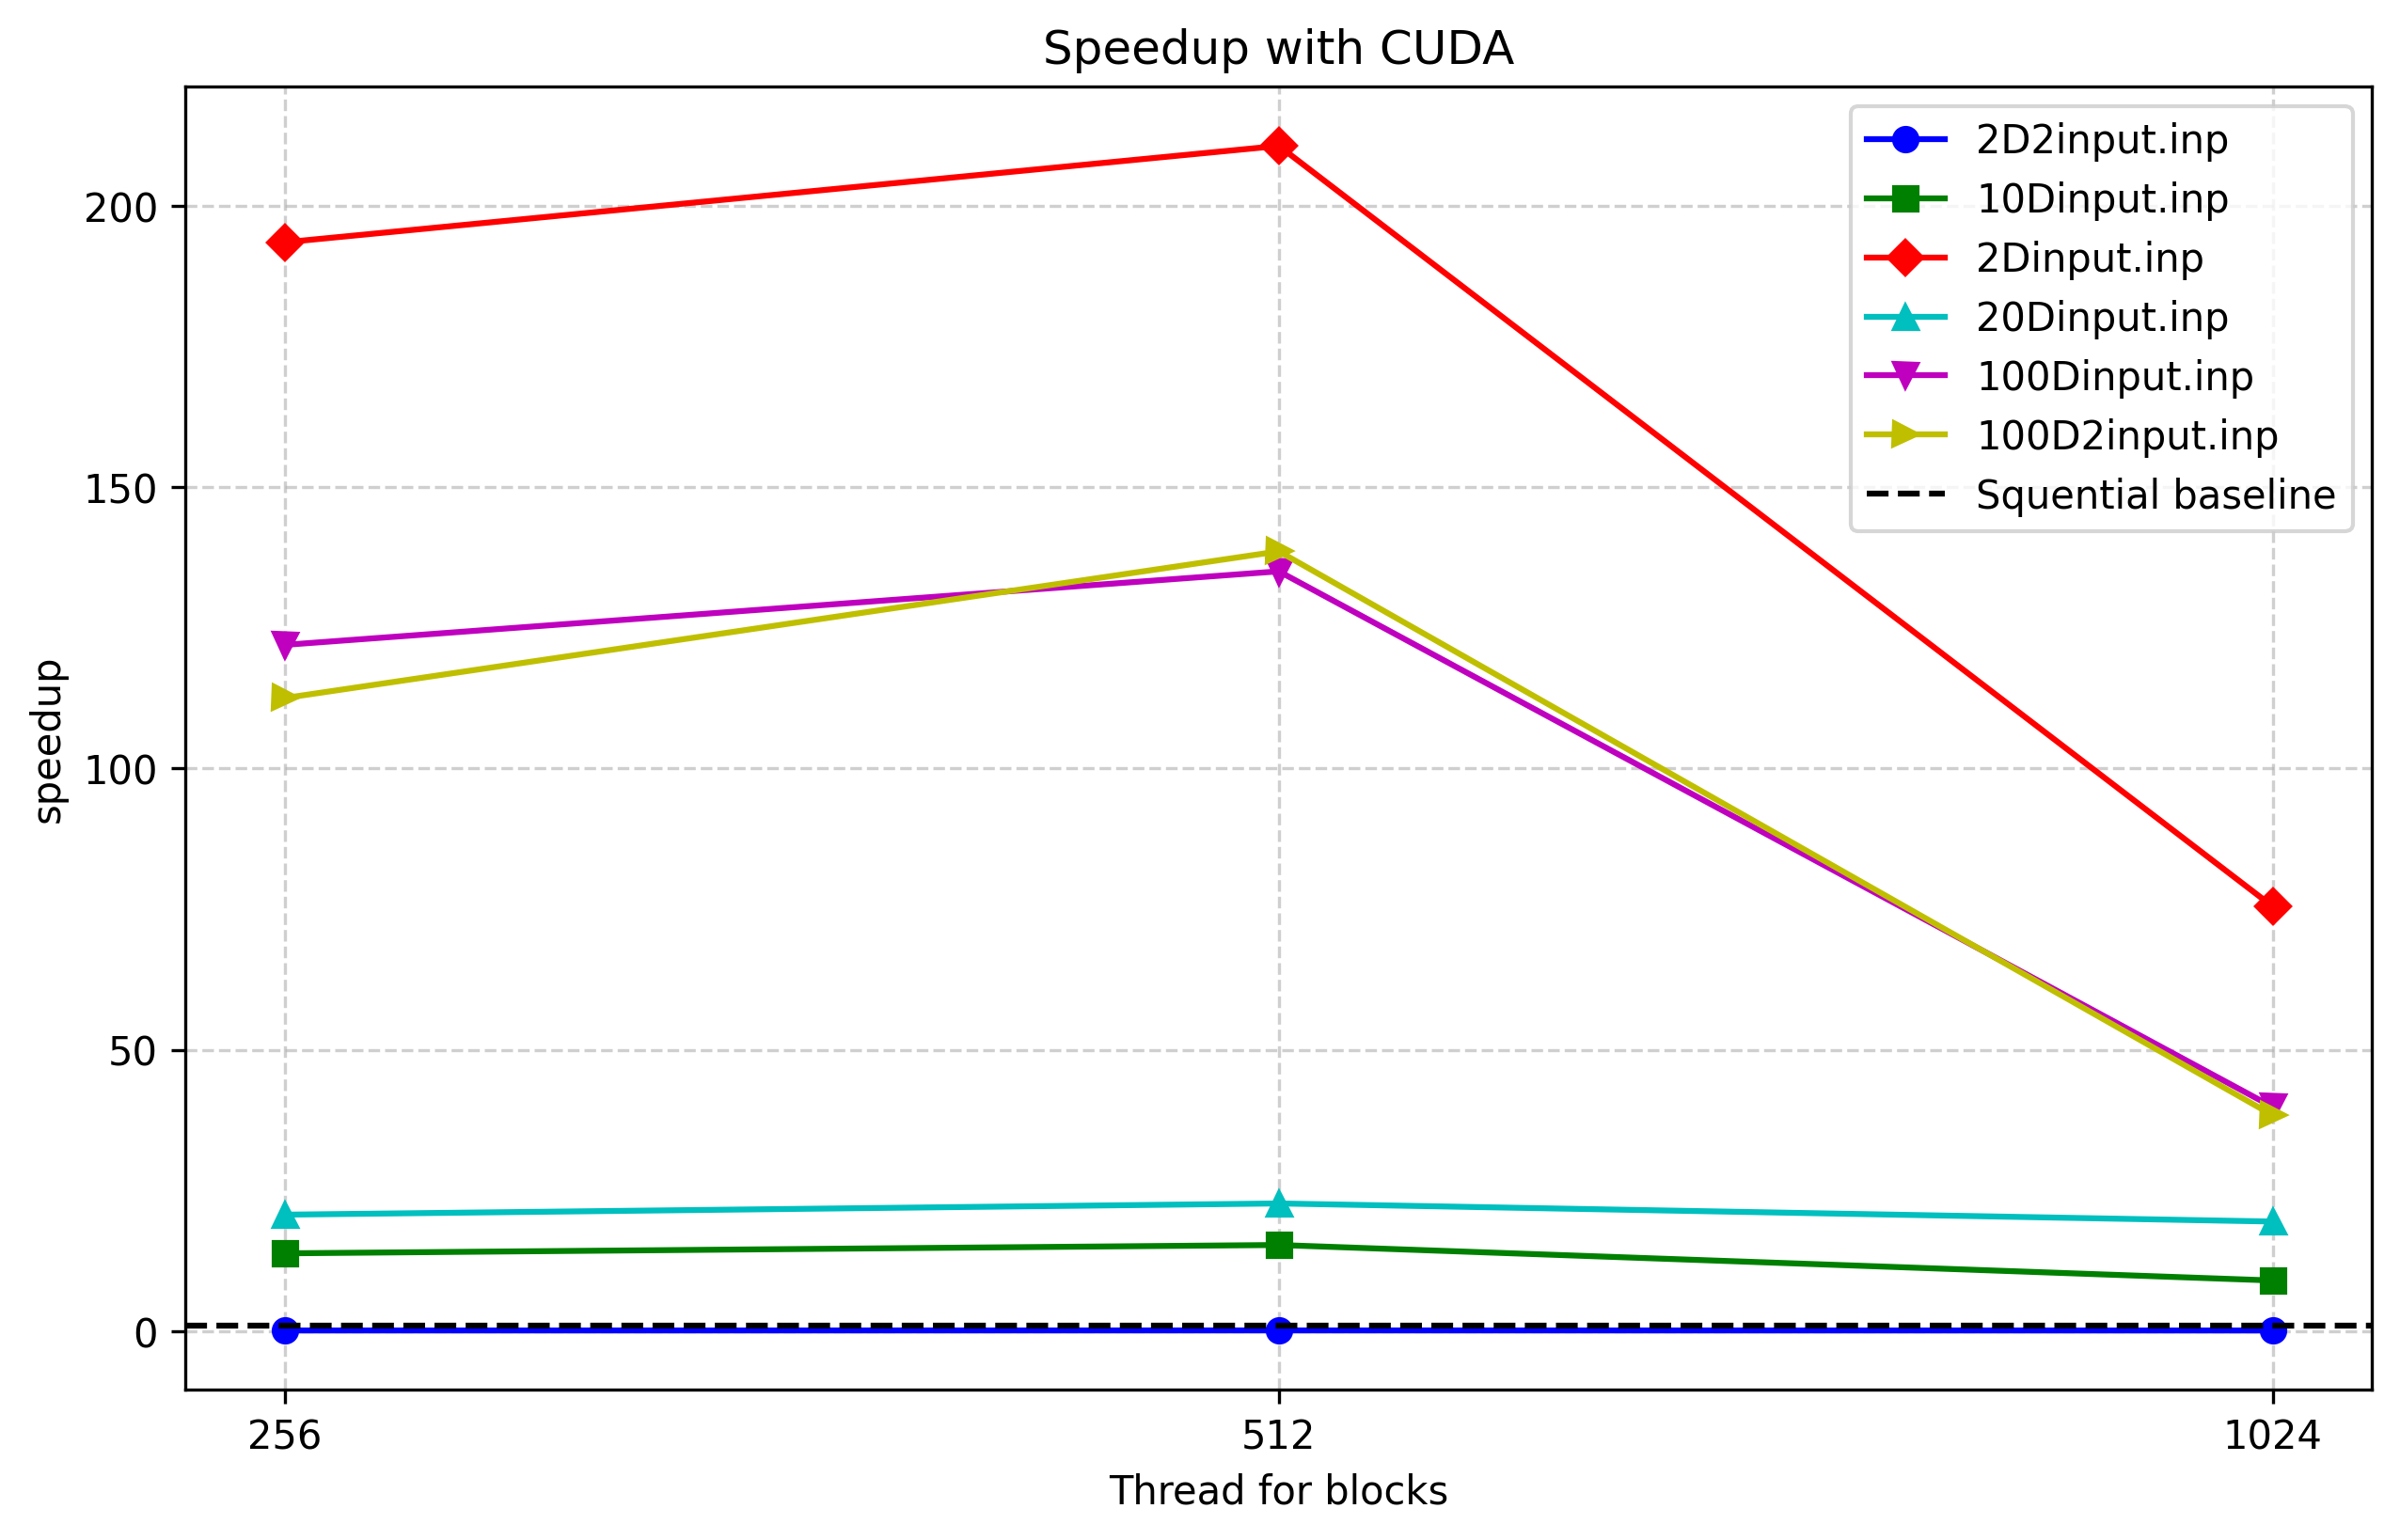
\includegraphics[width=\linewidth]{../test_csv/plots/speedup/plot_cuda_small_slurm.png}
    \end{minipage}
    \begin{minipage}{0.45\textwidth}
      \centering
      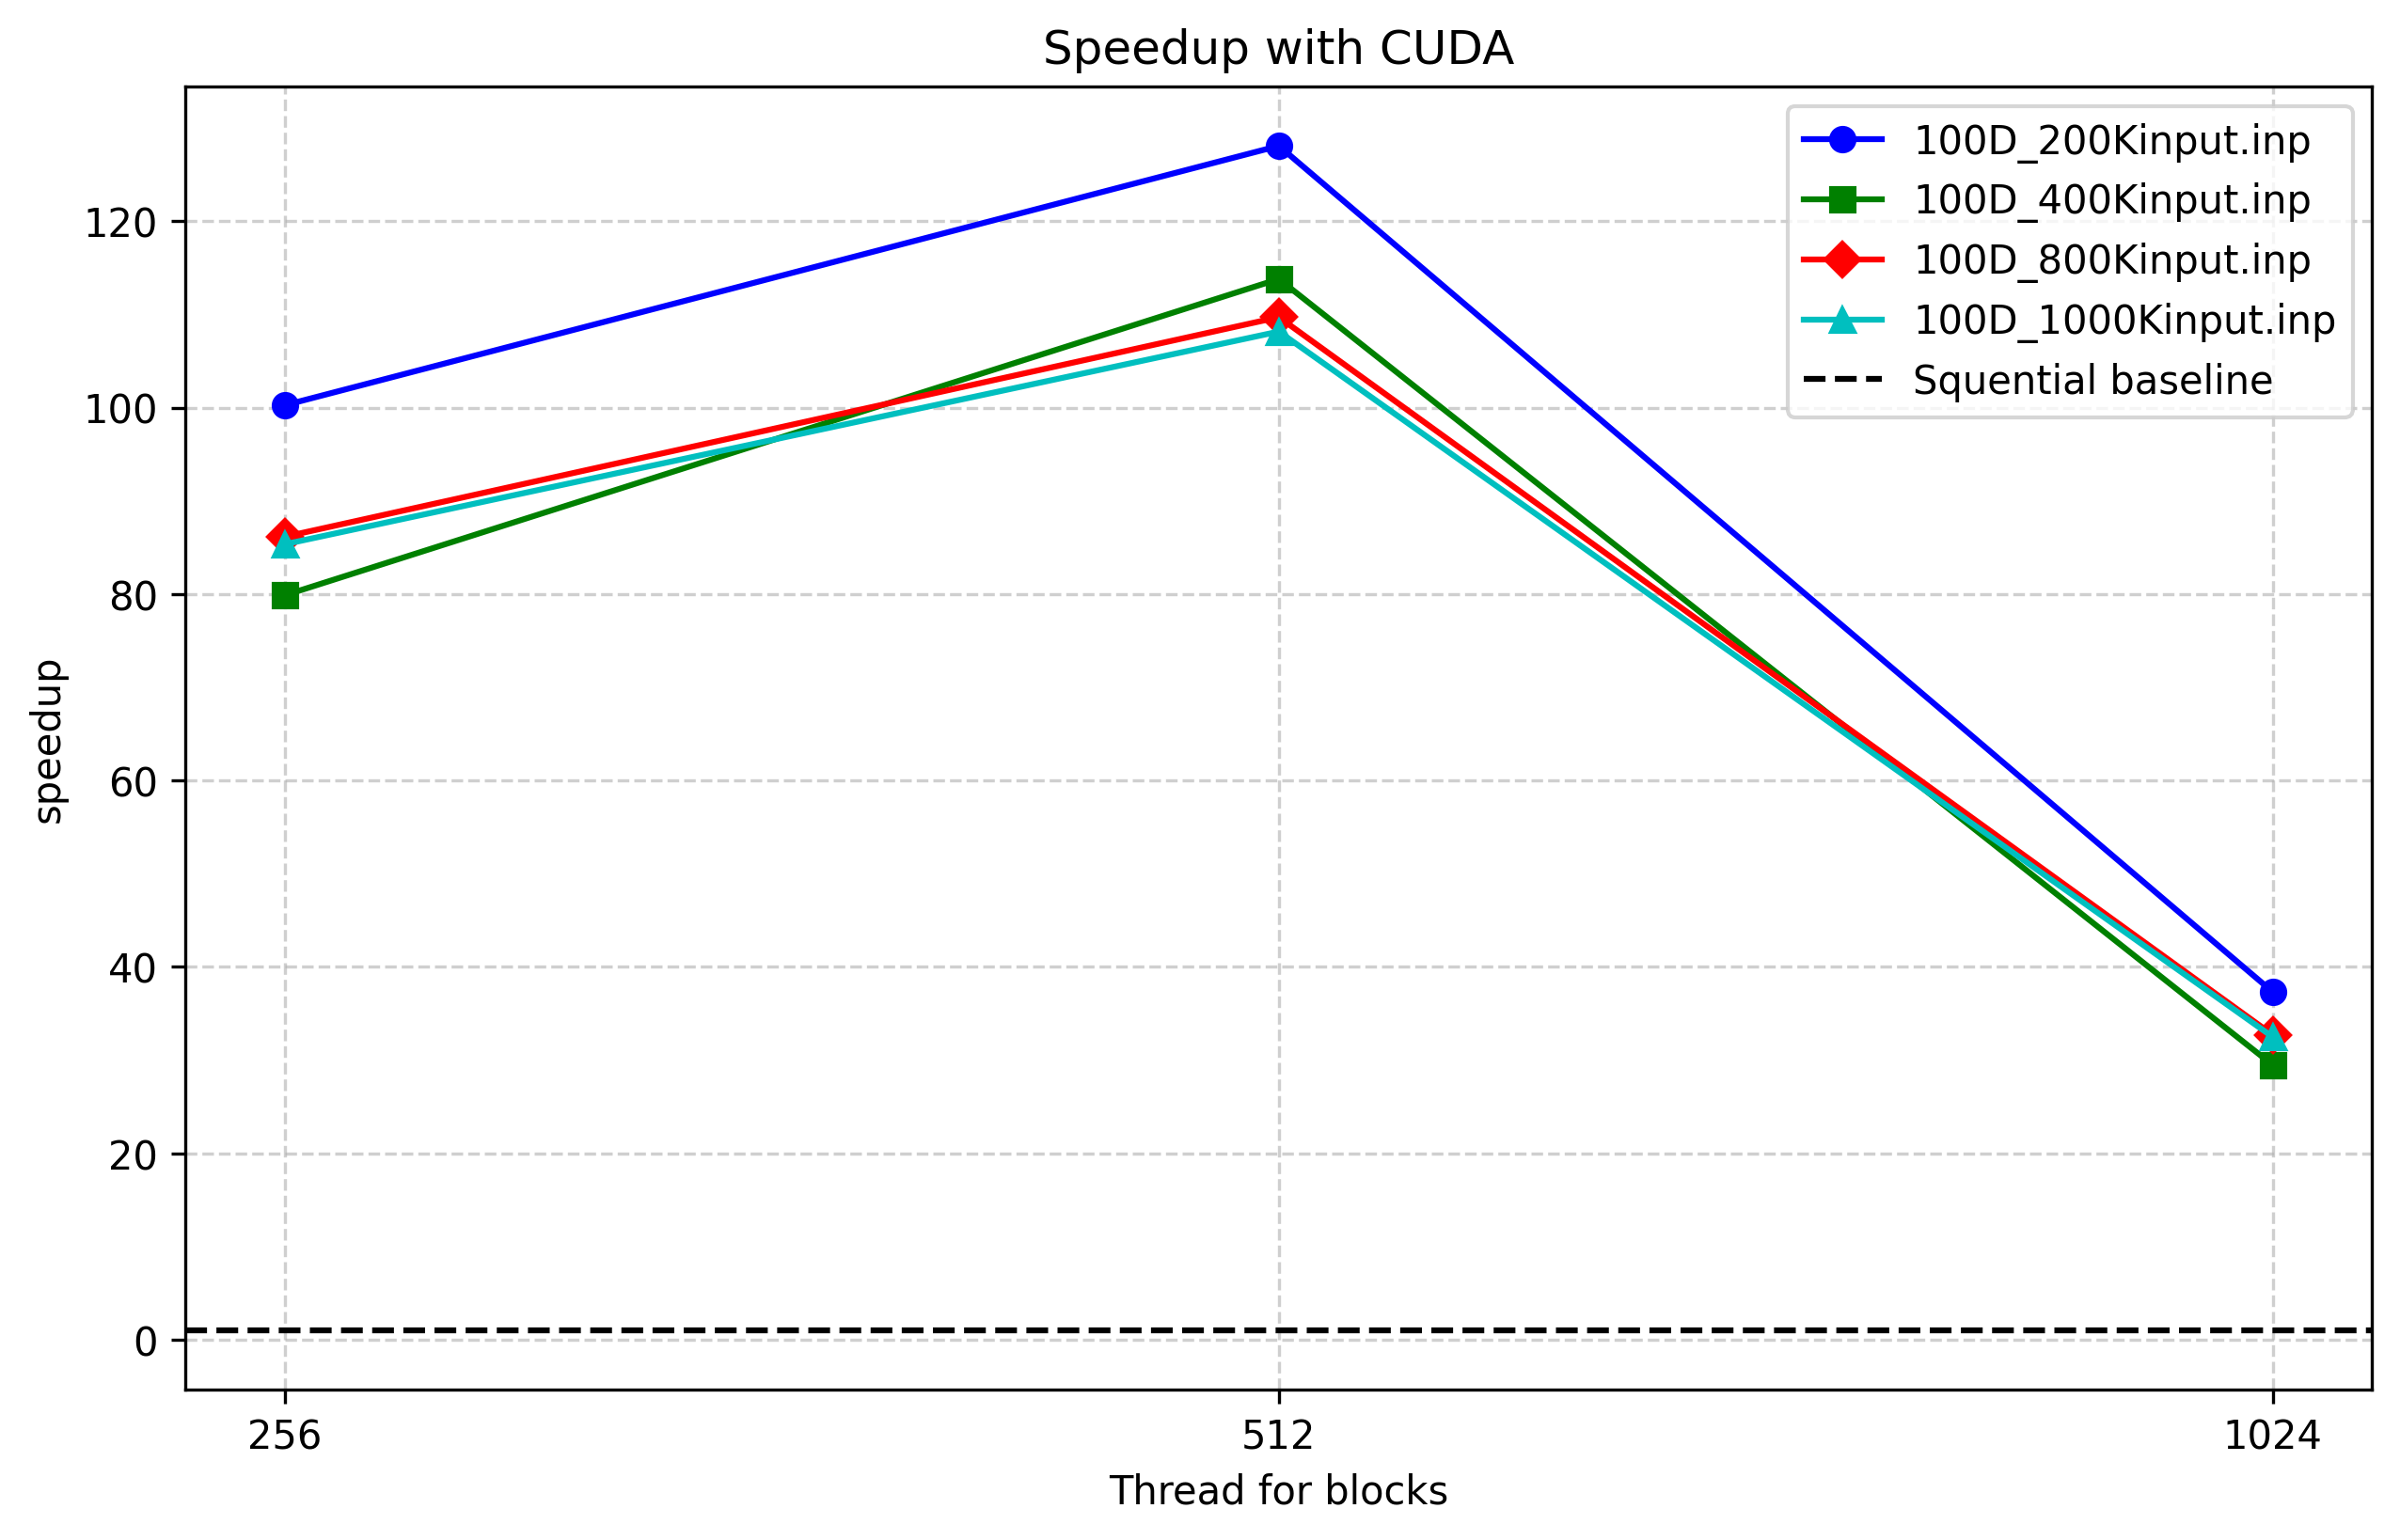
\includegraphics[width=\linewidth]{../test_csv/plots/speedup/plot_cuda_big_slurm.png}
    \end{minipage}
  \end{figure}
  Da questi test possiamo notare che la versione CUDA ha uno speedup che cresce con l'aumentare della mole di dati da elaborare, ma notiamo subito che
  i risultati migliori sono ottenuti utilizzando 512 thread per blocco. Utilizzando 1024 thread per blocco, lo speedup diminusice; dato che 
  il numero di thread massimo per SM è di 2048 nella \textbf{Quadro RTX 6000} (GPU utilizzata all'interno del cluster), utilizzando 1024 thread per blocco si hanno 32 warp per blocco, di conseguenza il numero di context switch tra warp è molto alto, causando 
  rallentamenti sul tempo di esecuzione. Mentre con 256 e 512 il numero di context switch è minore perchè i blocchi hanno meno warp per blocco ma più blocchi per SM. Se si considera 
  il numero di context switch logicamente i thread per blocco ideale sono 256, tuttavia, il numero di thread per blocco più efficente è 512 come possiamo notare dal grafico,
  questo causato dal fatto che essendo un kernel molto pesante, il numero di context switch non ha un impatto significativo sul tempo di esecuzione, se si utilizzano 256 thread 
  i warp che vengono eseguiti in parallelo sono minori rispetto a quelli che vengono usati con 512 thread.

  \begin{center}
    \rule{2.5cm}{1pt} \makebox{\texttt{Roofline Model}} \rule{2.5cm}{1pt}
  \end{center}
 
  \begin{figure}[ht]
    \hspace*{-1.1cm}  % regola il valore a piacere
    \centering
    \begin{minipage}{0.50\textwidth}
      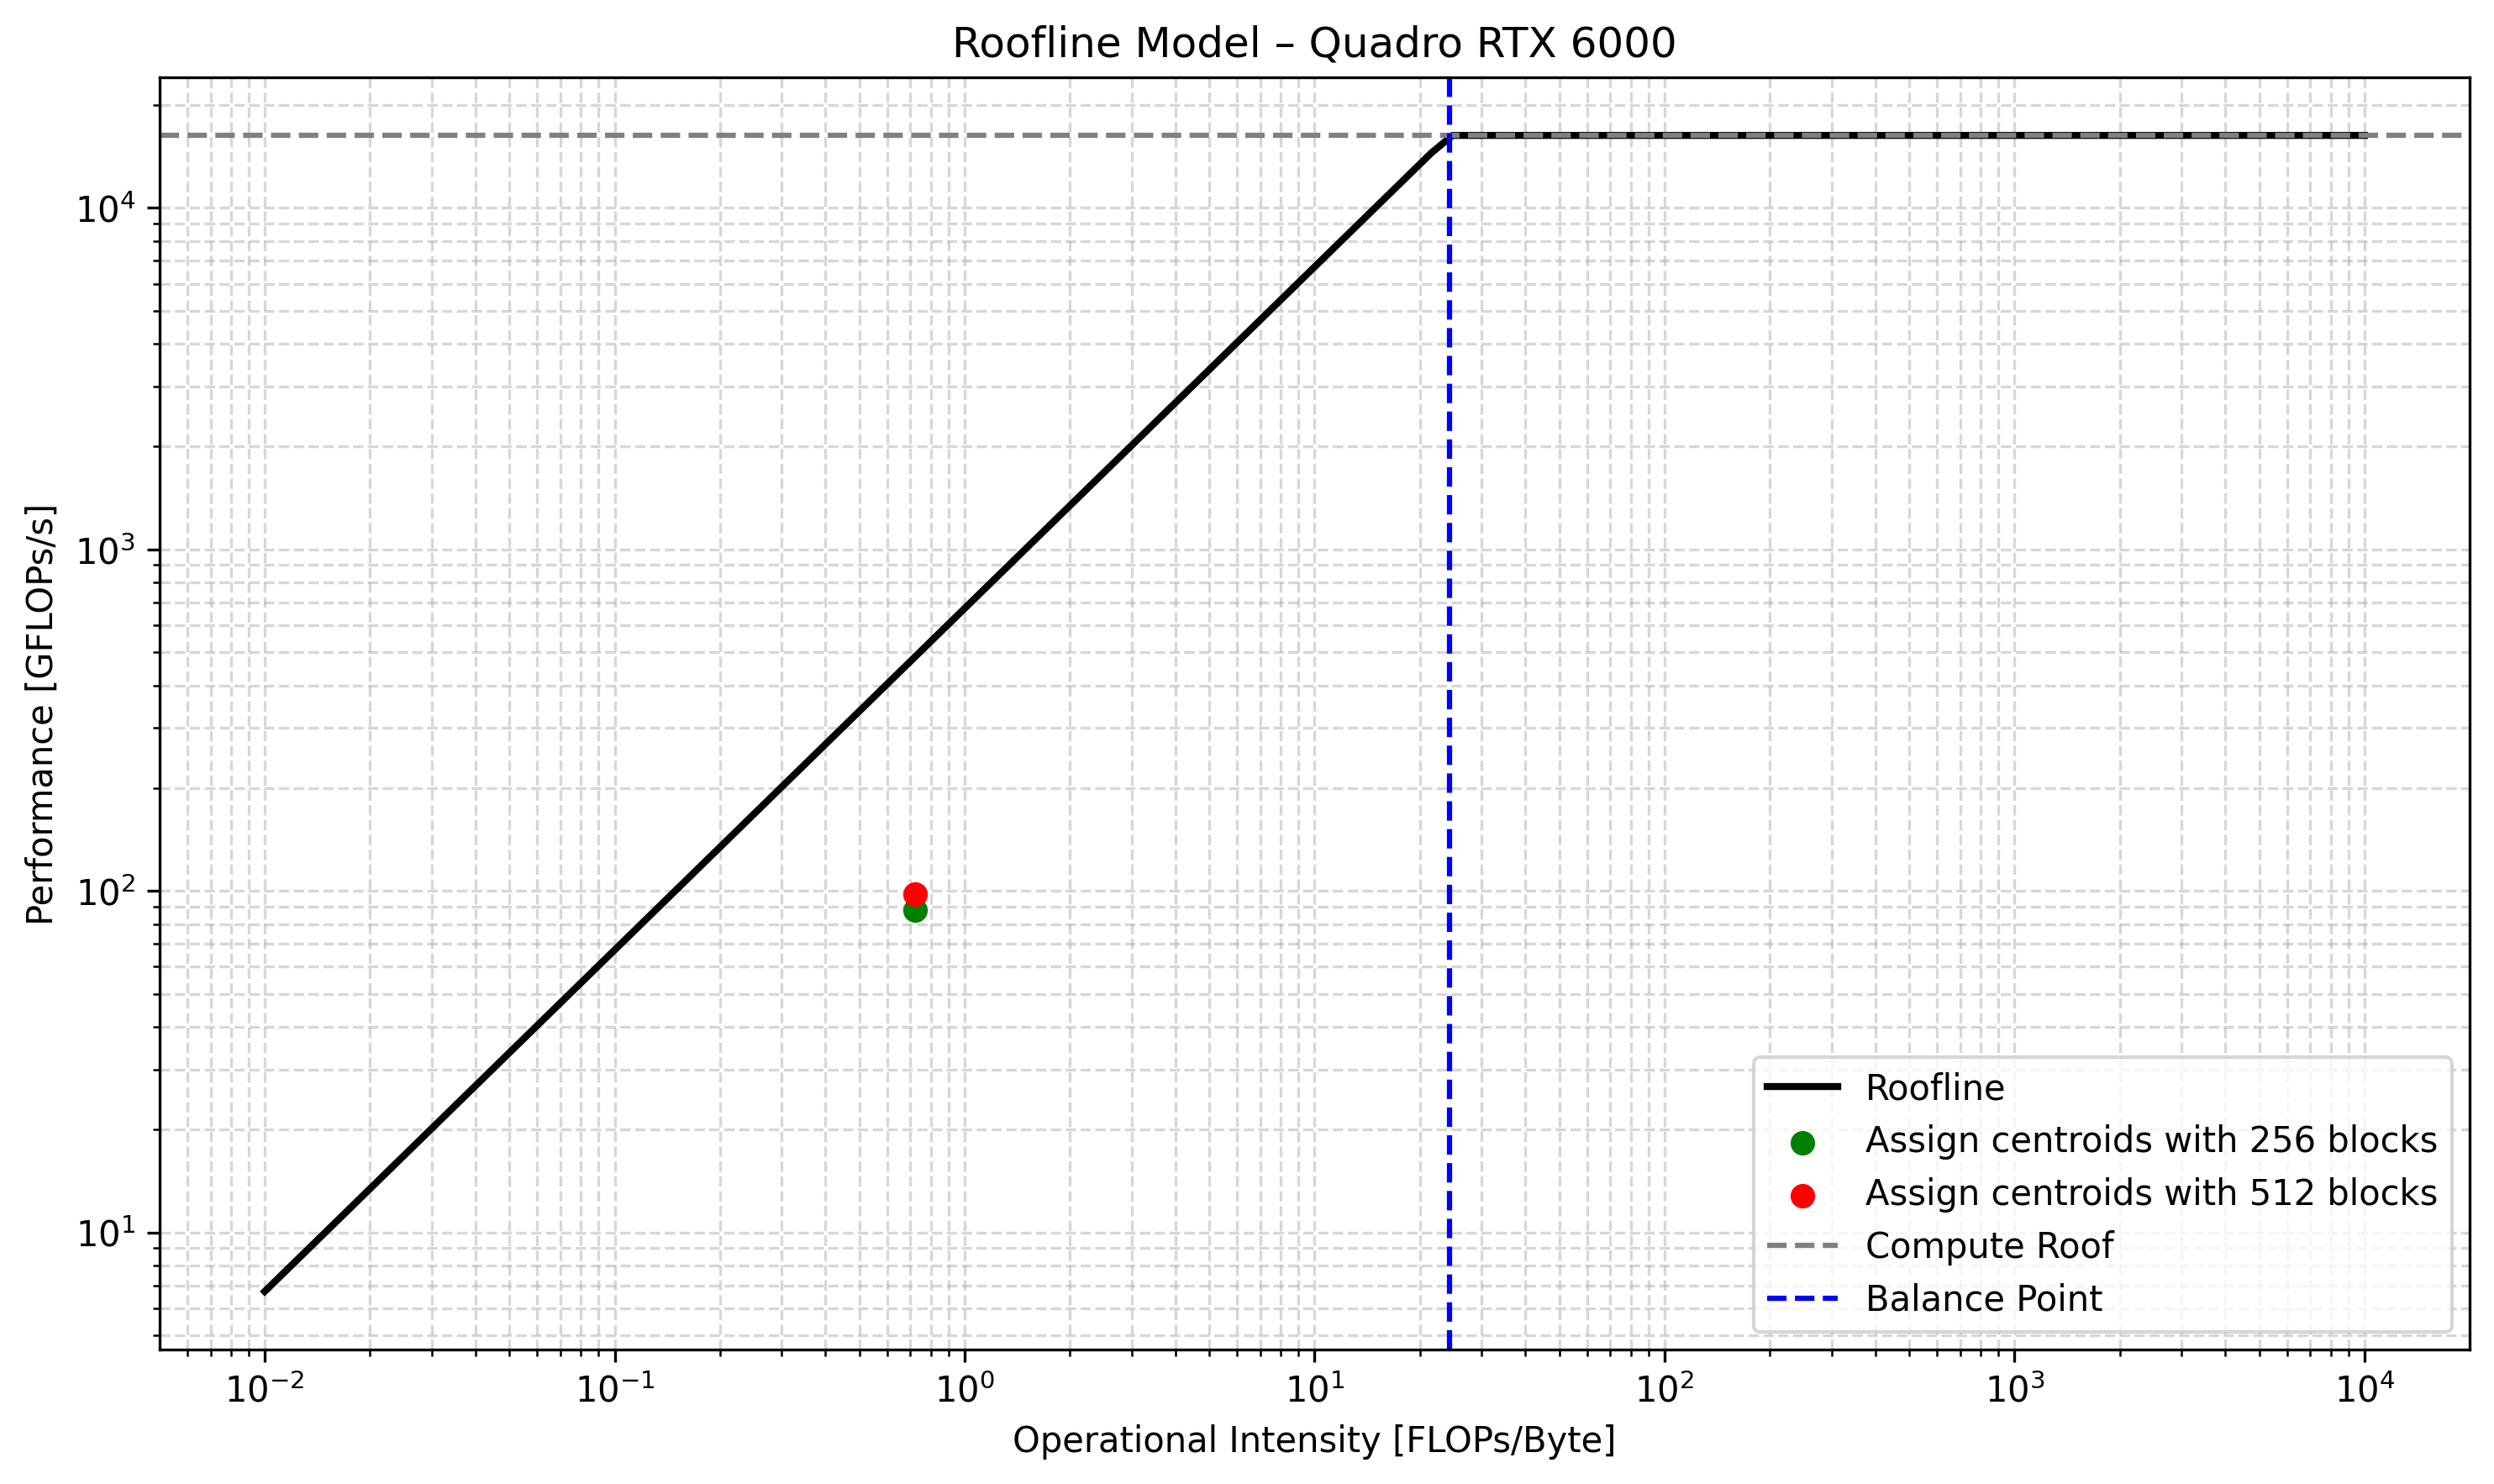
\includegraphics[width=\linewidth]{../test_csv/plots/roofline_cuda.png}
    \end{minipage}
  \end{figure}

  Possiamo notare anche nella roofline model che con 512 thread per blocco sul primo kernel si ha una performace migliore rispetto ai 256 thread, in quanto vengono eseguiti un numero maggiore di 
  GFLOP/s. Un importante dettaglio che possiamo notare da questo grafico è quanto la \textbf{global memory} influisce sul nostro programma, difatti, possiamo notare 
  che il primo kernel del programma soffre di \textbf{memory bound}, ovvero, il continuo accesso alla VRAM rallenta l'esecuzione della funzione. Per aumentare 
  le performance del kernel, si potrebbe utilizzare la \textbf{shared memory} per salvare i dati che vengono utilizzati più volte, diminuendo così la 
  \textbf{bandwidth}, ma cercando di non occupare molto la shared memory, in quanto è una memoria \textbf{cache L1} condivisa da i core della GPU e non ha una grande capienza.

  \begin{center}
    \rule{2.5cm}{1pt} \makebox{\texttt{Time distribution, median and avarage}} \rule{2.5cm}{1pt}
  \end{center}
  \begin{figure}[ht]
    \centering
    \begin{minipage}{0.45\textwidth}
      \centering
      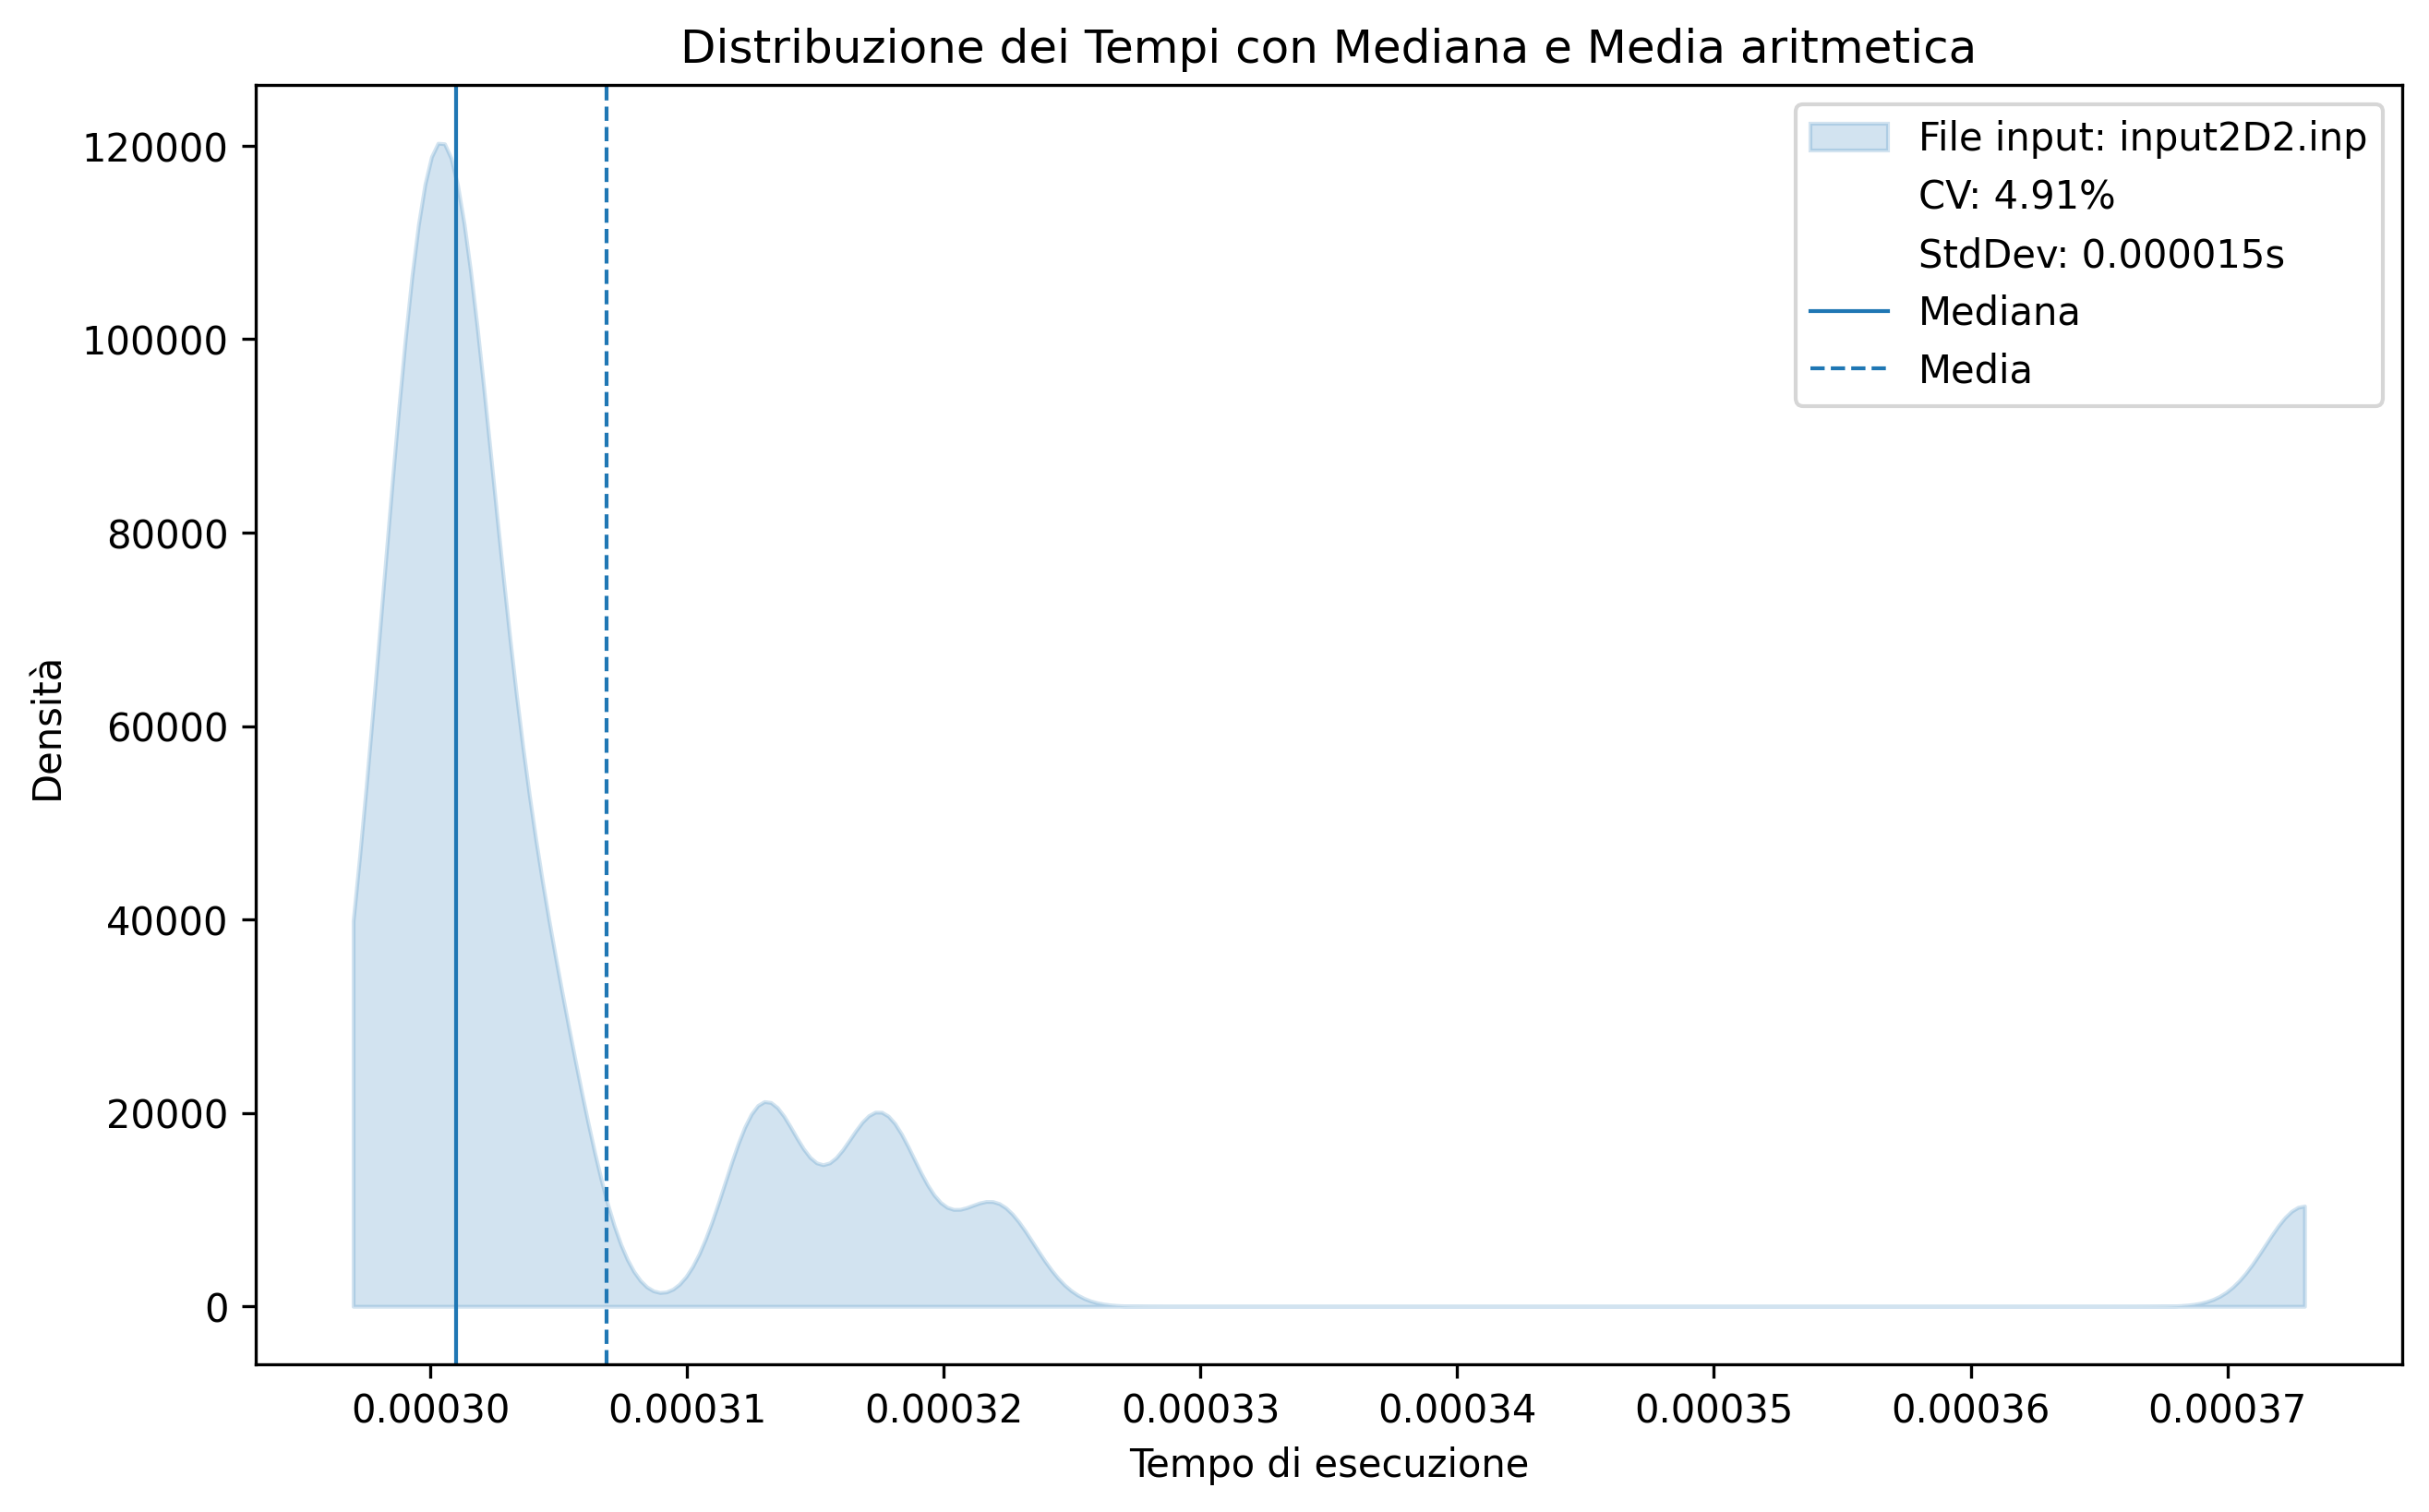
\includegraphics[width=\linewidth]{../test_csv/plots/time_distribution/time_distribution_2D2_cuda.png}
    \end{minipage}
    \begin{minipage}{0.45\textwidth}
      \centering
      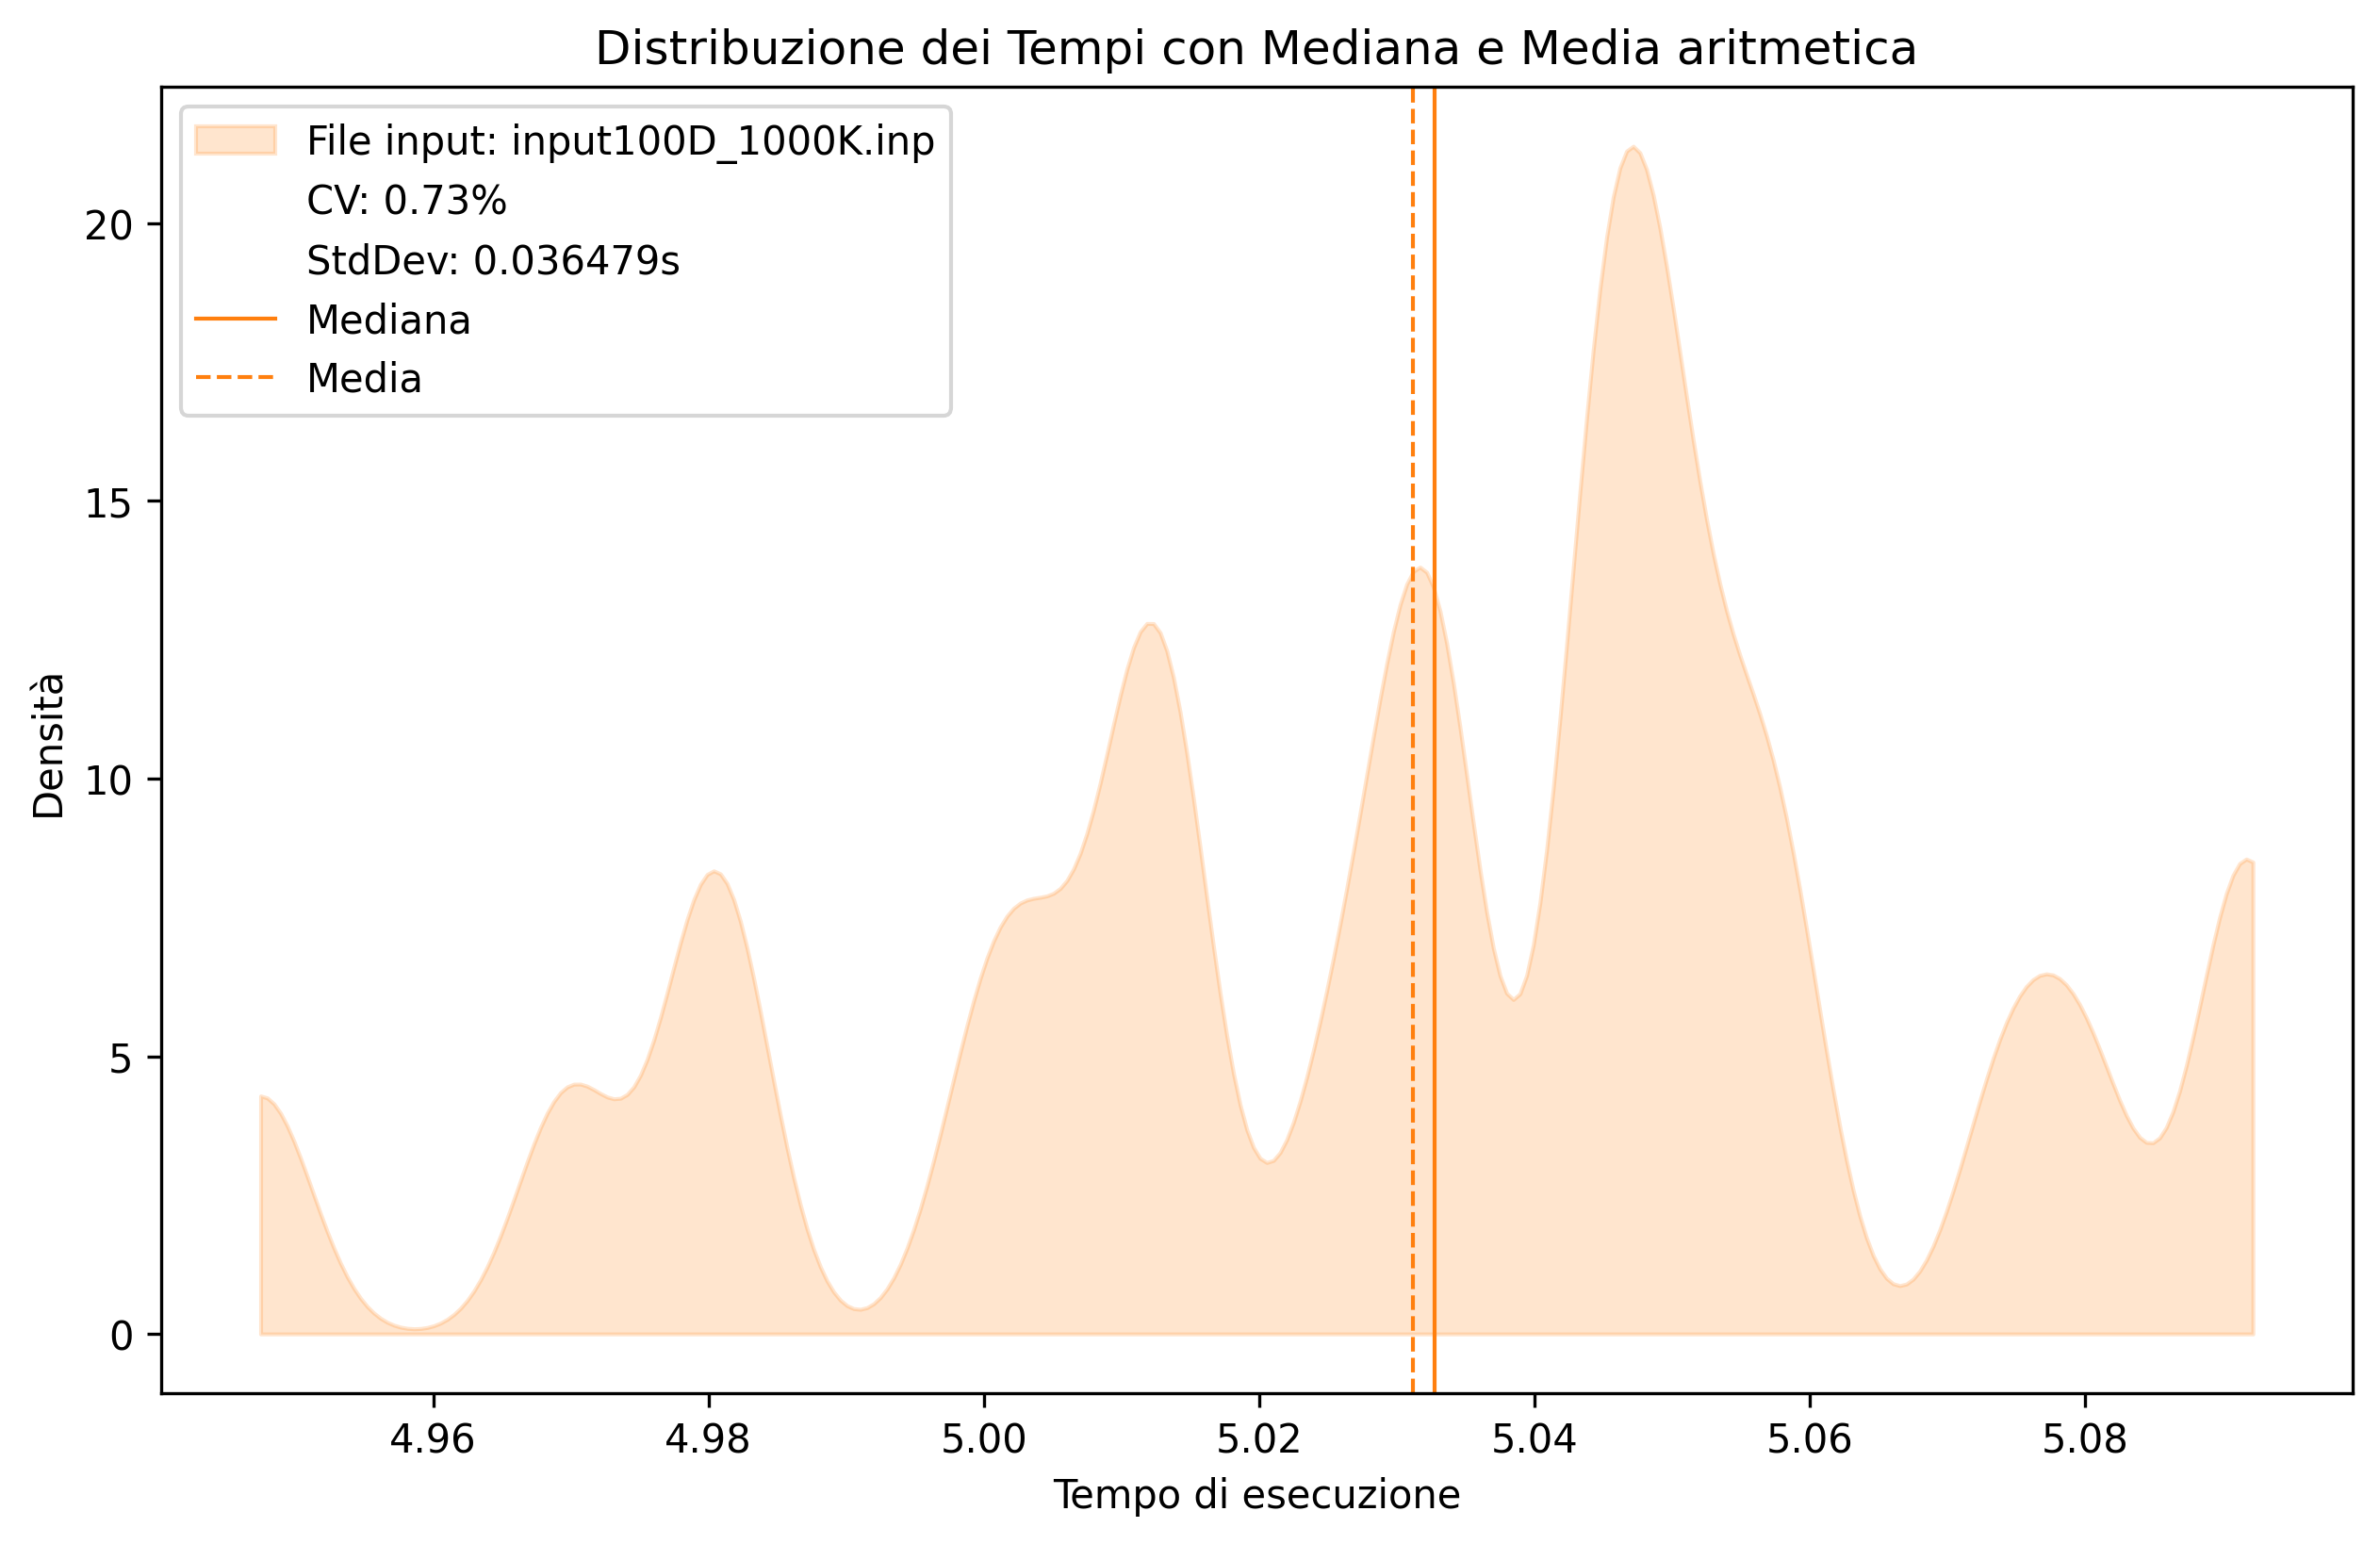
\includegraphics[width=\linewidth]{../test_csv/plots/time_distribution/time_distribution_100D_1000K_cuda.png}
    \end{minipage}
  \end{figure}

  I due grafici riportati rappresentano la distribuzione dei tempi su due file test, quello più leggero e quello più pesante, impostando il numero di thread per blocchi a 
  512. Possiamo notare che la distribuzione con il test \verb|1000K| ha dei buoni valori, in quando sia la mediana che la media sono molto vicini tra loro, questo indica che 
  i tempi sono molto stabili. Lo possiamo notare anche dal \textbf{coefficente di variazione} in quanto vale \verb|0.73%| indicando che i tempi dei vari test non hanno subito 
  troppi oscillazzioni, infine, anche se non viene rappresentato un grafico a campana, i tempi sembrano essere ben distribuiti. 
  Per quanto riguarda il test \verb|2D2| possiamo notare subito delle differenza, la mediana e la media non sono molto vicini tra loro questo segna poca stabilià tra i tempi, anche 
  il \textbf{coefficente di variazione} ha un valore significativo; un'altra importante differenza lo si nota sulla coda che si viene a creare verso destra con un leggero picco 
  finale, questo dimostra che tra i vari test ci sono stati alcuni test più lunghi di altri. Tuttavia, stiamo analizzando dei tempi molto piccoli lo si nota dalla deviazione standard, 
  di conseguenza, alcuni test sono più lunghi di altri perchè hanno impegato legggermente più tempo nella copia dei dati tra CPU e GPU o viceversa.

  \section{MPI and OMP Version}

  La prima modifica effettuata per la realizzazione di questa versione è partita con l'inizializzazione del dei processi \textbf{MPI}, infatti, per utilizzare \textbf{OpenMP} insieme a \textbf{OpenMPI} l'inizializzazione viene effettuata con 
  \verb|MPI_Init_thread(&argc, &argv, MPI_THREAD_FUNNELED, &provided)| in modo tale da  garantire la gestione dei thread in modo da non avere problemi di concorrenza, in particolare viene utilizzato \verb|MPI_THREAD_FUNNELED| in modo che ogni processi 
  abbia il modo di creare il numero di thread che gli viene specificato.
  Un'altra modifica effettuata all'interno del codice è stata eseguita per quanto riguardano i parametri presi in input, in quanto viene specificato il numero di thread da utilizzare come ultimo argomento:
  \begin{center}
    \verb|./KMEANS_omp_mpi ... [Number of OMP threads]|
  \end{center}

  Prima della sezione \verb|do - while| venogno divisi in modo equo per ogni processo l'inizio e la fine della porzione degli array su cui devono eseguire i vari calcoli e viengono impostati i thread da utilizzare con la funzione 
  \verb|omp_set_num_threads()|. In particolare, vengono creati due array: \verb|recvcounts|; \verb|displs|; utilizzati come buffer di appoggio per l'utlizzo della funzione \verb|MPI_Allgatherv|, utilizzata per condividere l'array classMap tra tutti i processi invnece di 
  \verb|MPI_Allgather|, in seguito vengono divisi in modo equo gli elementi su cui devono lavorare i processi, ecco un esempio sulle linee:
  \begin{lstlisting}[language=C]
  int local_lines = lines / size;
  int start_line = rank * local_lines;
  int end_line = (rank == size - 1) ? lines: start_line + local_lines;
  \end{lstlisting}
  \subsection{Parallelization with OpenMP}
  Dopo i vari calcoli e la divisione tra i processi all'interno del ciclo \verb|do - while| vengono utilizzati vari funzioni di \textbf{MPI} per la comunicazione tra i vari processi e vengono utilizzati i pragma \textbf{OpenMP} per la parallelizzazione dei 
  vari for all'interno del ciclo. Per quando riguarda la seconda sezione [\ref{s_section}] citata nell'introduzione, viene utilizzato il seguente pragma:
  \begin{lstlisting}[language=C]
    # pragma omp parallel for private(j,class,dist,minDist) \
        reduction(+:local_changes) \
        reduction(+:pointsPerClass[:K],auxCentroids[:K*samples])
  \end{lstlisting}
  Viene utilizzato: 
  \begin{enumerate}
    \item \verb|private()| per dichiarare le variabili che rimangono private per ognid thread, e che non vengono condivise tra i vari thread in modo per non avere problemi di concorrenza; 
    \item \verb|reduction(+:local_changes)| per gestire i problemi di concorrenza quando più thread aggiornano la variabile; \verb|local_changes|; 
    \item \verb|reduction(+:pointsPerClass[:K],auxCentroids[:K*samples])| in modo tale che non si riscontrano problemi di concorrenza quando viene eseguita l'operazione di somma su un elemento dei due array indicati, ovvero \verb|pointsPerClass| e \verb|auxCentroids|.
  \end{enumerate}
  Per quanto riguarda la sezione [\ref{t_section}] viene utilizzato il seguente pragma:
  \begin{lstlisting}[language=C]
    # pragma omp parallel for private(j) reduction(max:maxDist)
  \end{lstlisting}
  Invece in questo pragma viene riutilizzato il pragma \verb|private()| e in aggiunta una reduction sull'operazione \verb|max| per evitare che quanto si controlla il massimo di tale variabile, si evitano problemi di concorrenza che potrebbero 
  sovrascrivere il valore massimo con un valore sbagliato.

  \subsection{Parallelization with OpenMPI}
  Per quanto riguardano le funzioni di \textbf{OpenMPI} vengono utilizzate tra le varie sezioni citate, principalmente vengono usate le funzioni \verb|MPI_Allreduce| per eseguire operazioni di somma o max tra vari processi, infine, vengono usate le funzioni \verb|MPI_Allgatherv| e \verb|MPI_Allgather| per 
  inviare a tutti i processi gli array utilizzati.

  \begin{figure}[ht]
    \centering
    \begin{minipage}{\textwidth}
      \centering
      \includegraphics[width=\linewidth]{MPI_Func.png}
    \end{minipage}
  \end{figure}
  Molto importante l'utilizzo della funzione \verb|MPI_Allgatherv| per condividere l'array \verb|classMap| che è un array i cui 
  elementi (in base al numero di processi e il numero di linee del file di input) potrebbe non essere divisi in modo equo tra i processi, di conseguenza, tale funzione a differenza di \verb|MPI_Allgather| riesce a prendere da tutti i processi 
  il numero di elementi definito nei buffer di appoggio e unirli nell'array \verb|classMap|, senza avere l'obbligo di dover condividere in modo equo gli elementi tra i vari processi. Questa operazione viene eseguita 
  in quanto l'array classMap viene ssalvato sul file di output, di conseguenza, per non modificare la funzione writeResult, viene utilizzata questa funzione per unire i vari array classMap in uno solo, in modo tale che la funzione 
  essendo chiamata tra tutti i processi i dati sono uguali su tutti i processi.

  \subsection{Testing, speedup and efficiency}

  Per quanto riguarda la fase di testing, il programma è stato testato con vari processi e vari thread, in particolare i test sono stati eseguiti con \verb|2|, \verb|4| e \verb|8| processi, ogni processo è stato eseguito con \verb|1|, \verb|2|, \verb|4| e \verb|8| thread.
  Per quanto riguarda il test di input sono stati utilizzati gli stessi input della versione con cuda.

  L'analisi dei tempi è stata eseguita calcolando lo speedup e l'efficenza, di seguito sono riportati i grafici dello speedup e dell'efficenza dei test:
  \begin{center}
    \rule{2.5cm}{1pt} \makebox{\texttt{Test with 2 processes}} \rule{2.5cm}{1pt}
  \end{center}
  \begin{figure}[ht]
    \centering
    \begin{minipage}{0.4\textwidth}
      \centering
      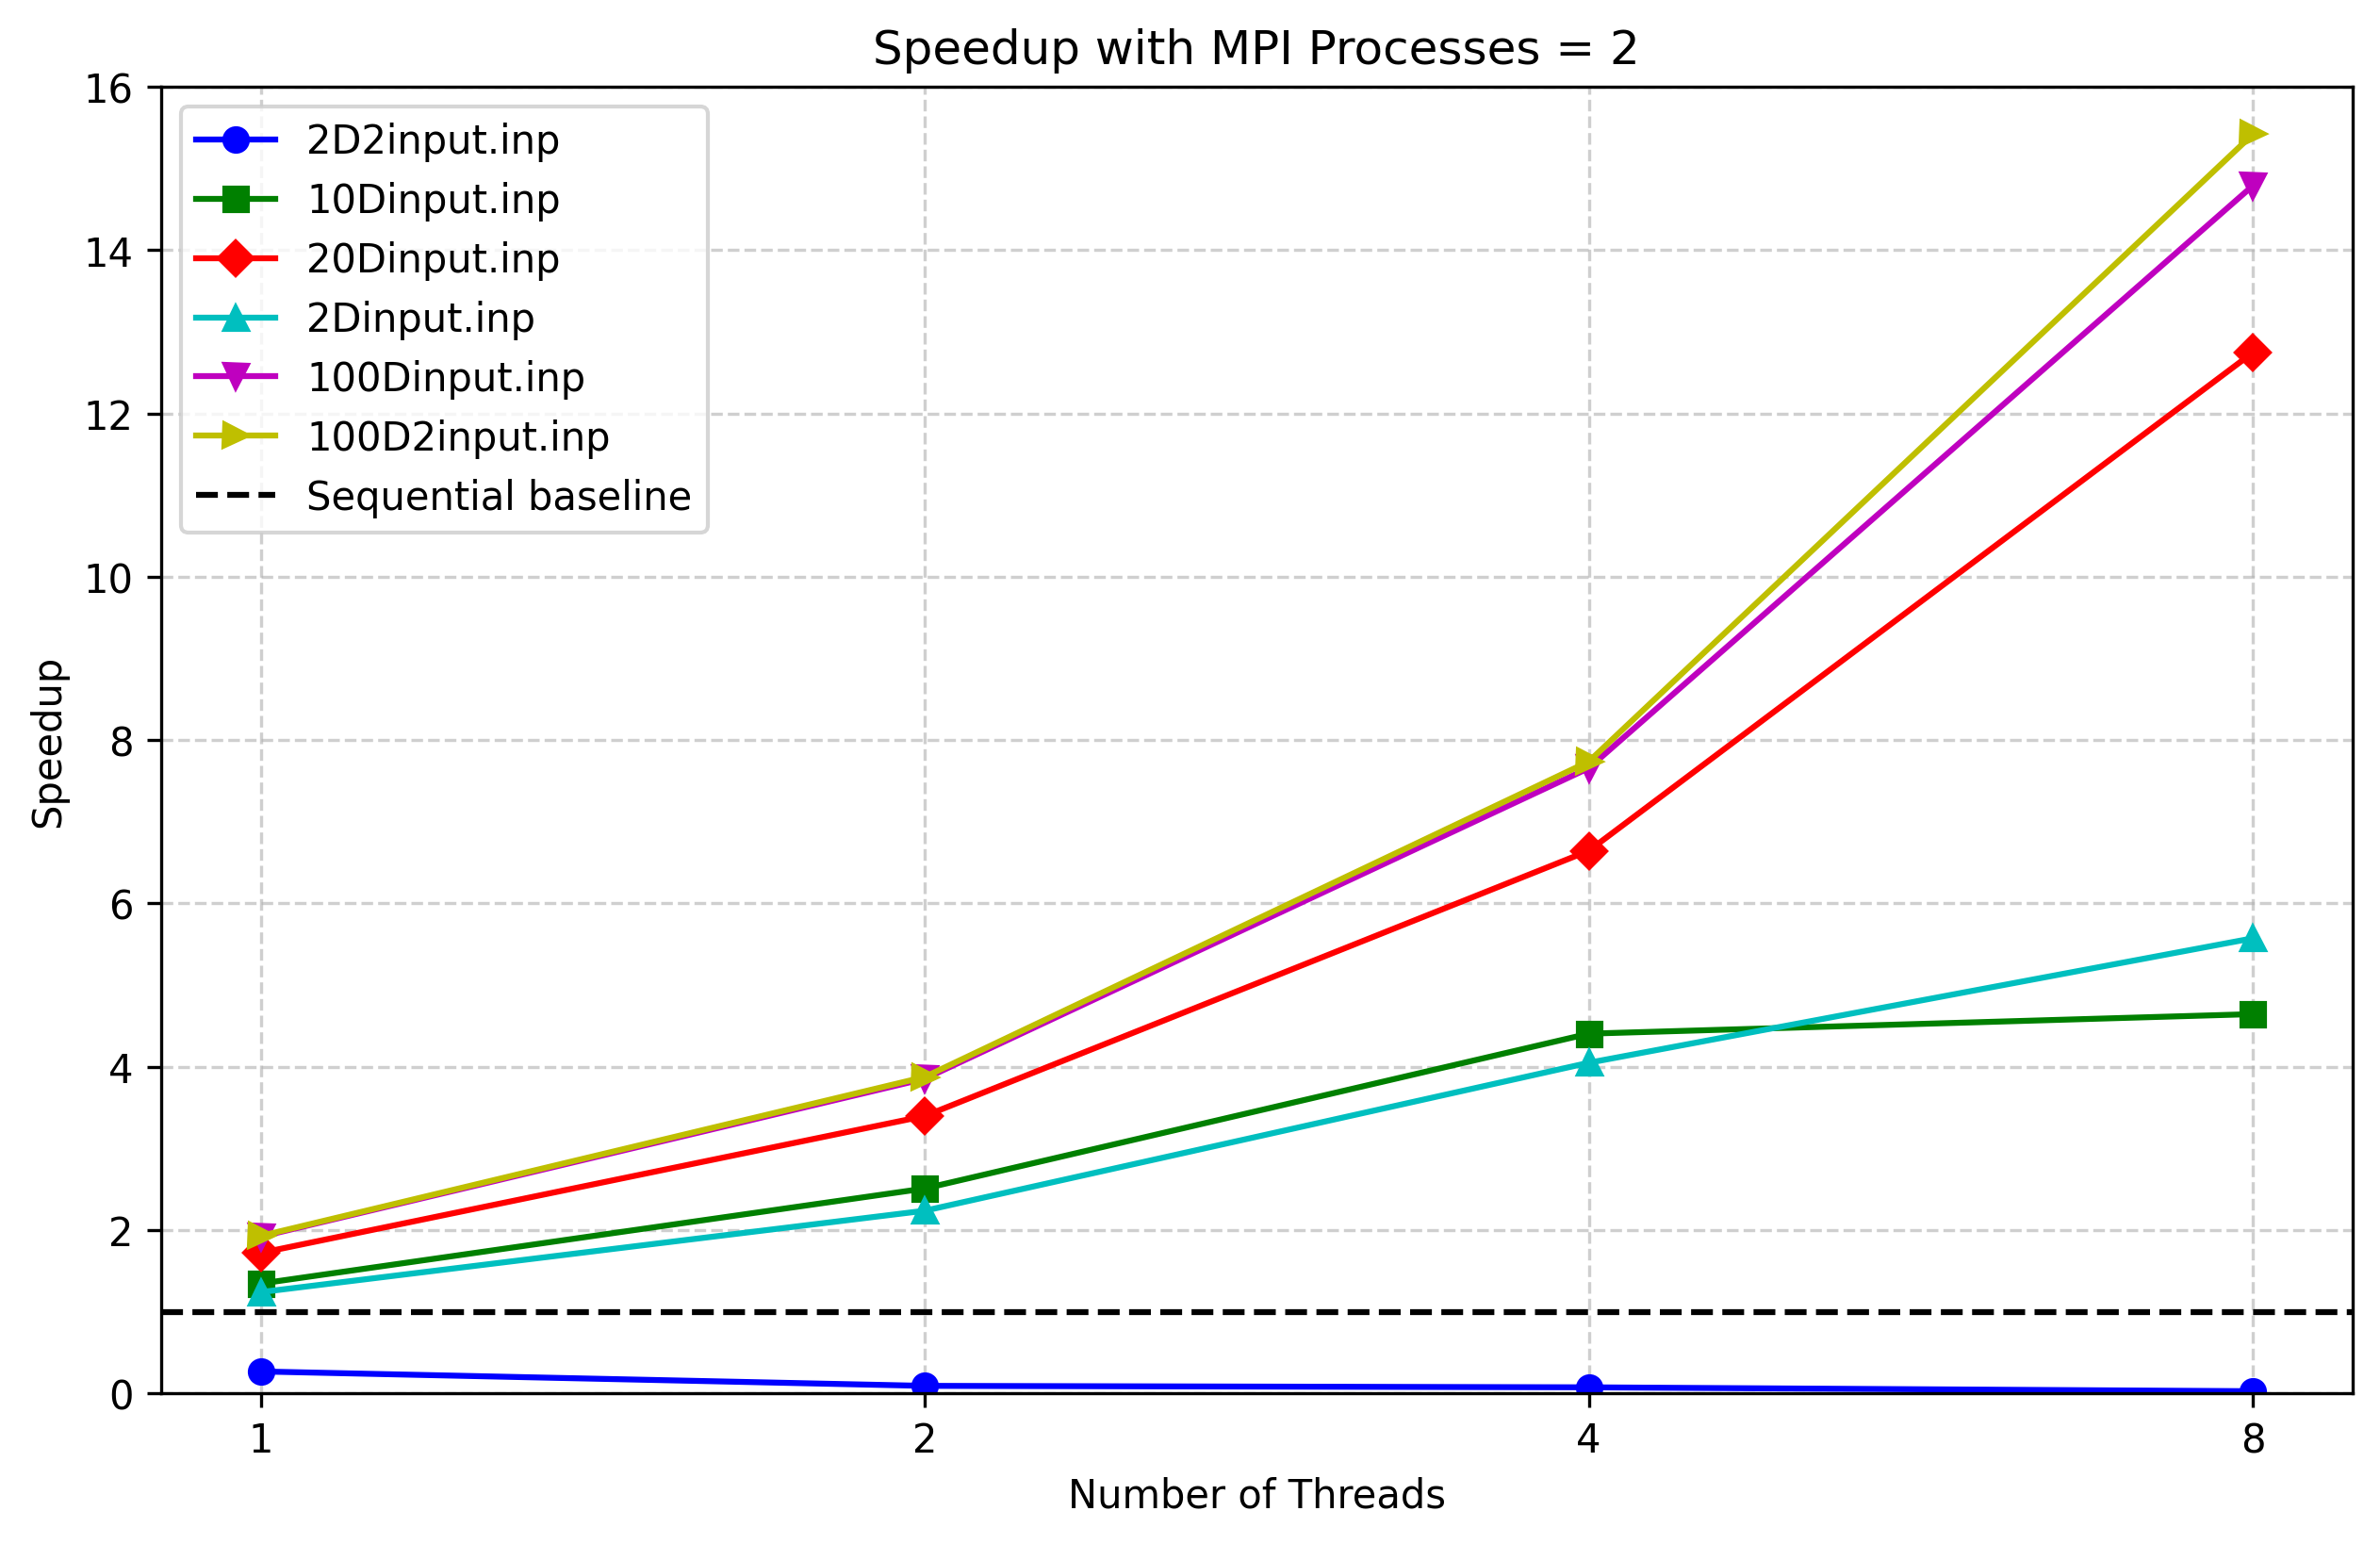
\includegraphics[width=\linewidth]{../test_csv/plots/speedup/plot_omp_mpi_2_small_slurm.png}
    \end{minipage}
    \begin{minipage}{0.4\textwidth}
      \centering
      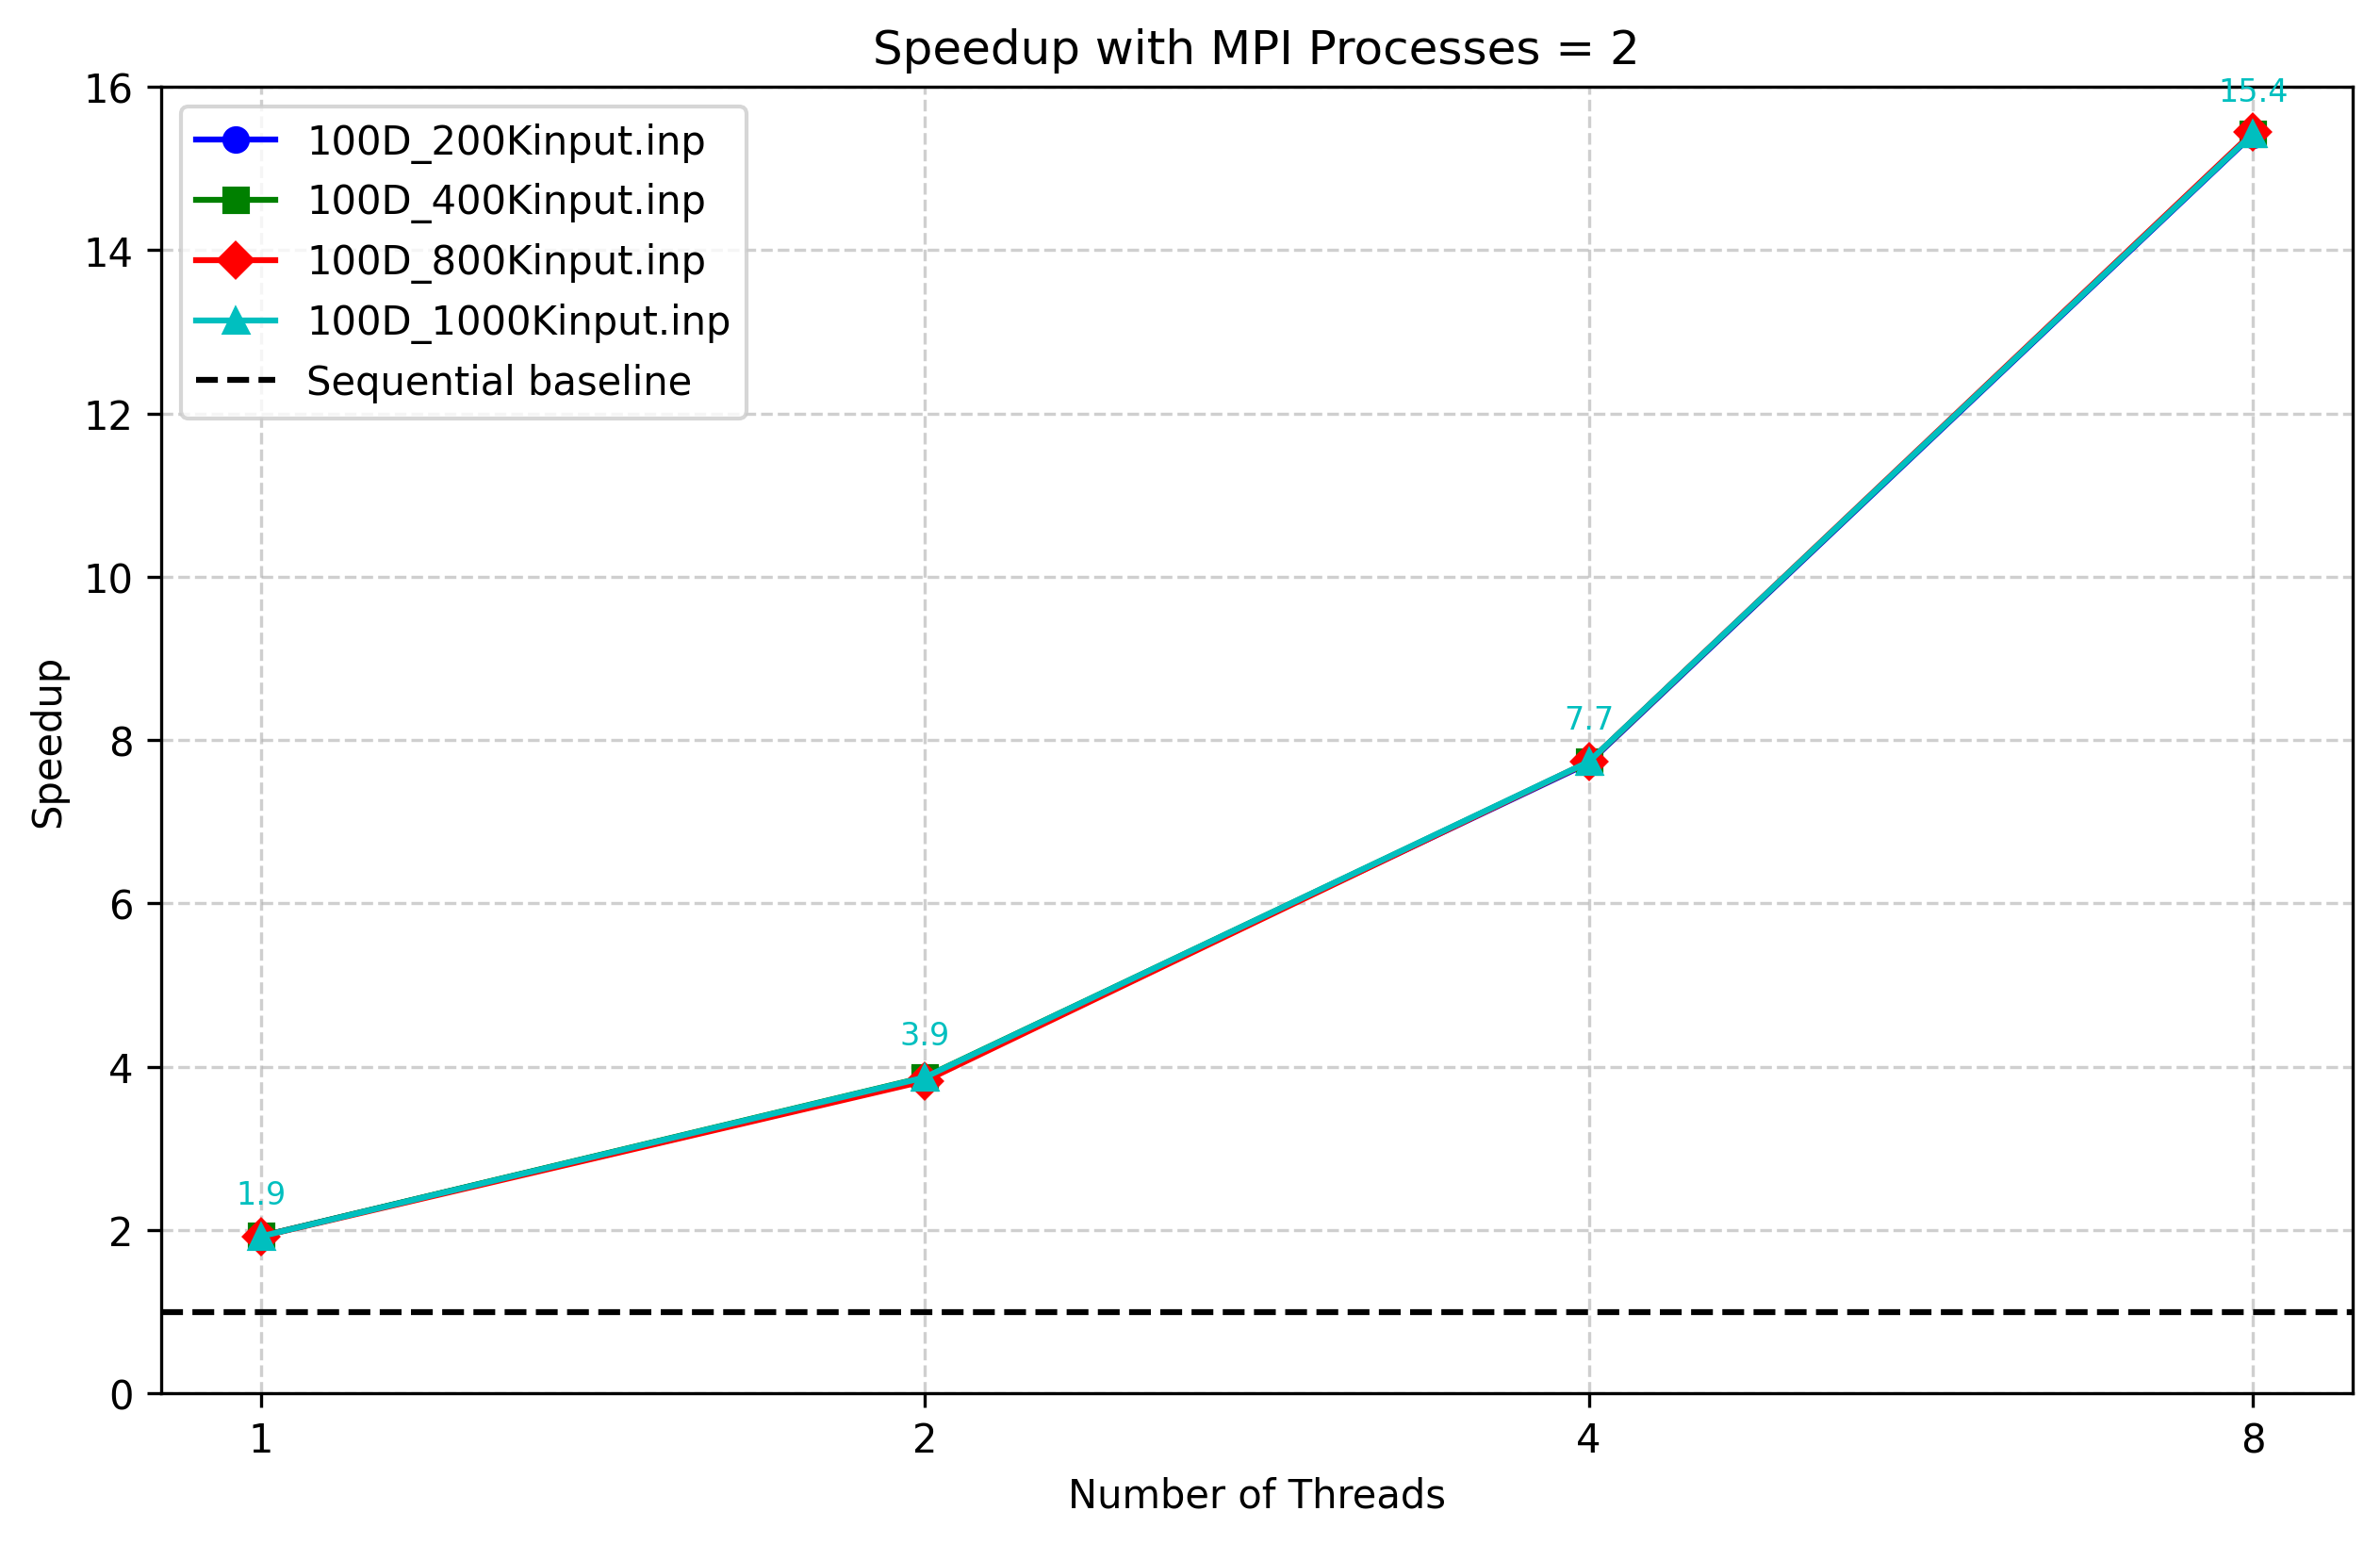
\includegraphics[width=\linewidth]{../test_csv/plots/speedup/plot_omp_mpi_2_big_slurm.png}
    \end{minipage}
    \begin{minipage}{0.4\textwidth}
      \centering
      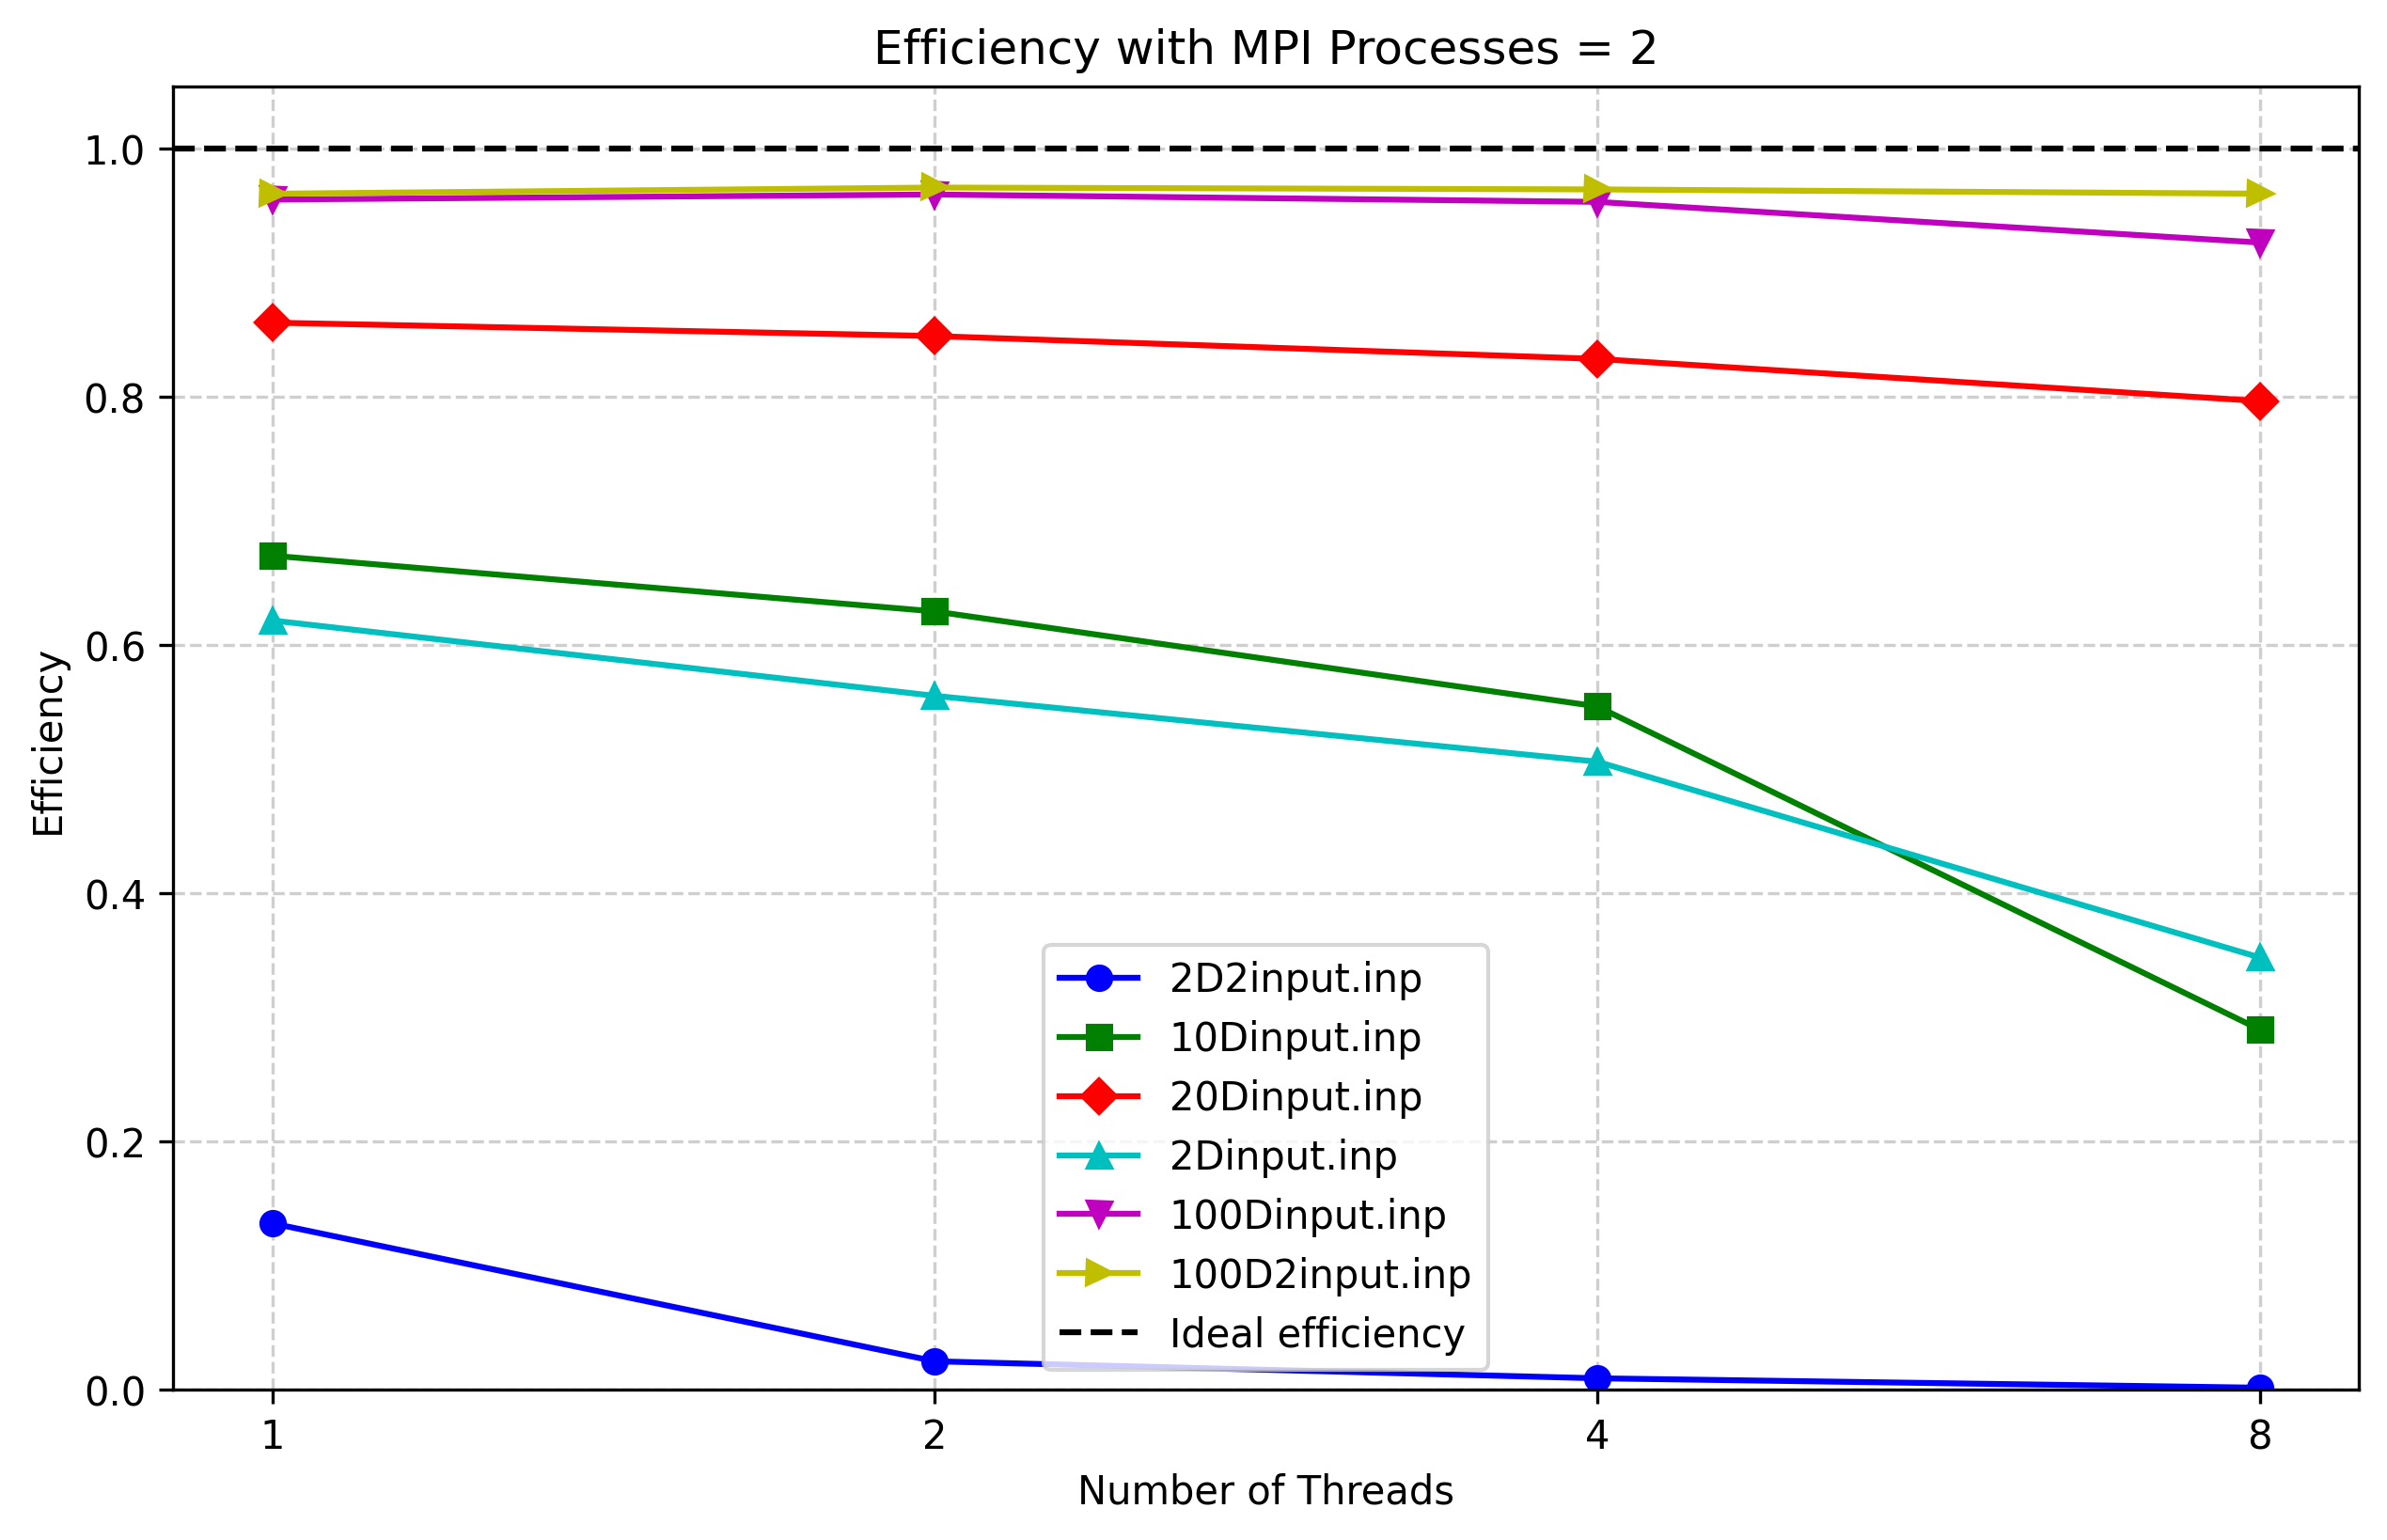
\includegraphics[width=\linewidth]{../test_csv/plots/efficency/plot_omp_mpi_2_small_slurm.png}
    \end{minipage}
    \begin{minipage}{0.4\textwidth}
      \centering
      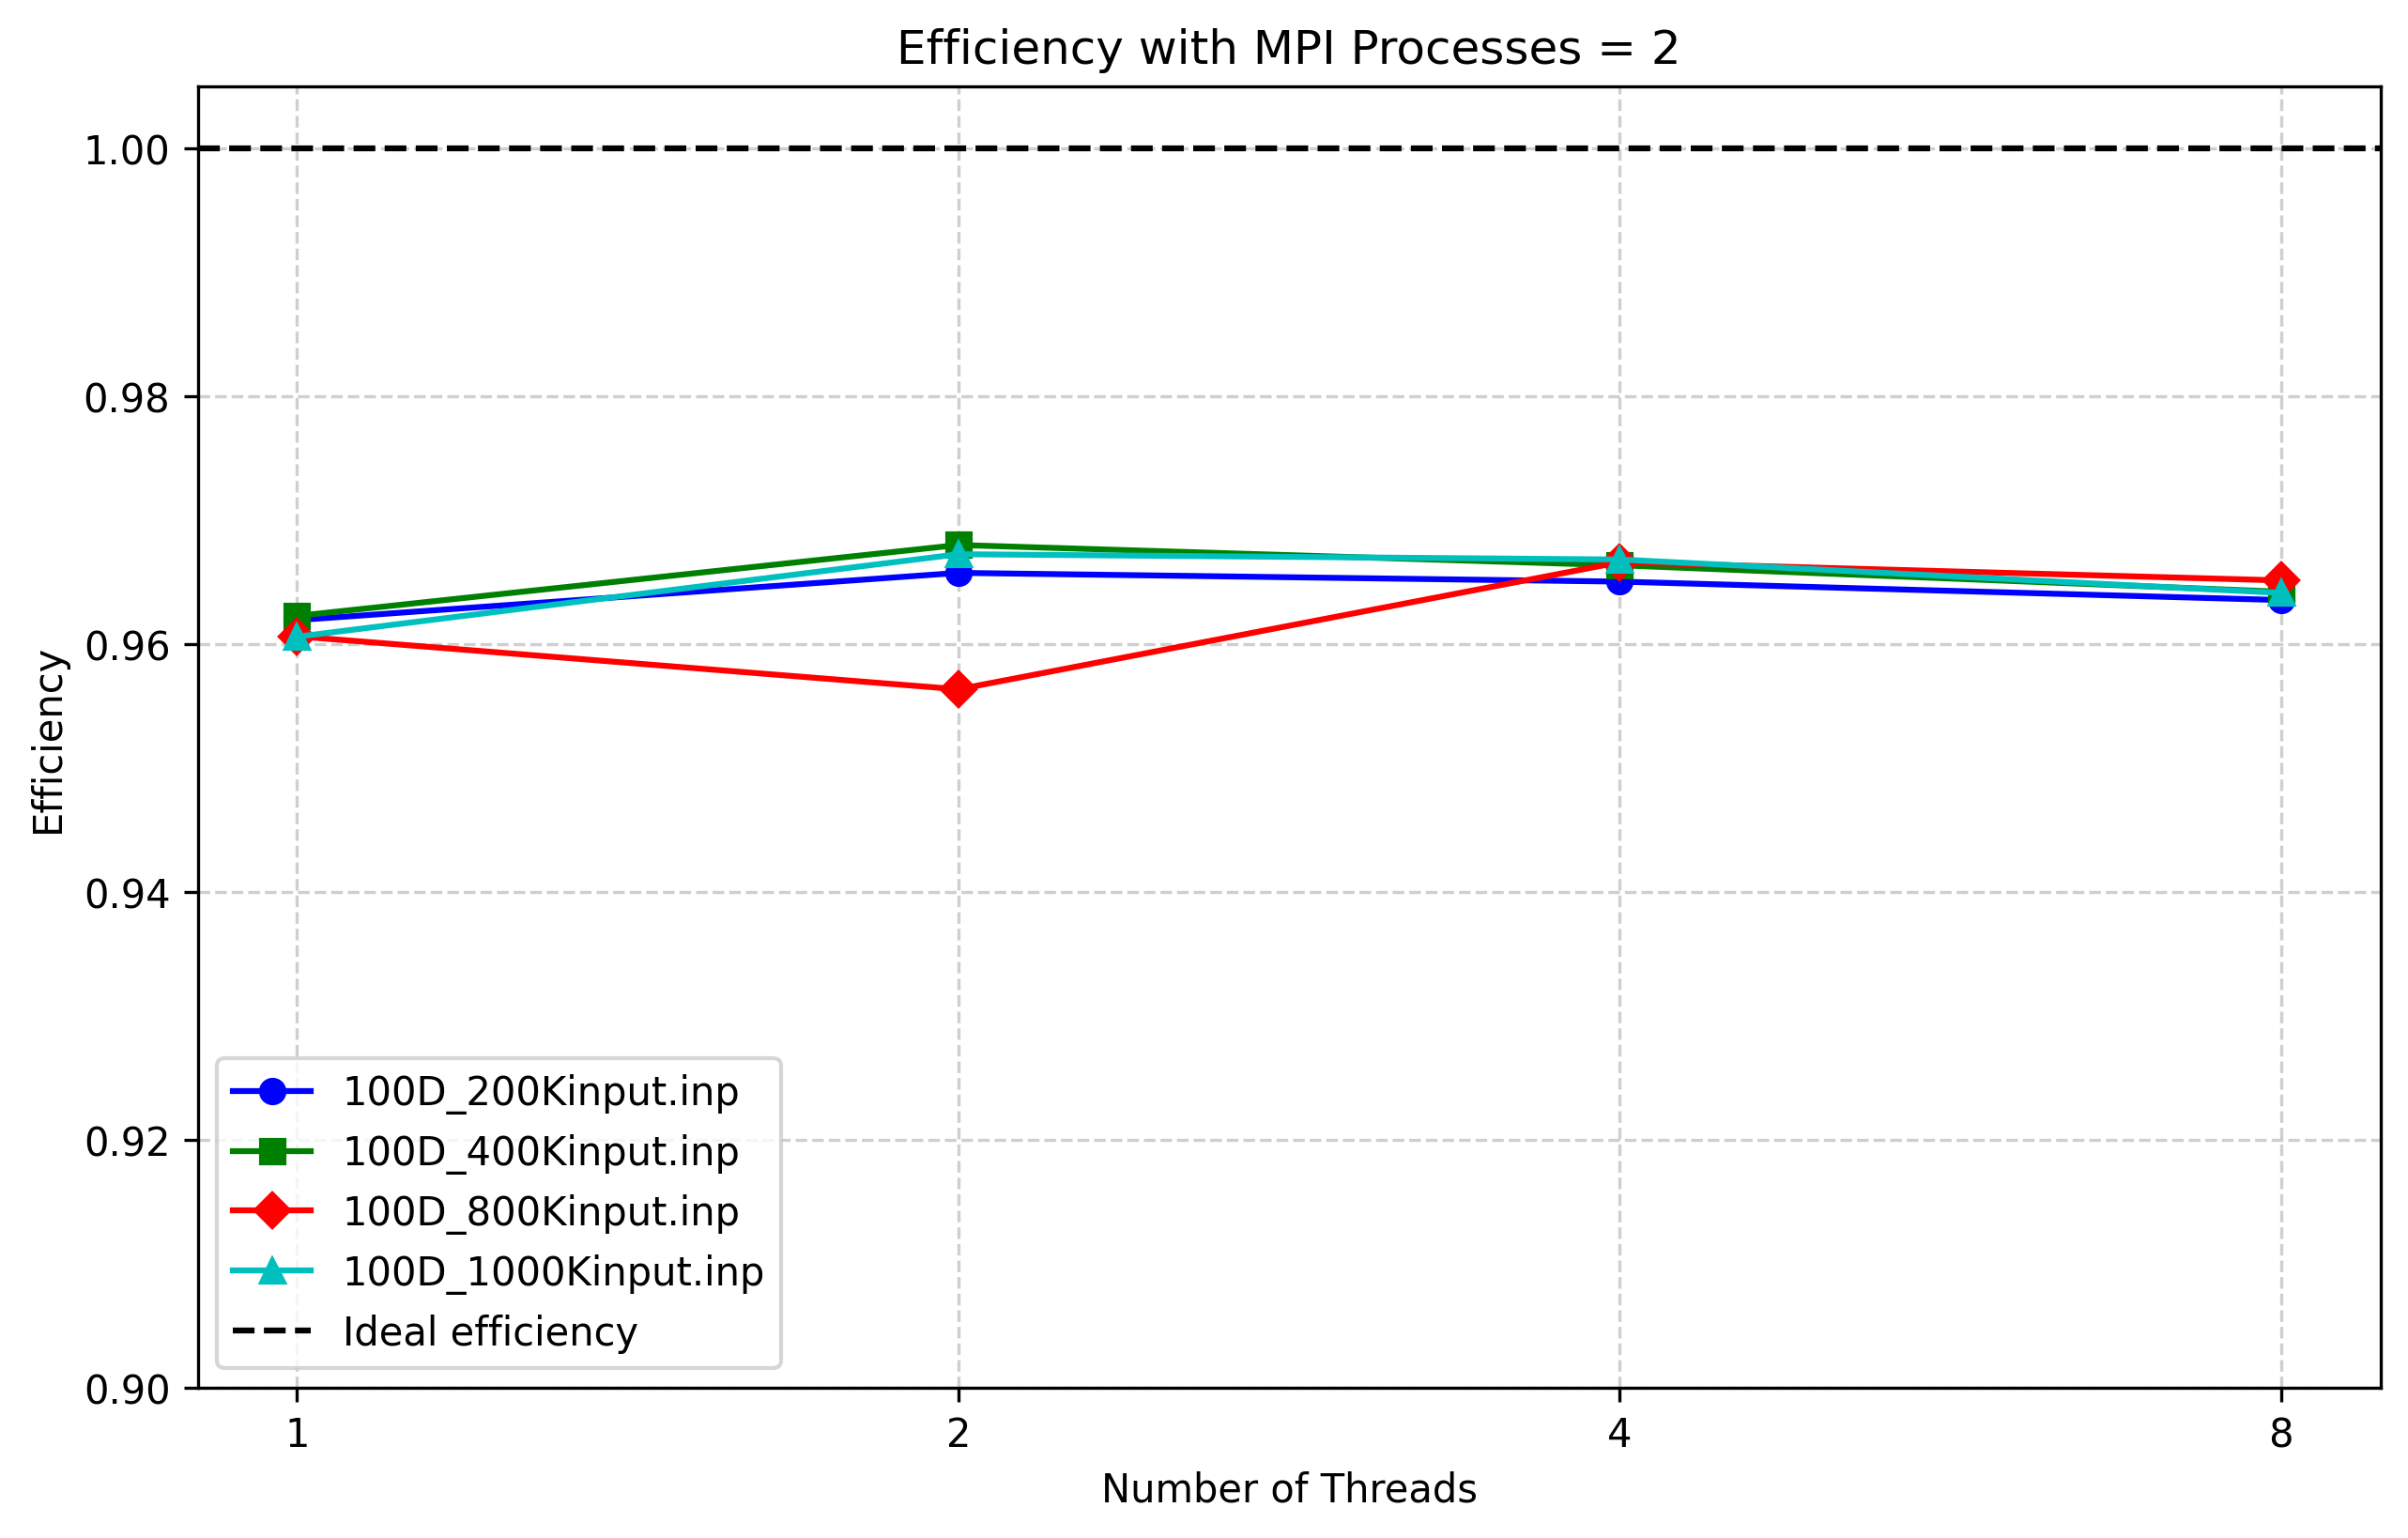
\includegraphics[width=\linewidth]{../test_csv/plots/efficency/plot_omp_mpi_2_big_slurm.png}
    \end{minipage}
  \end{figure}
  Per ogni test notiamo che ci sono delle differenze, ovvero, se prendiamo i test leggeri, aumentando il numero di thread
  lo speedup va ad aumentare, tuttavia il valore rimane basso, mentre sui test grandi lo speedup va ad aumentare diventando quasi uno
  speedup lineare. Notiamo anche, che all'aumentare della pesantezza 
  dei test e all'aumentare dei thread, lo speedup rimane più o meno costante.

  Per quanto riguarda l'efficenza, possiamo fare lo stesso discorso che abbiamo fatto con lo speedup, infatti sui test leggeri l'efficenza va a diminuire all'aumentare del 
  numero di thread, mentre rimane alta sui test pesanti. Invece, all'aumentare della grandezza dei test e all'aumentare del numero di thread, l'efficenza rimane alta.

  \begin{center}
    \rule{2.5cm}{1pt} \makebox{\texttt{Test with 4 processes}} \rule{2.5cm}{1pt}
  \end{center}
  \begin{figure}[ht]
    \centering
    \begin{minipage}{0.4\textwidth}
      \centering
      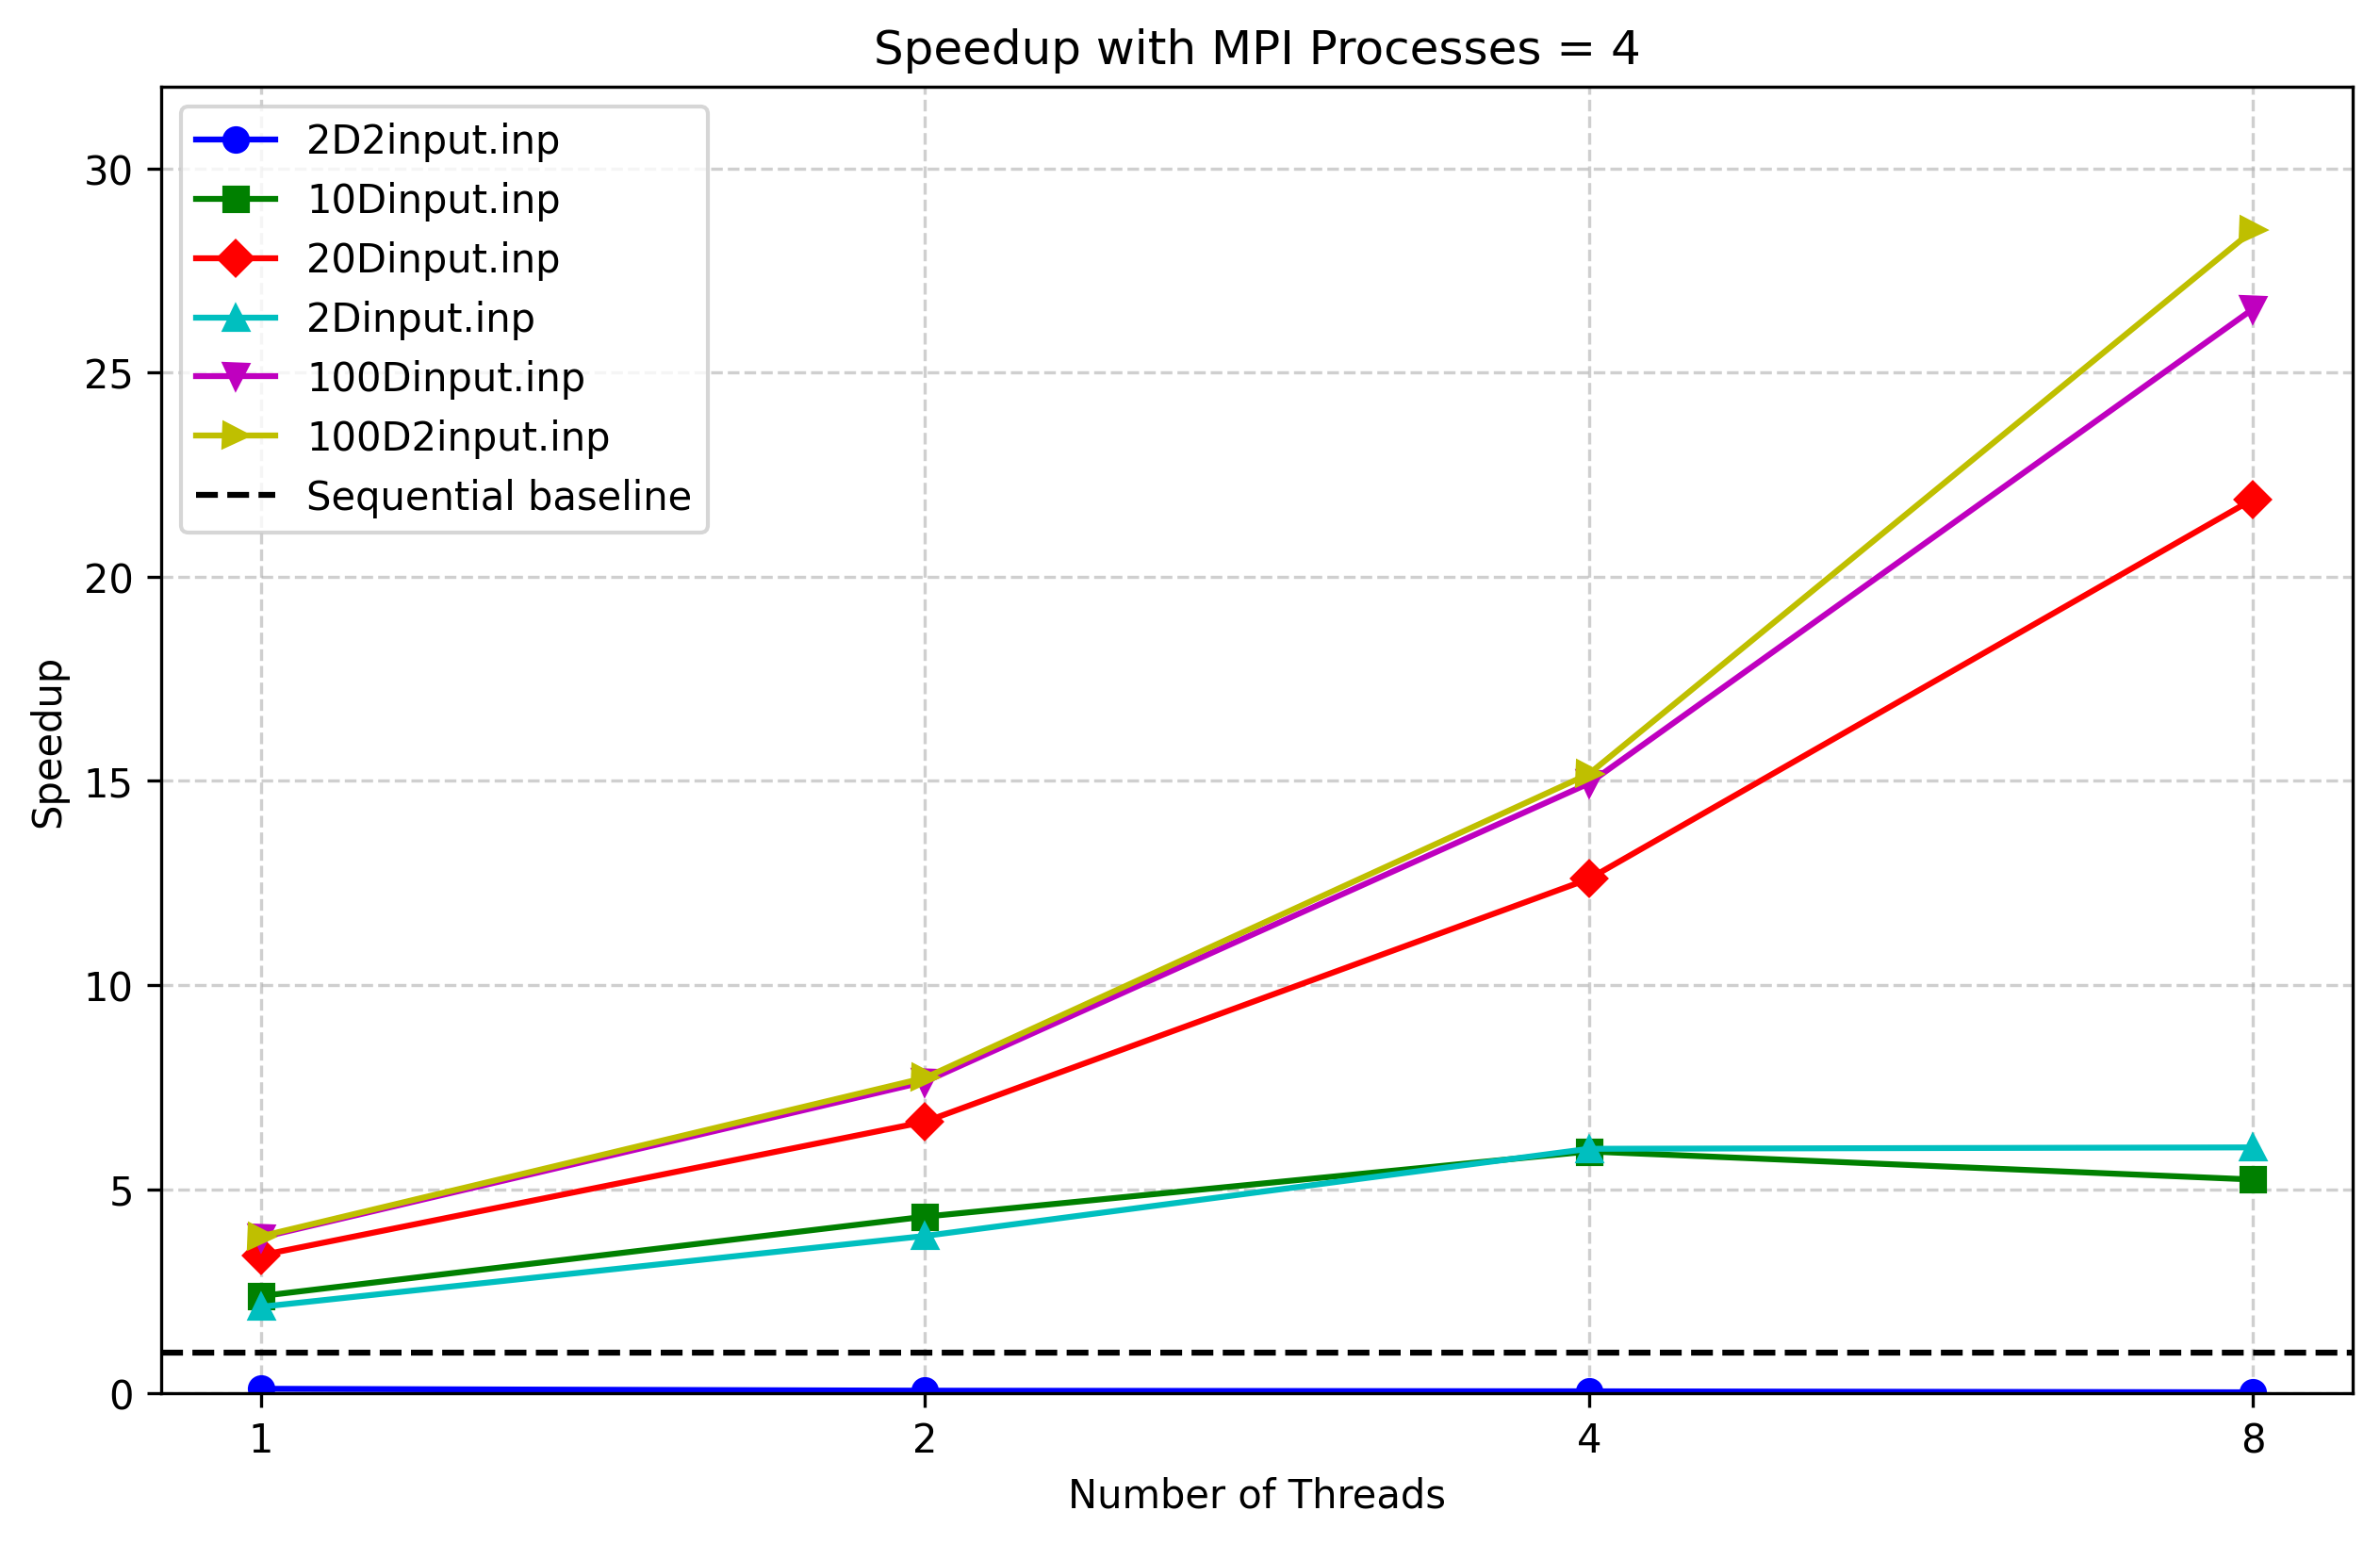
\includegraphics[width=\linewidth]{../test_csv/plots/speedup/plot_omp_mpi_4_small_slurm.png}
    \end{minipage}
    \begin{minipage}{0.4\textwidth}
      \centering
      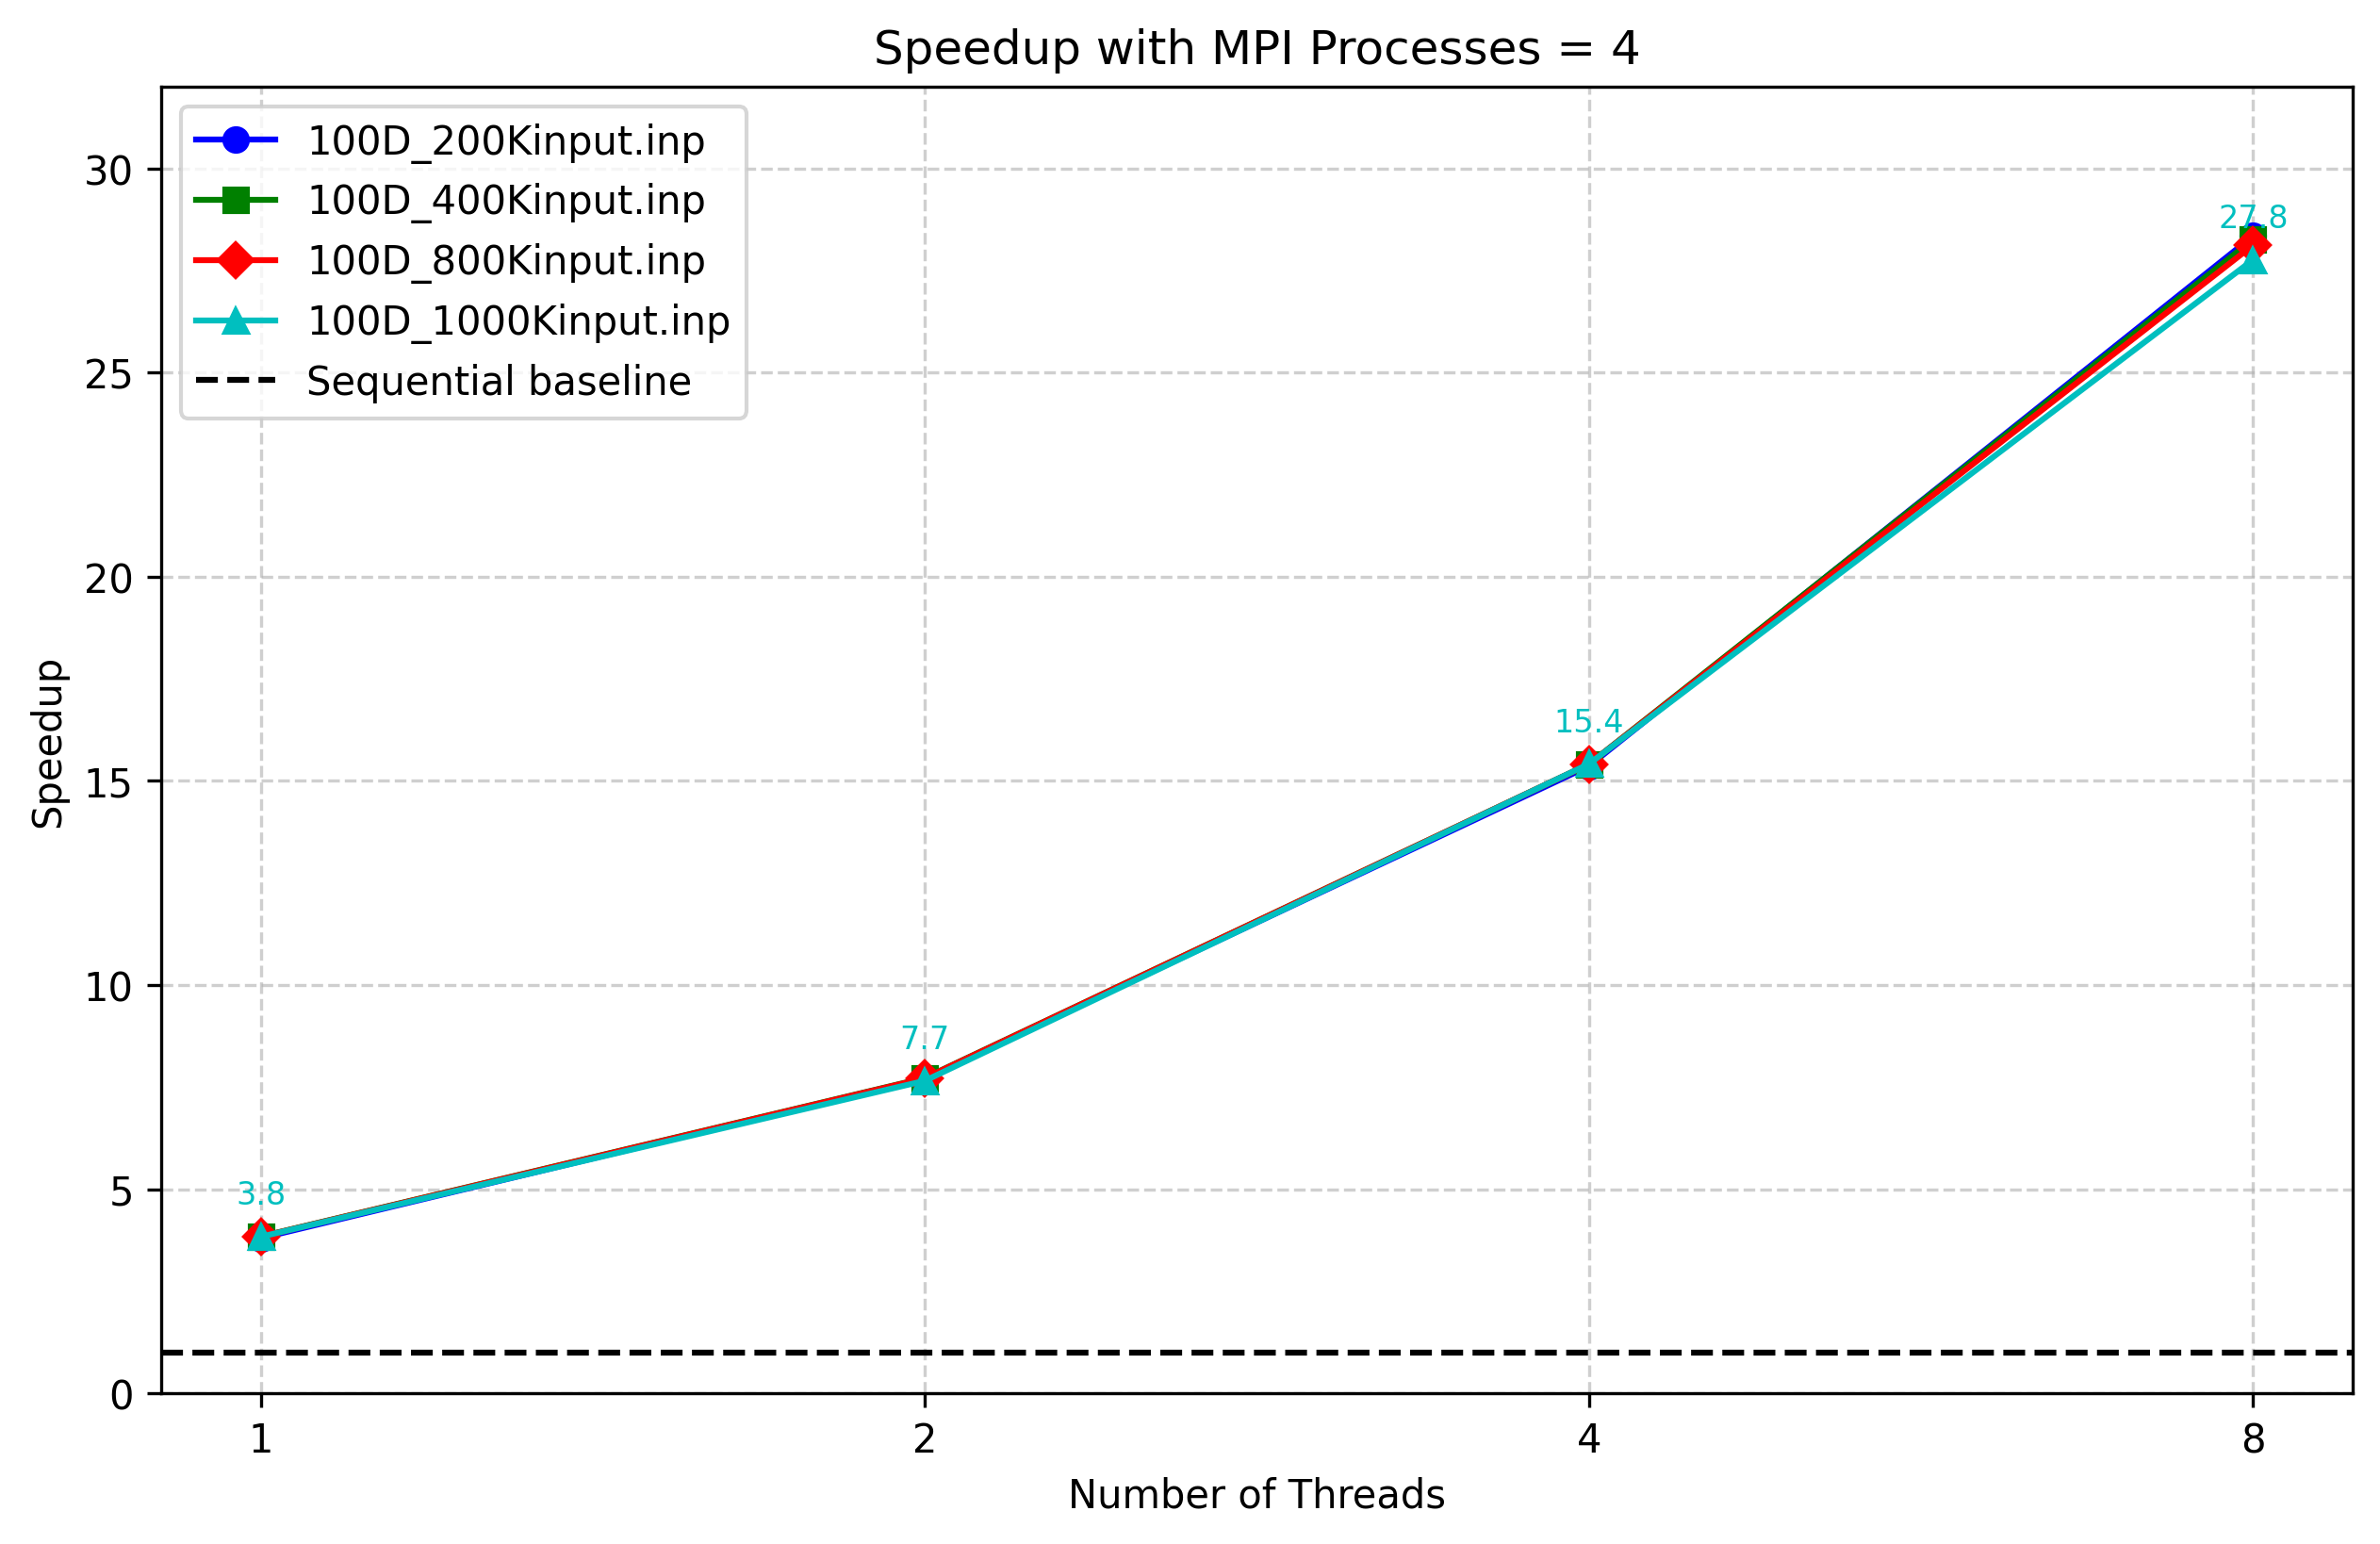
\includegraphics[width=\linewidth]{../test_csv/plots/speedup/plot_omp_mpi_4_big_slurm.png}
    \end{minipage}
    \begin{minipage}{0.4\textwidth}
      \centering
      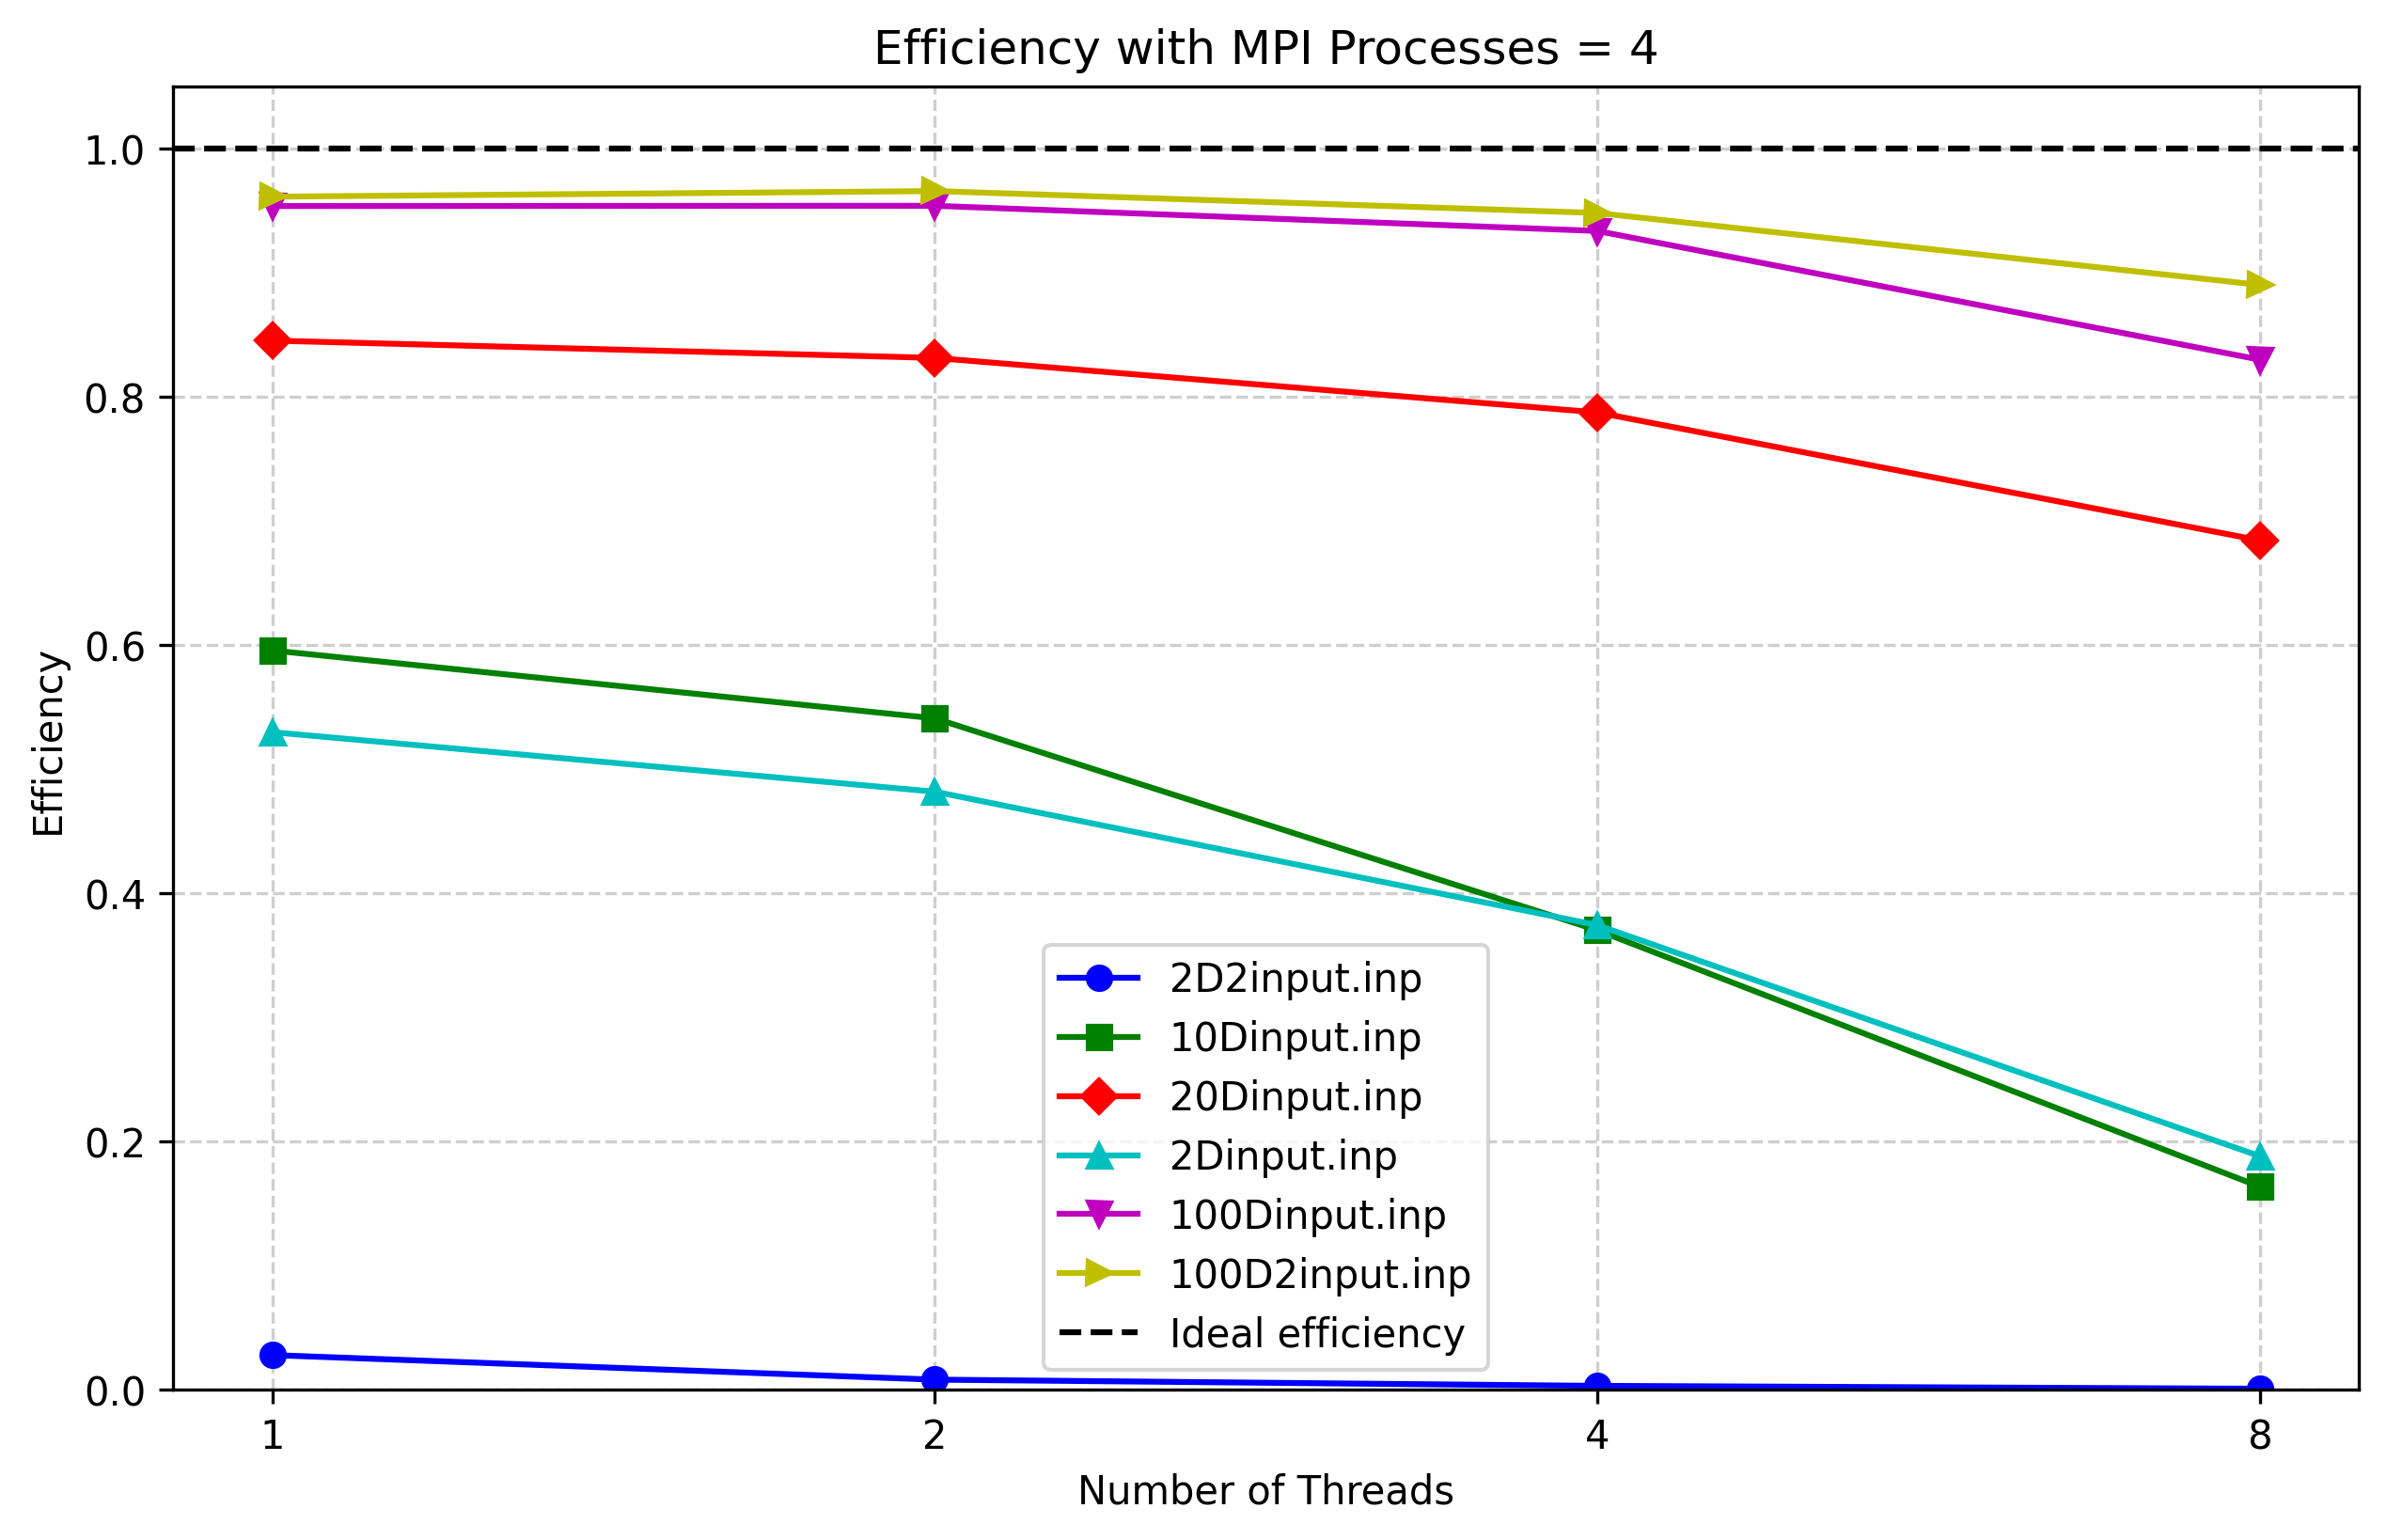
\includegraphics[width=\linewidth]{../test_csv/plots/efficency/plot_omp_mpi_4_small_slurm.png}
    \end{minipage}
    \begin{minipage}{0.4\textwidth}
      \centering
      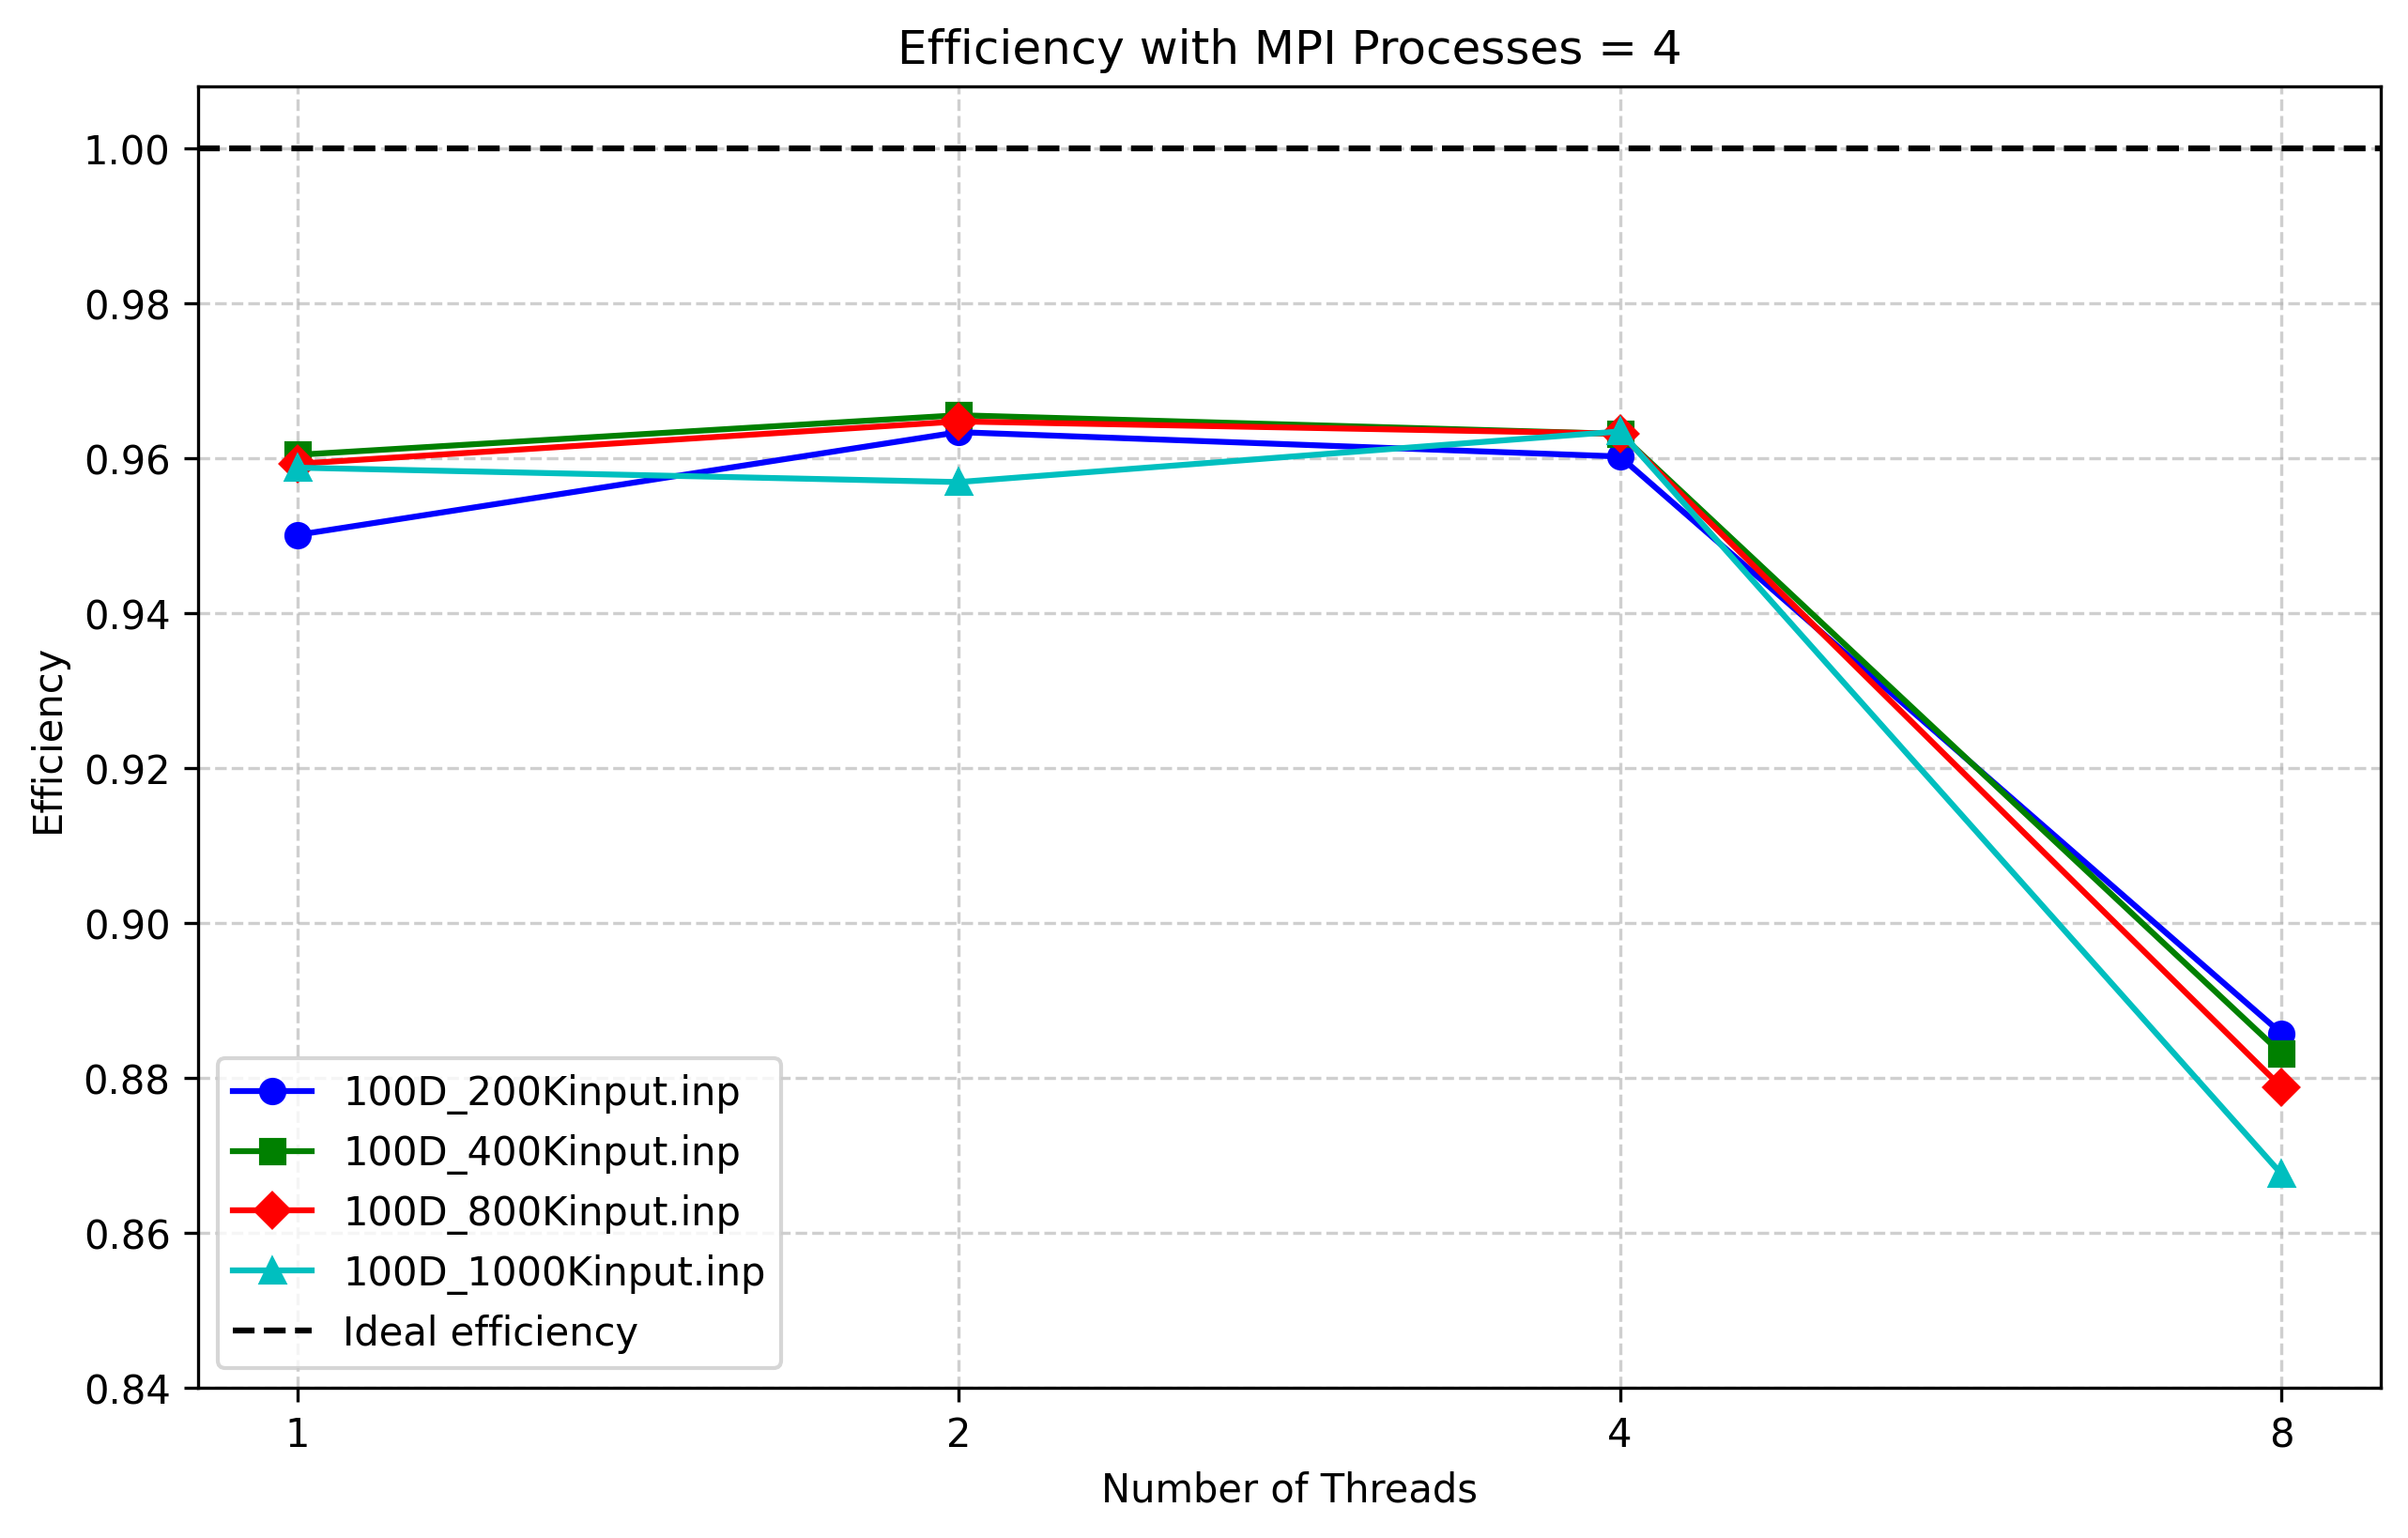
\includegraphics[width=\linewidth]{../test_csv/plots/efficency/plot_omp_mpi_4_big_slurm.png}
    \end{minipage}
  \end{figure}

  Una principale differenza che notiamo è che nei test con 2 processi, con i file input più leggeri hanno uno speedup molto basso fino ad essere più lenti del sequenziale (nel caso del file input 2D2) di conseguenza hanno anche un'efficenza molto bassa, ma 
  notiamo anche una differenza sui test pesanti, in quanto all'inzio con pochi thread i test mantengono uno speedup e un'efficenza alta, vicina a quella ideale, ma all'aumentare dei thread notiamo che lo speedup ha un margine di crescita 
  sempre più basso, mentre l'efficenza si abbassa, questo è dovuto al fatto che aumentando i processi e la mole di dati da elaborare, di conseguenza, l'overhead di comunicazione tra processi e il continuo accesso alla memoria 
  per l'elaborazione dei dati influisce molto nel tempo di esecuzione. Nonostante questo i valori mantenuti sono molto vicini a quelli ideali.
  
  \begin{center}
    \rule{2.5cm}{1pt} \makebox{\texttt{Test with 8 processes}} \rule{2.5cm}{1pt}
  \end{center}
  \begin{figure}[ht]
    \centering
    \begin{minipage}{0.4\textwidth}
      \centering
      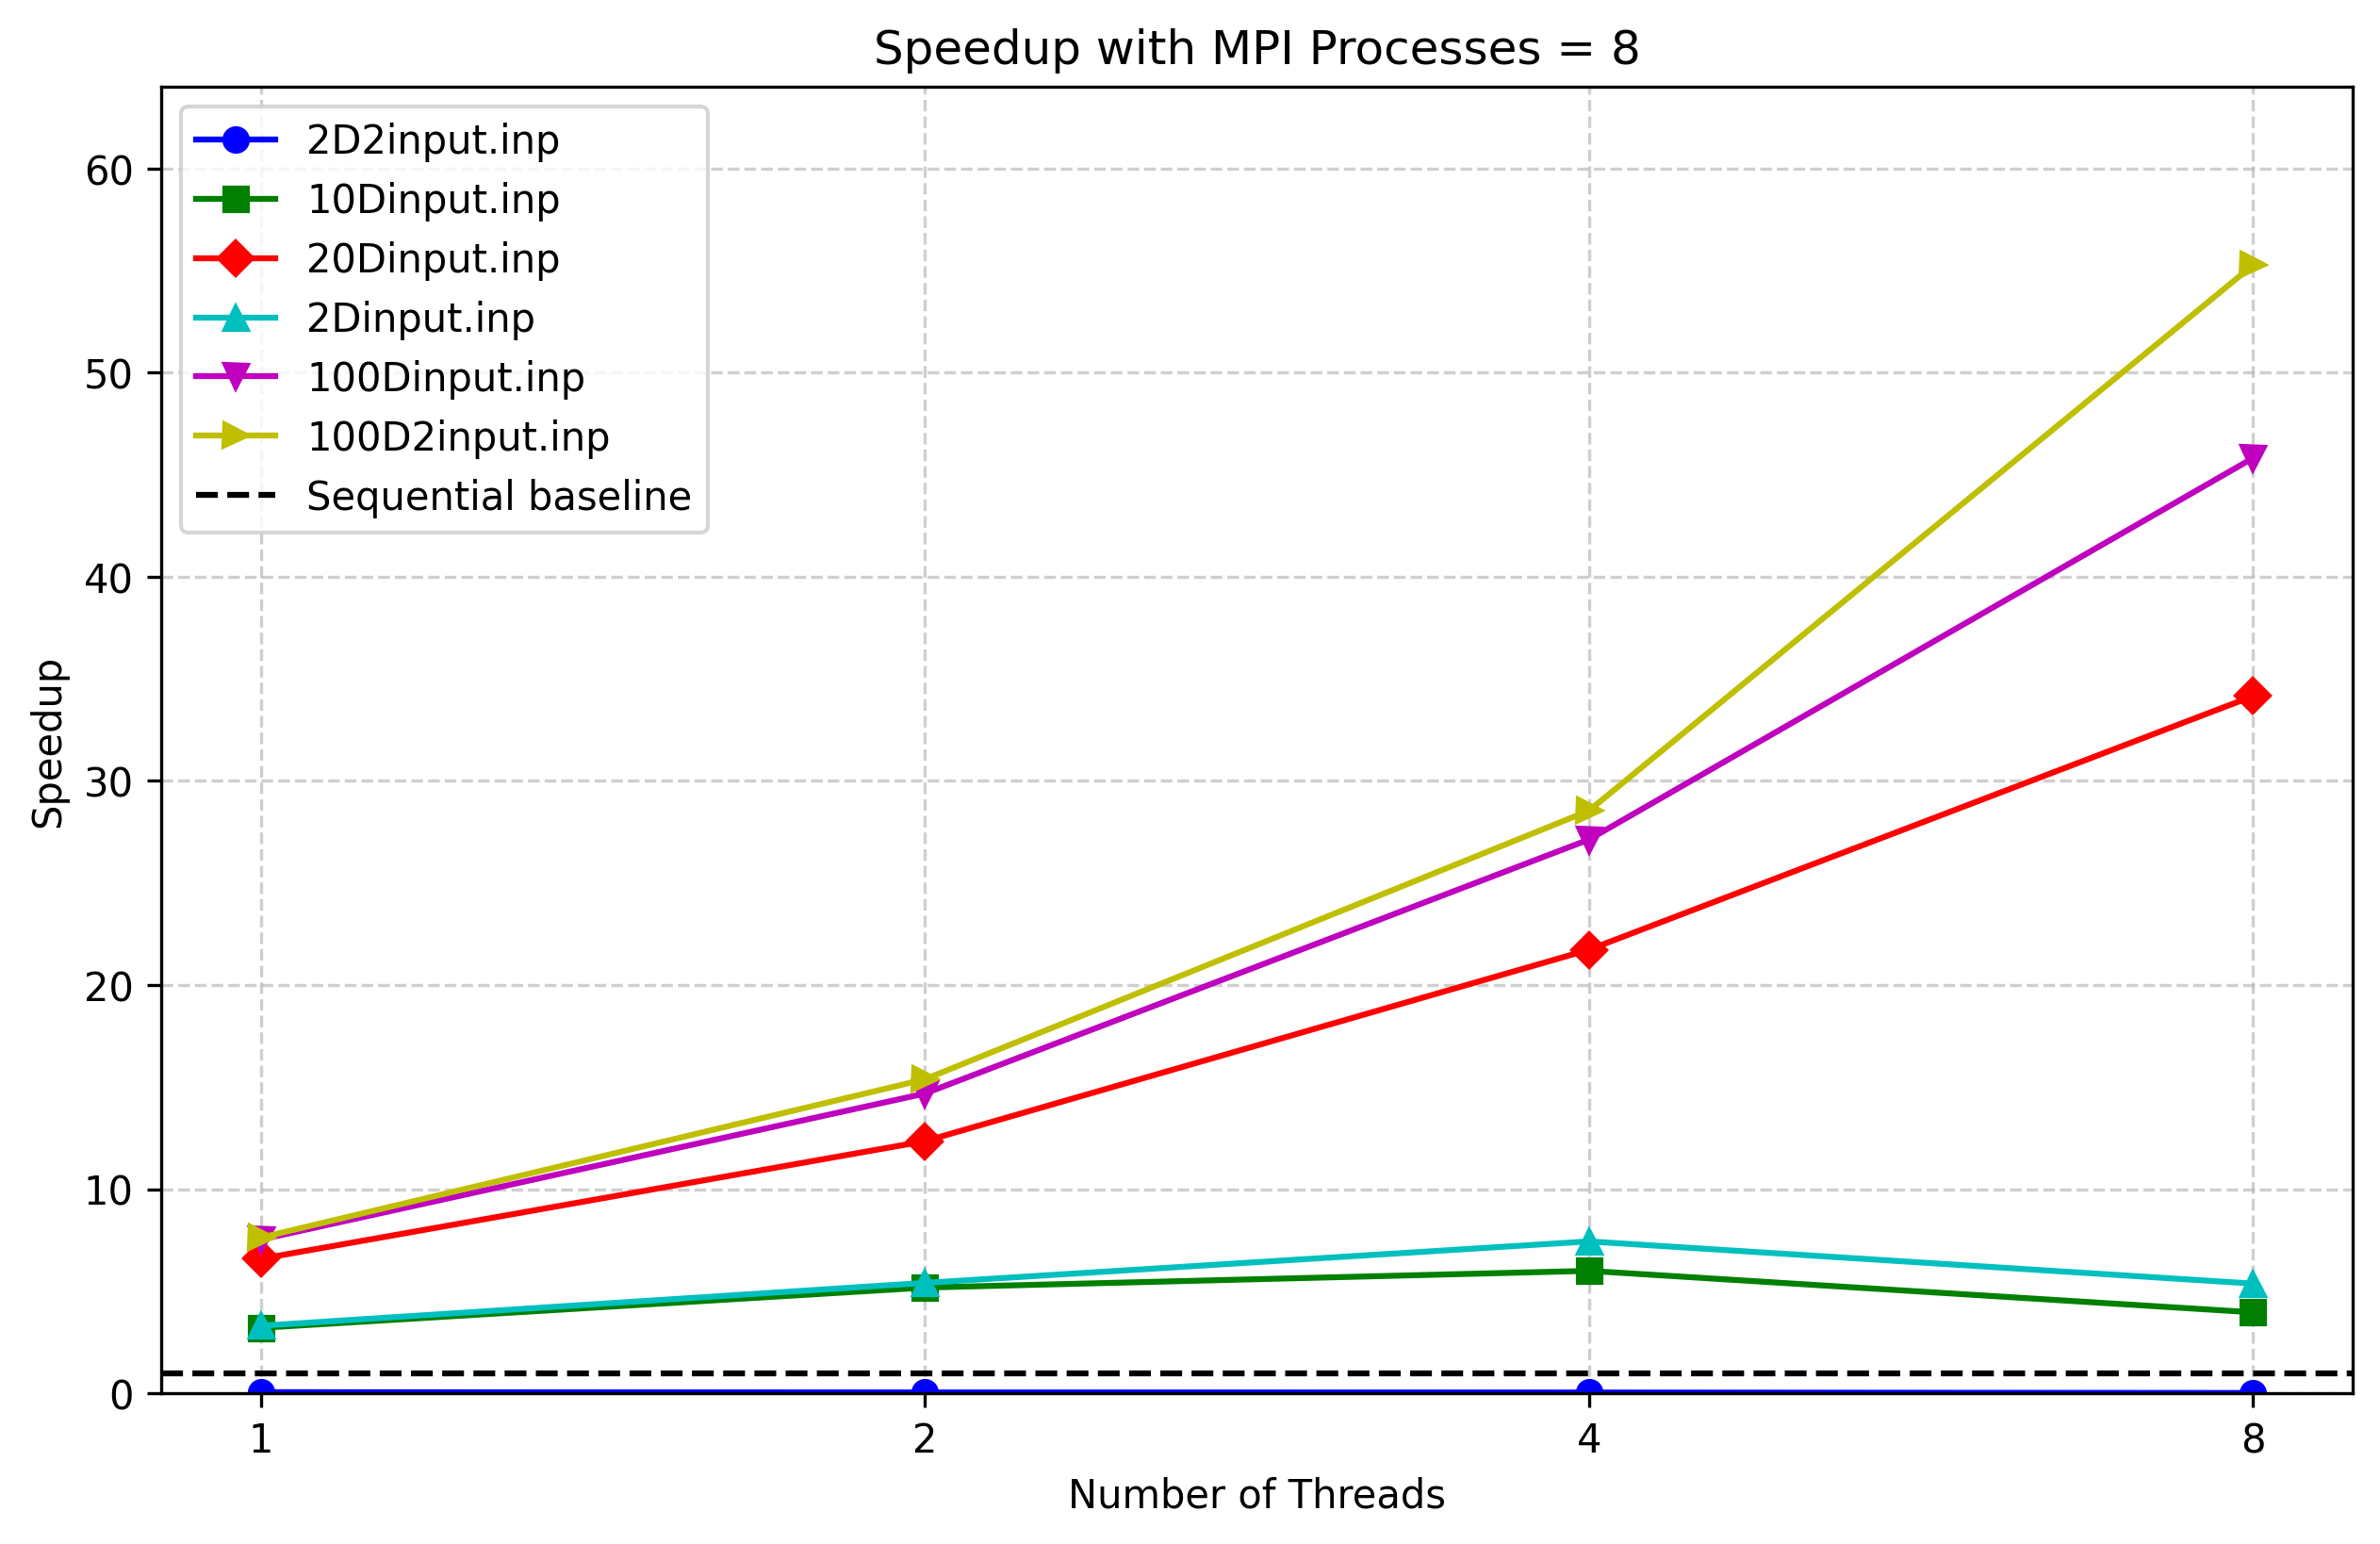
\includegraphics[width=\linewidth]{../test_csv/plots/speedup/plot_omp_mpi_8_small_slurm.png}
    \end{minipage}
    \begin{minipage}{0.4\textwidth}
      \centering
      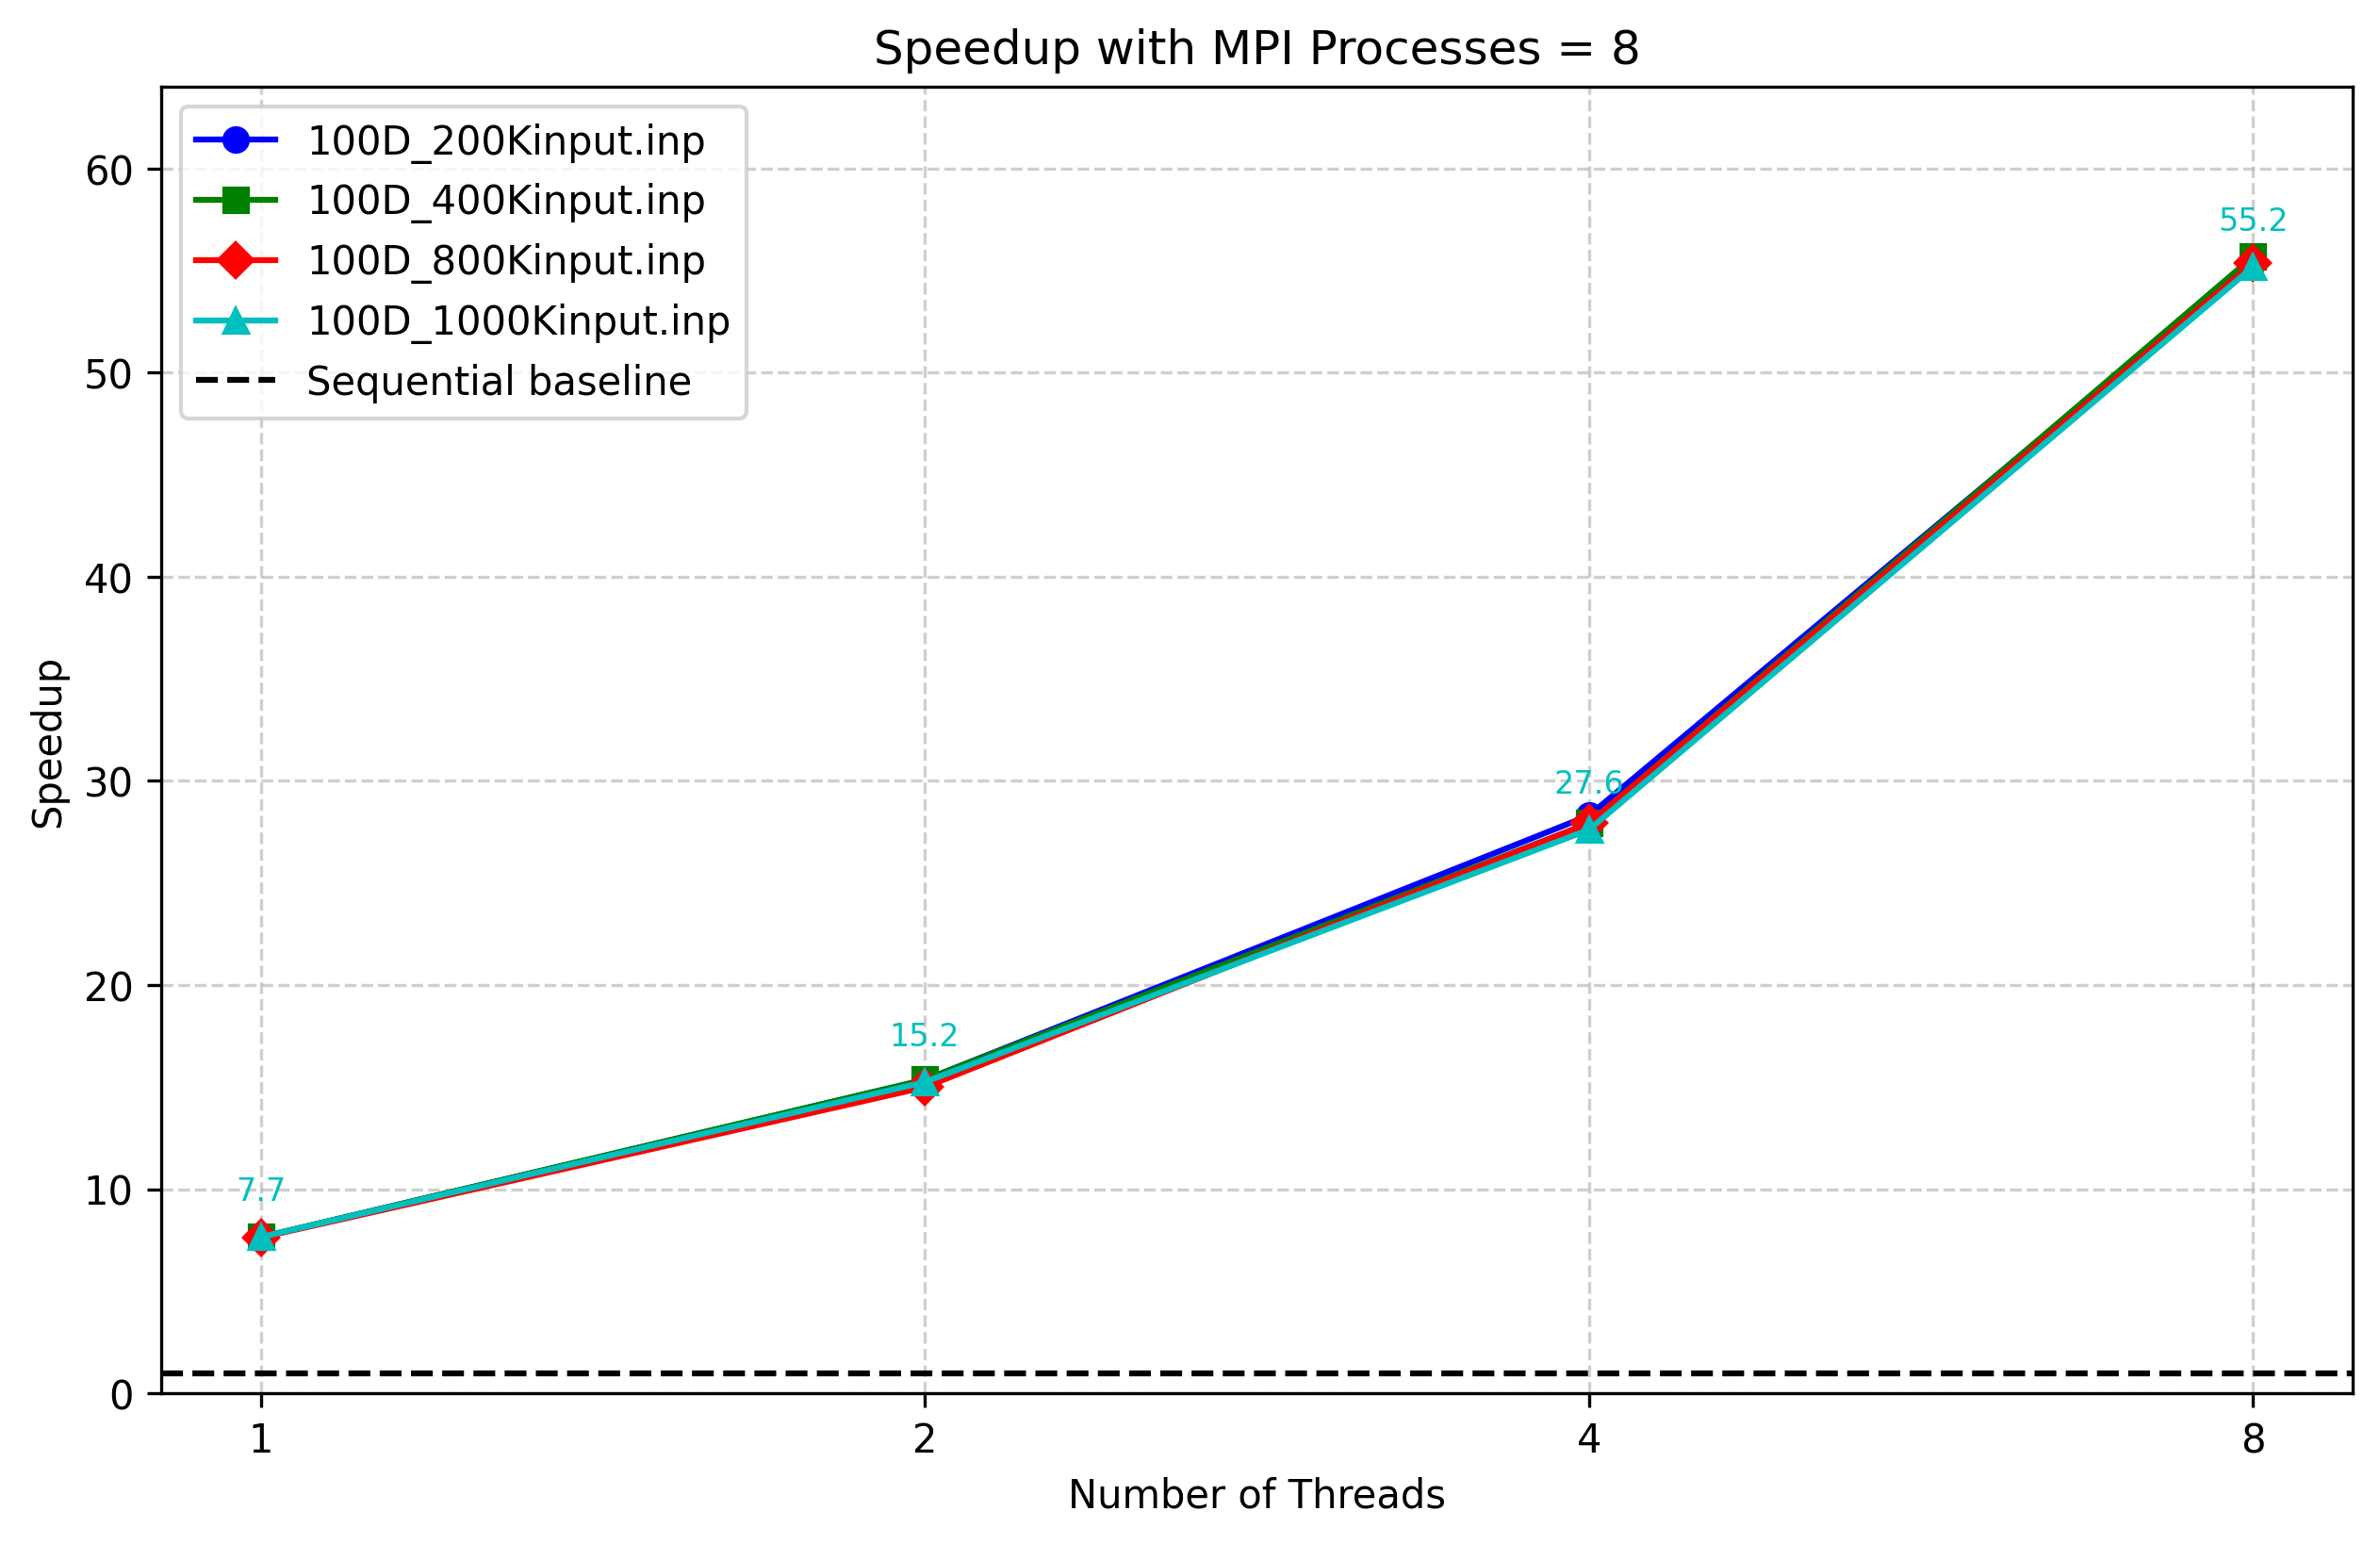
\includegraphics[width=\linewidth]{../test_csv/plots/speedup/plot_omp_mpi_8_big_slurm.png}
    \end{minipage}
    \begin{minipage}{0.4\textwidth}
      \centering
      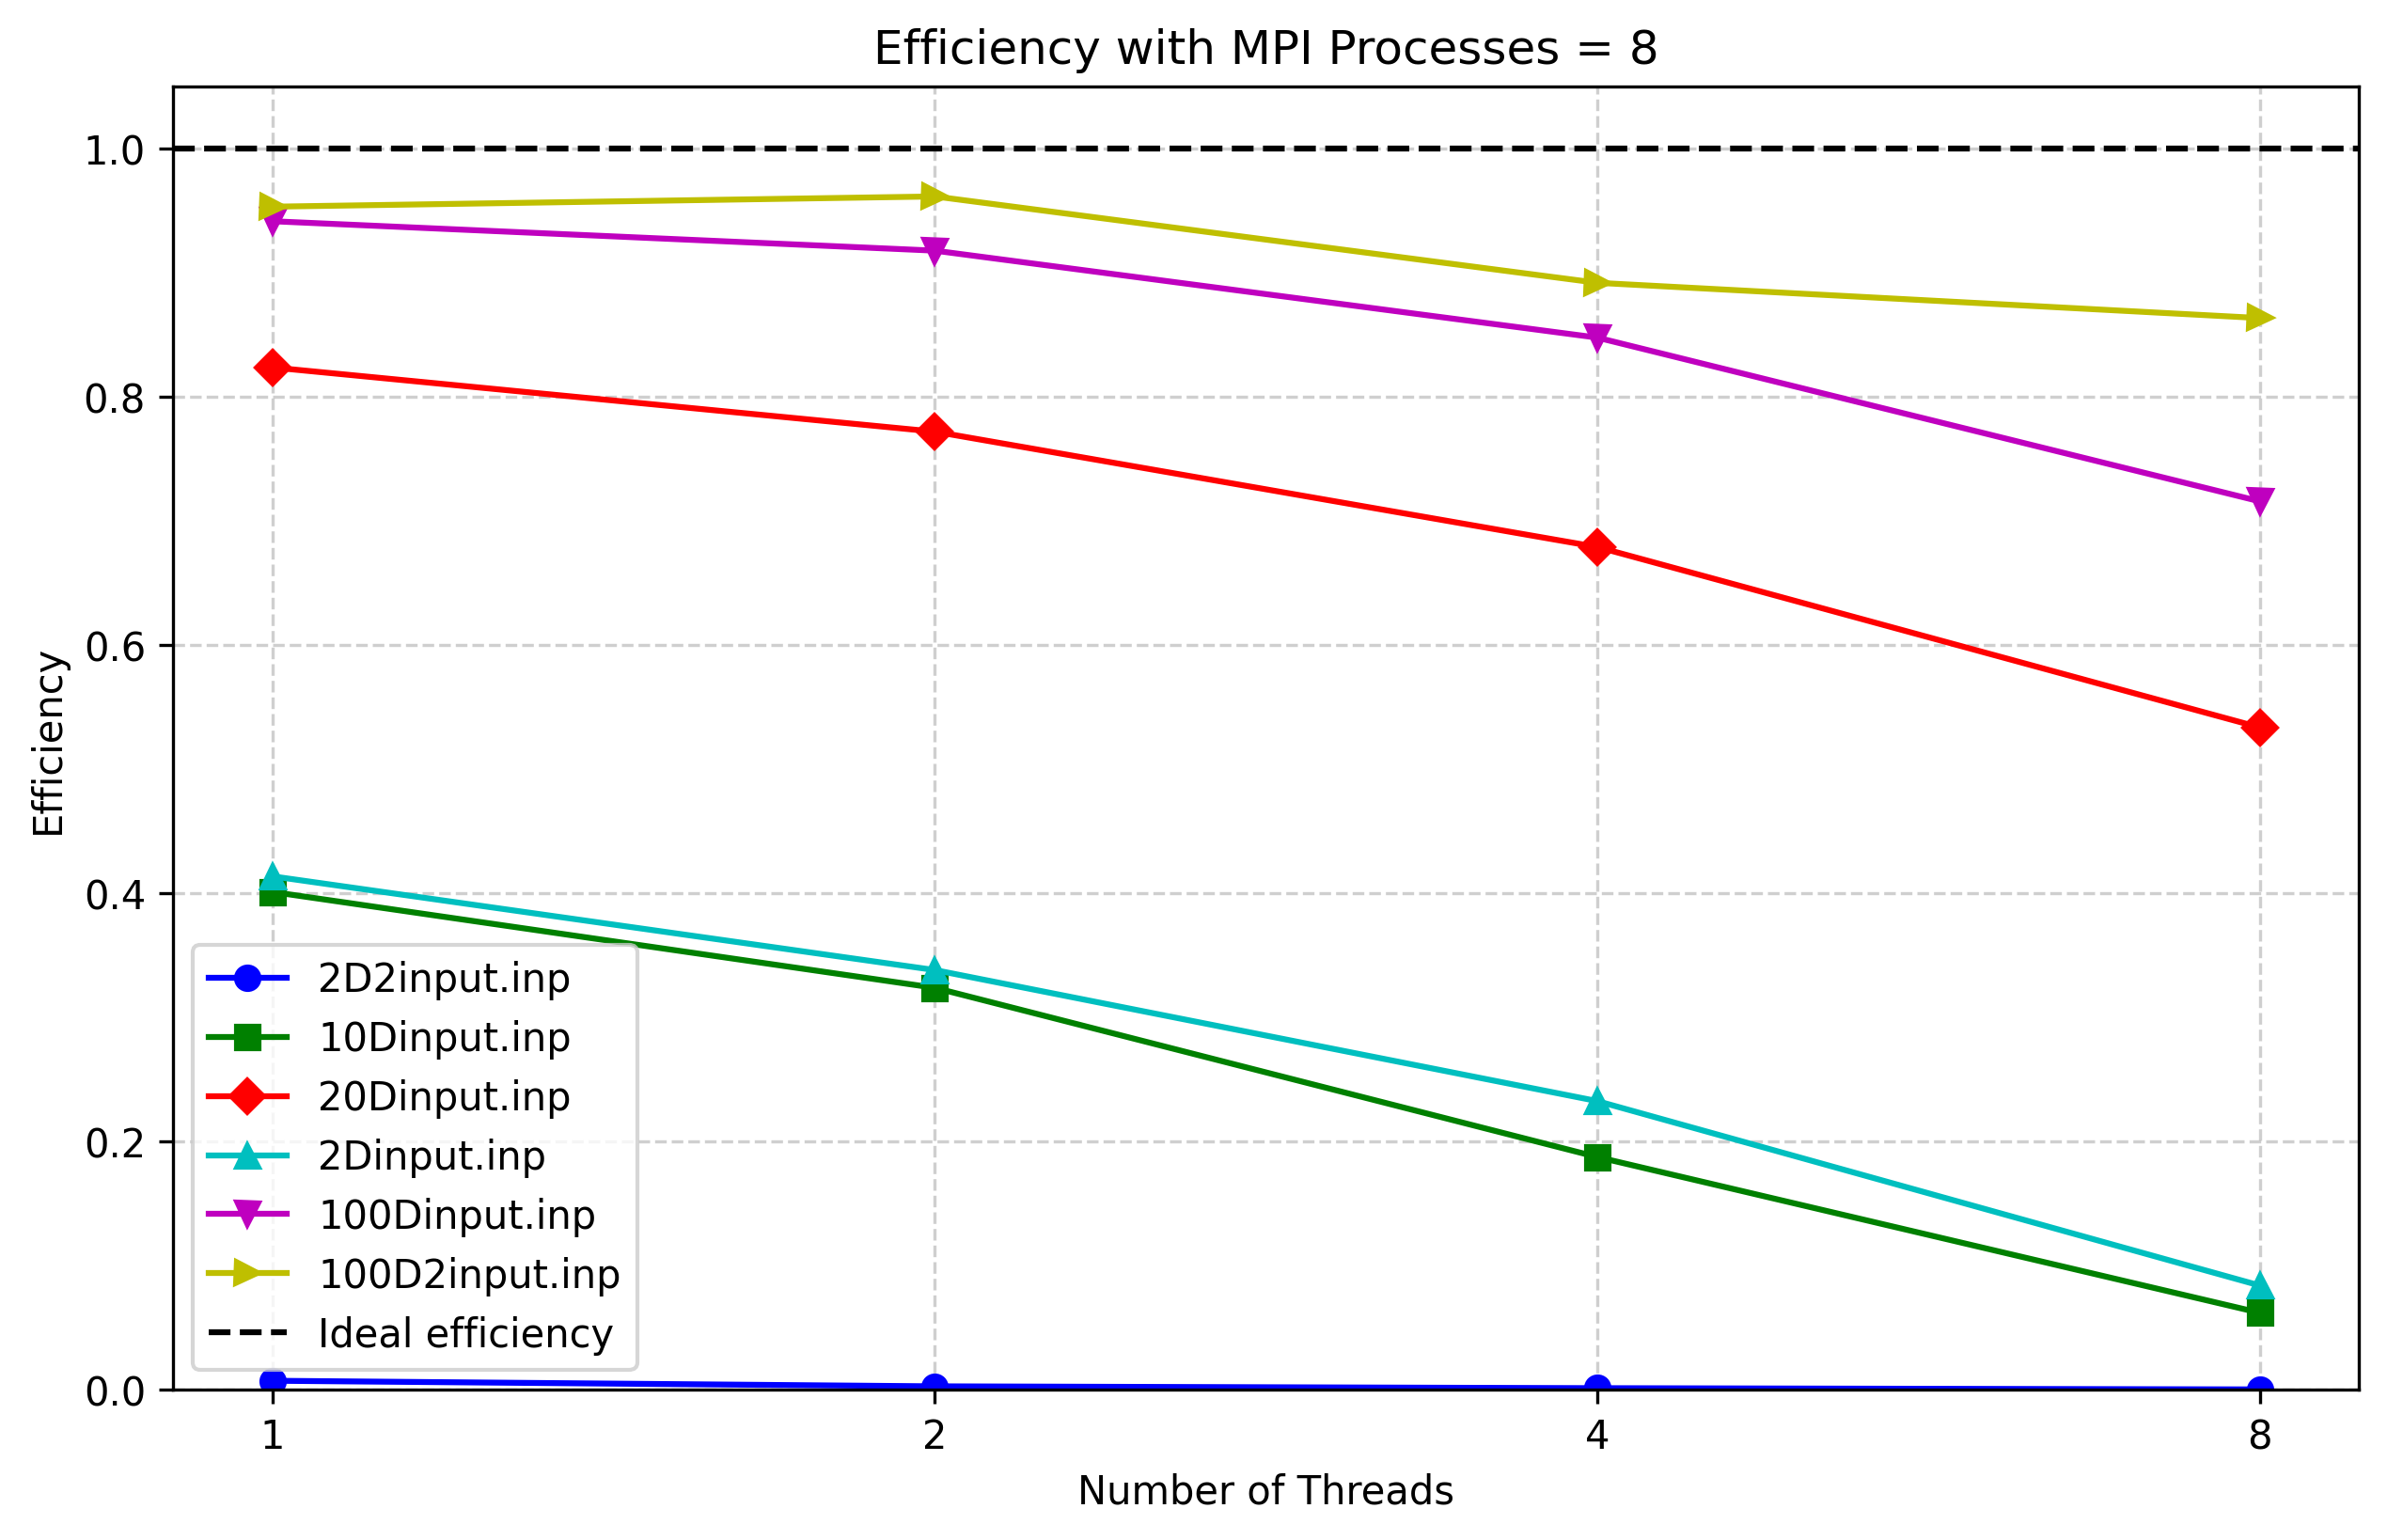
\includegraphics[width=\linewidth]{../test_csv/plots/efficency/plot_omp_mpi_8_small_slurm.png}
    \end{minipage}
    \begin{minipage}{0.4\textwidth}
      \centering
      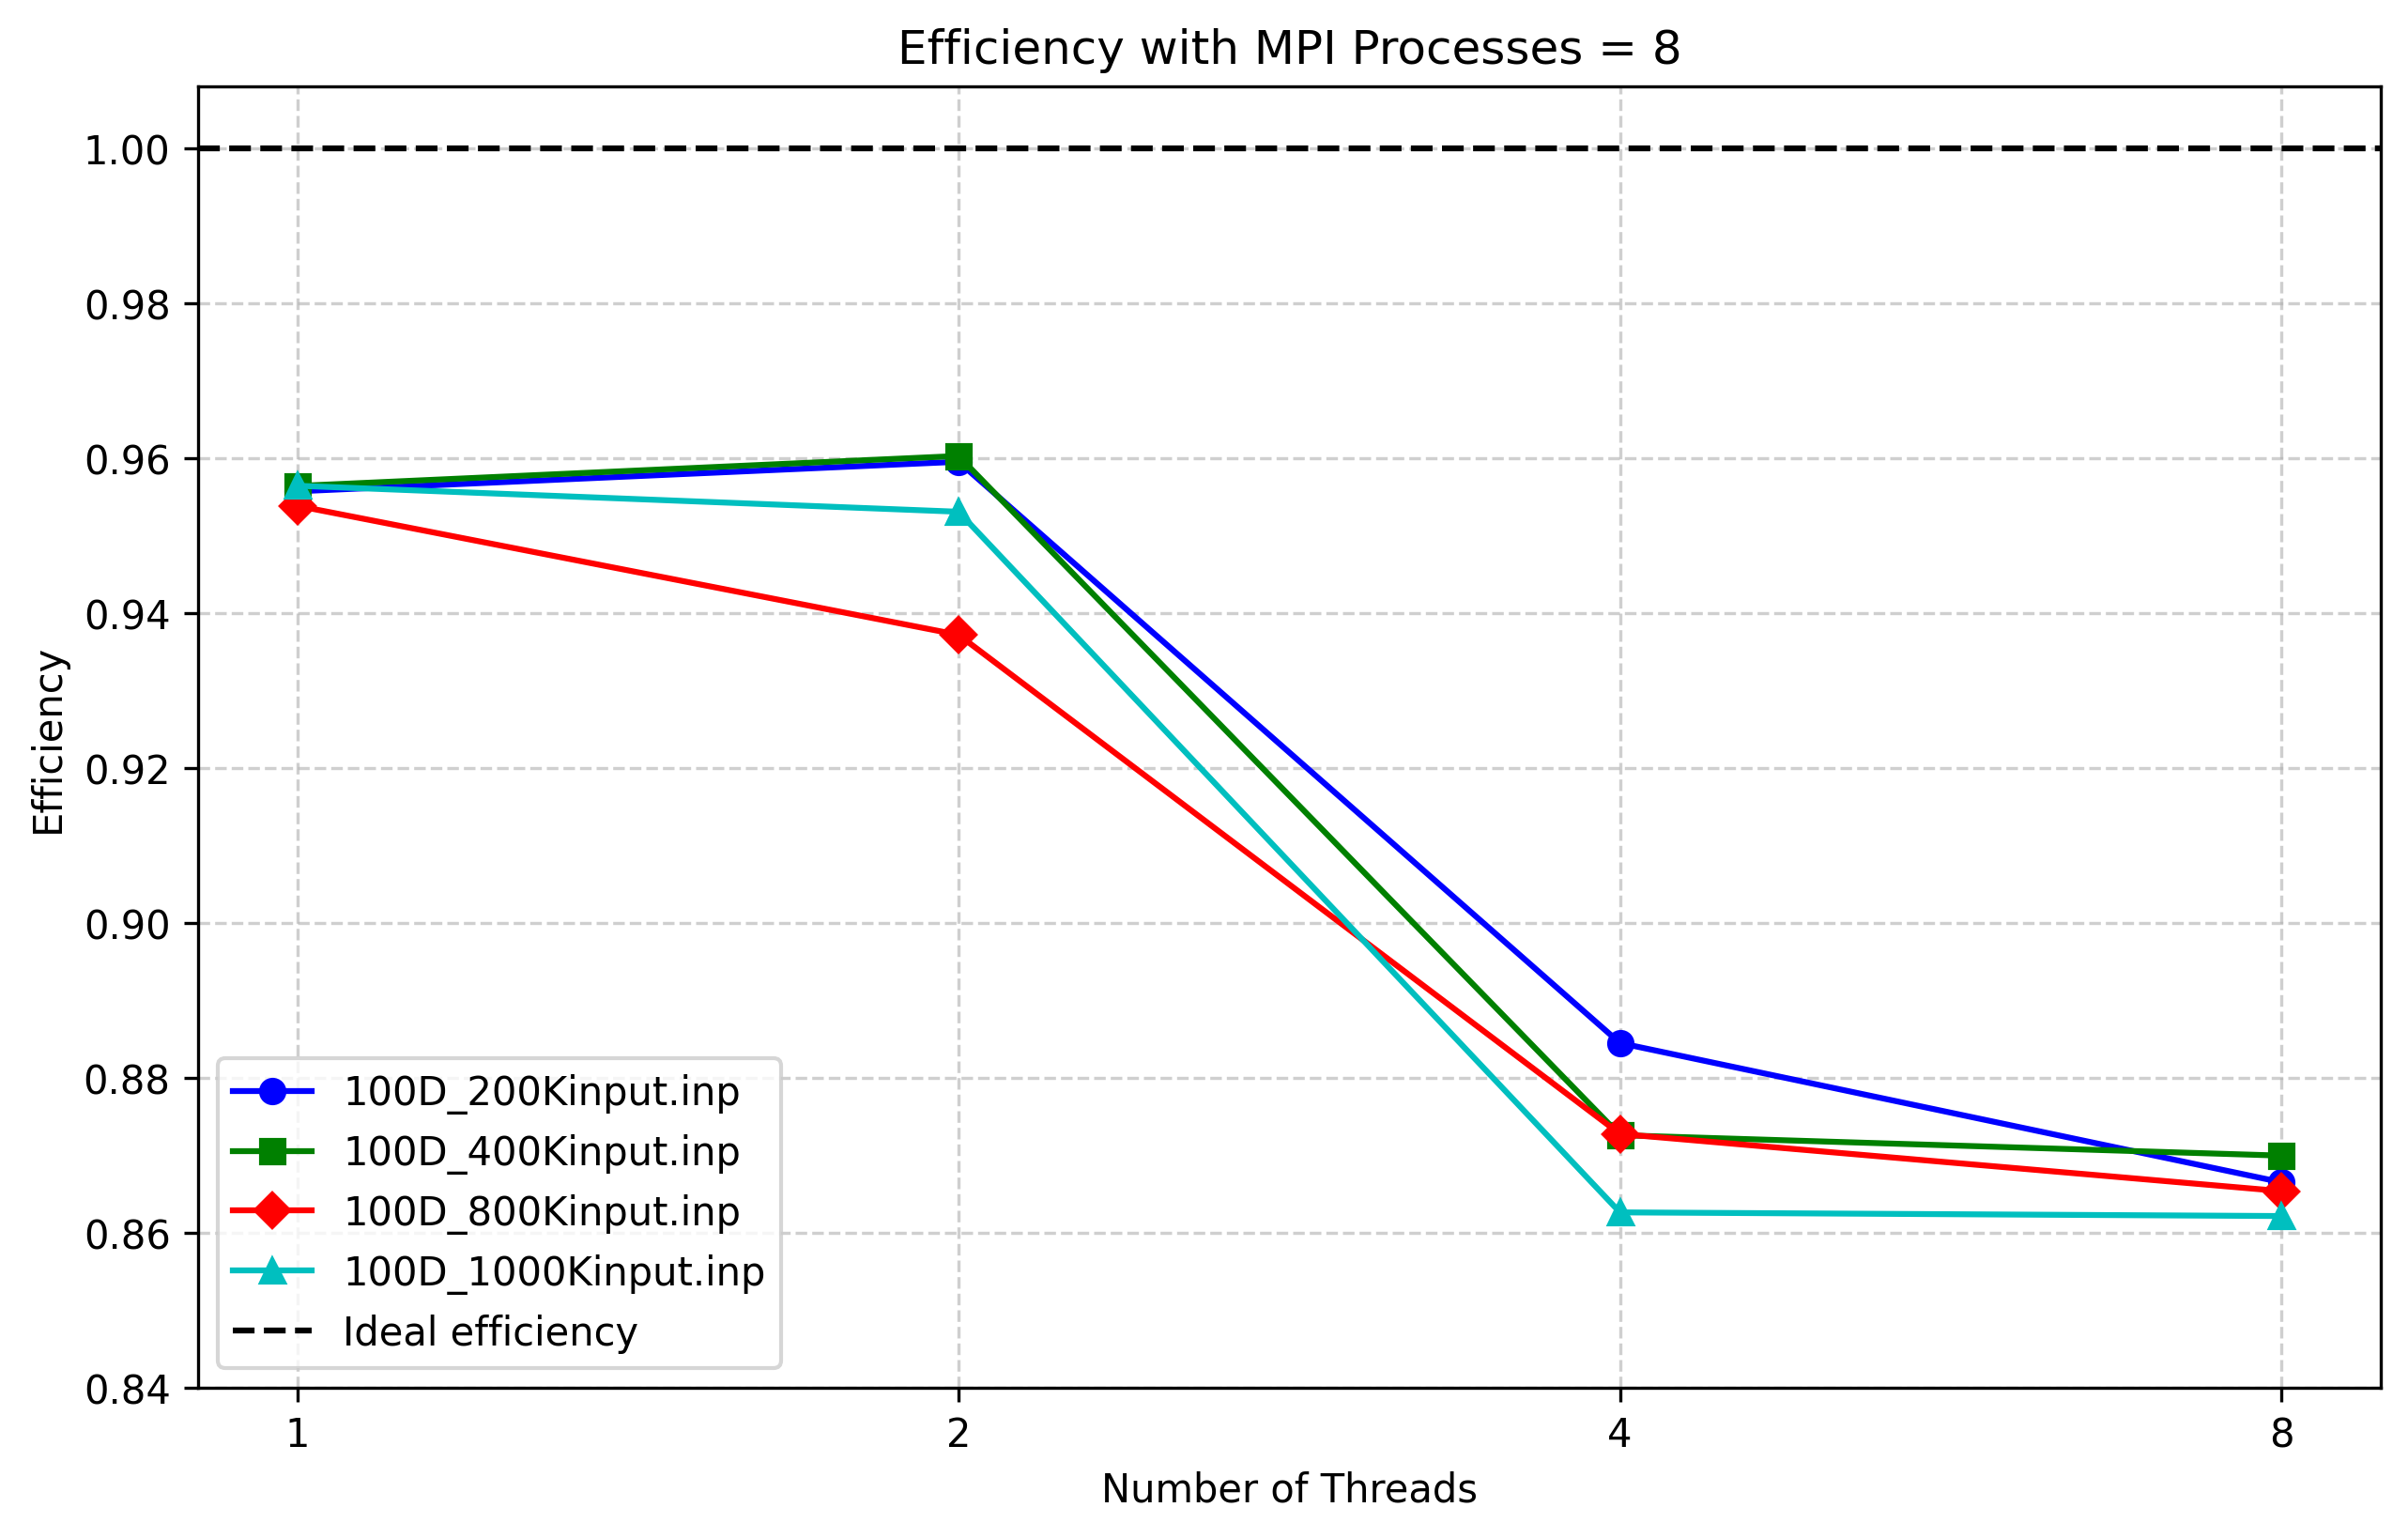
\includegraphics[width=\linewidth]{../test_csv/plots/efficency/plot_omp_mpi_8_big_slurm.png}
    \end{minipage}
  \end{figure}

  Con 8 processi notiamo che per i test grandi sia lo speedup che l'efficenza all'aumentare dei thread rimangono alti, mentre con i file input più leggeri, confrontando 
  con gli altri processi, sia lo speedup che l'efficenza sono basse all'aumentare del numero di thread, questo causato dalla concorrenza tra i thread. 

  In conclusione possiamo notare che l'efficenza e lo speedup nei test file più leggeri sono lontanti dal valore ideale, in quanto avendo pochi dati da elaborare si ha un overhead di comunicazione tra i vari processi e thread molto alto, influendo sull'esecuzione del programma. 
  Mentre nei test file più pesanti, lo speedup e l'efficenza mantengono dei buoni valori, alcuni molto vicini al valore ideale, sopratutto per quanto riguarda lo speedup, in quanto nei test più pesanti ha un valore molto vicino a quello ideale (che cambia in 
  base alle unità di calcolo utilizzate), infatti, in certi casi il programma ha quasi \textbf{speedup lineare}, lo notiamo con i test sul file 1000K su tutti i processi con 1, 2 e 4 thread. Un'atra caratteristica che possiamo notare è che andando ad aumentare le unità di calcolo, l'efficenza sui test pesanti 
  inzia a calare, nonstante questo mantiene dei valori molto buoni.

  \begin{center}
    \rule{2.5cm}{1pt} \makebox{\texttt{Time distribution, median and avarage}} \rule{2.5cm}{1pt}
  \end{center}

  Di seguito sono riportati i graifici della distribuzione dei tempi con cui sono stati calcolati gli speedup e l'efficenza di ogni processo, in particolare sono riportati i grafici 
  con i processi utilizzando 8 thread per ogni processo.
  \begin{enumerate}
    \item Time distribution con 2 processi [\ref{time_d_2_small}] [\ref{time_d_2_big}]
    \item Time distribution con 4 processi [\ref{time_d_4_small}] [\ref{time_d_4_big}]
    \item Time distribution con 8 processi [\ref{time_d_8_small}] [\ref{time_d_8_big}]
  \end{enumerate}

  Per ogni processo possiamo notare che la mediana e la media nel grafico con file input 1000K sono molto vicini tra loro, indicando una simmetria dei dati, di conseguenza non vi è troppo distacco 
  di tempo tra i vari test, lo possiamo notare anche dal \textbf{coefficente di variazione} che essendo molto basso indica che i tempi sono molto stabili 
  e non hanno troppe variazioni tra di loro. Tuttavia, notiamo che nel grafico con il file input 2D2 la situazione è ben diversa, in quanto la mediana 
  e la media sono distanti e il CV è molto alto, indicando che i tempi non sono molto stabili e poco prevedibili, molto probabilmente
  questo è dovuto al fatto che il programma sul file input 2D2 riscontra problemi di overhead di comunicazione tra processi, e anche un minimo ritardo da parte di 
  un processo nella comunicazione influisce molto sul tempo di esecuzione.

  \begin{figure}[ht]
    \centering
    \begin{minipage}{0.45\textwidth}
      \centering
      \caption{\textbf{Time distribution 2 process s.}}
      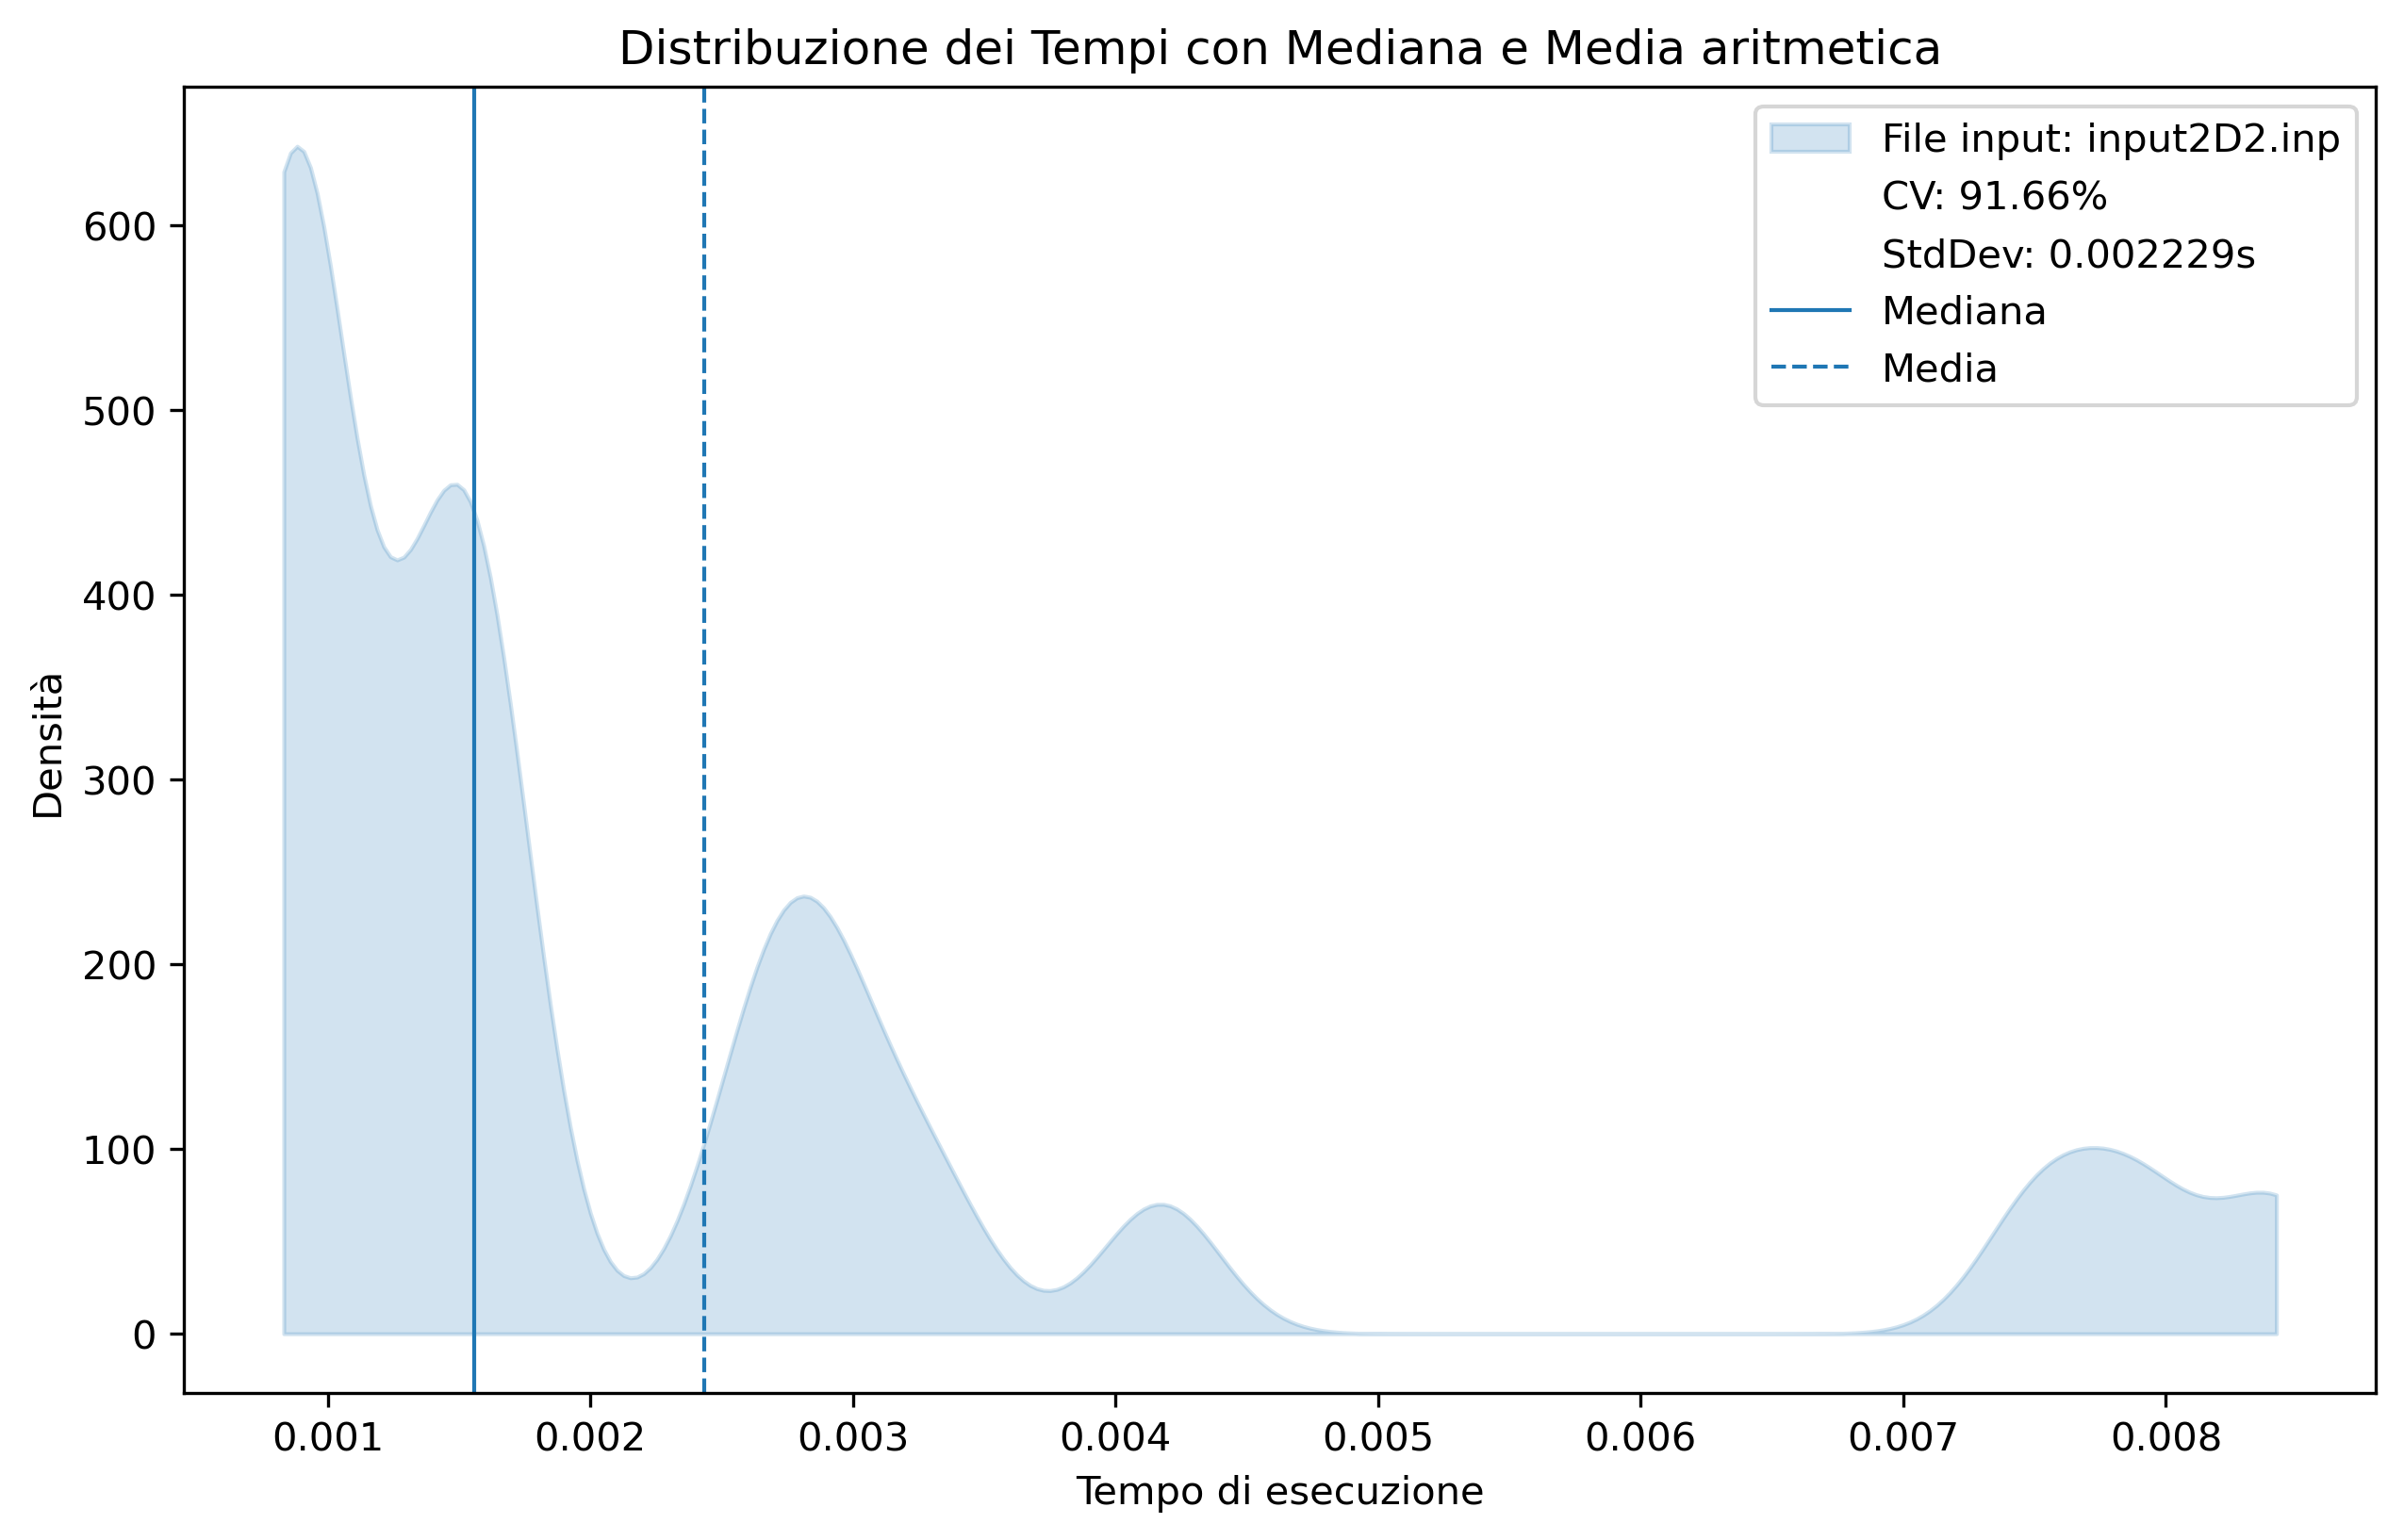
\includegraphics[width=\linewidth]{../test_csv/plots/time_distribution/time_distribution_2D2_omp_mpi_2.png}
      \label{time_d_2_small}
    \end{minipage}
    \begin{minipage}{0.45\textwidth}
      \centering
      \caption{\textbf{Time distribution 2 process b.}}
      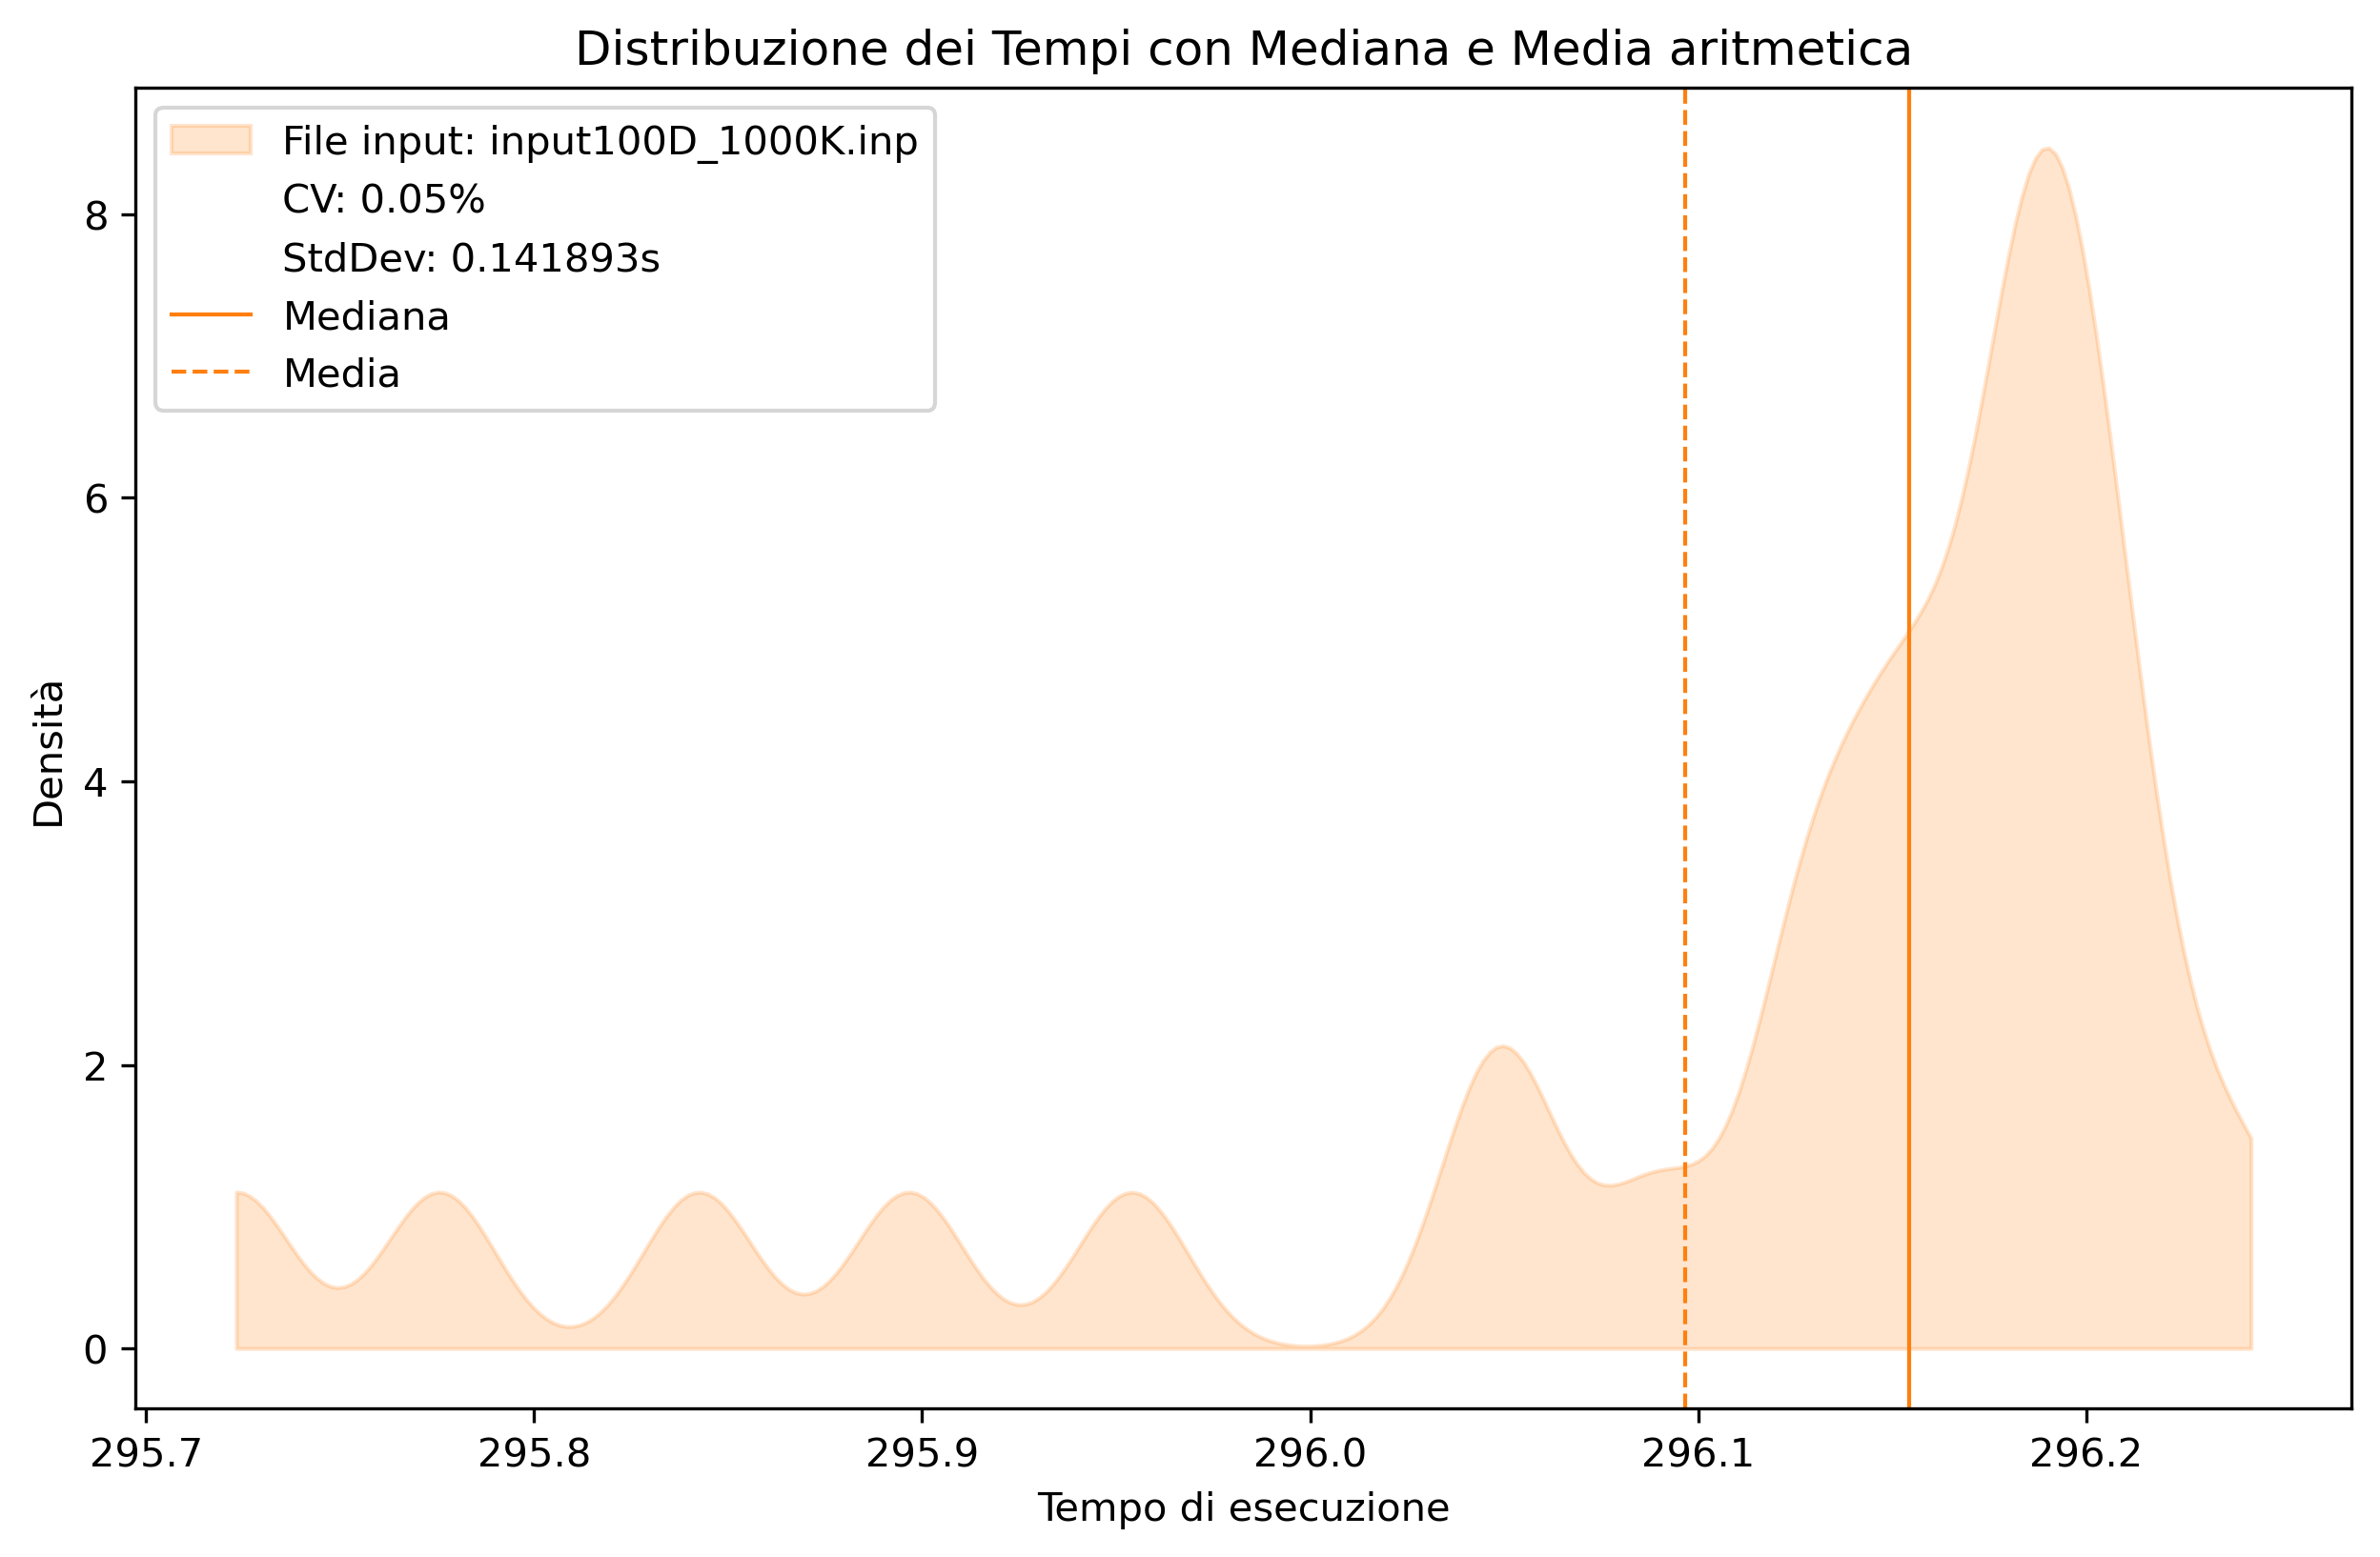
\includegraphics[width=\linewidth]{../test_csv/plots/time_distribution/time_distribution_100D_1000K_omp_mpi_2.png}
      \label{time_d_2_big}
    \end{minipage}
    \begin{minipage}{0.45\textwidth}
      \centering
      \caption{\textbf{Time distribution 4 process s.}}
      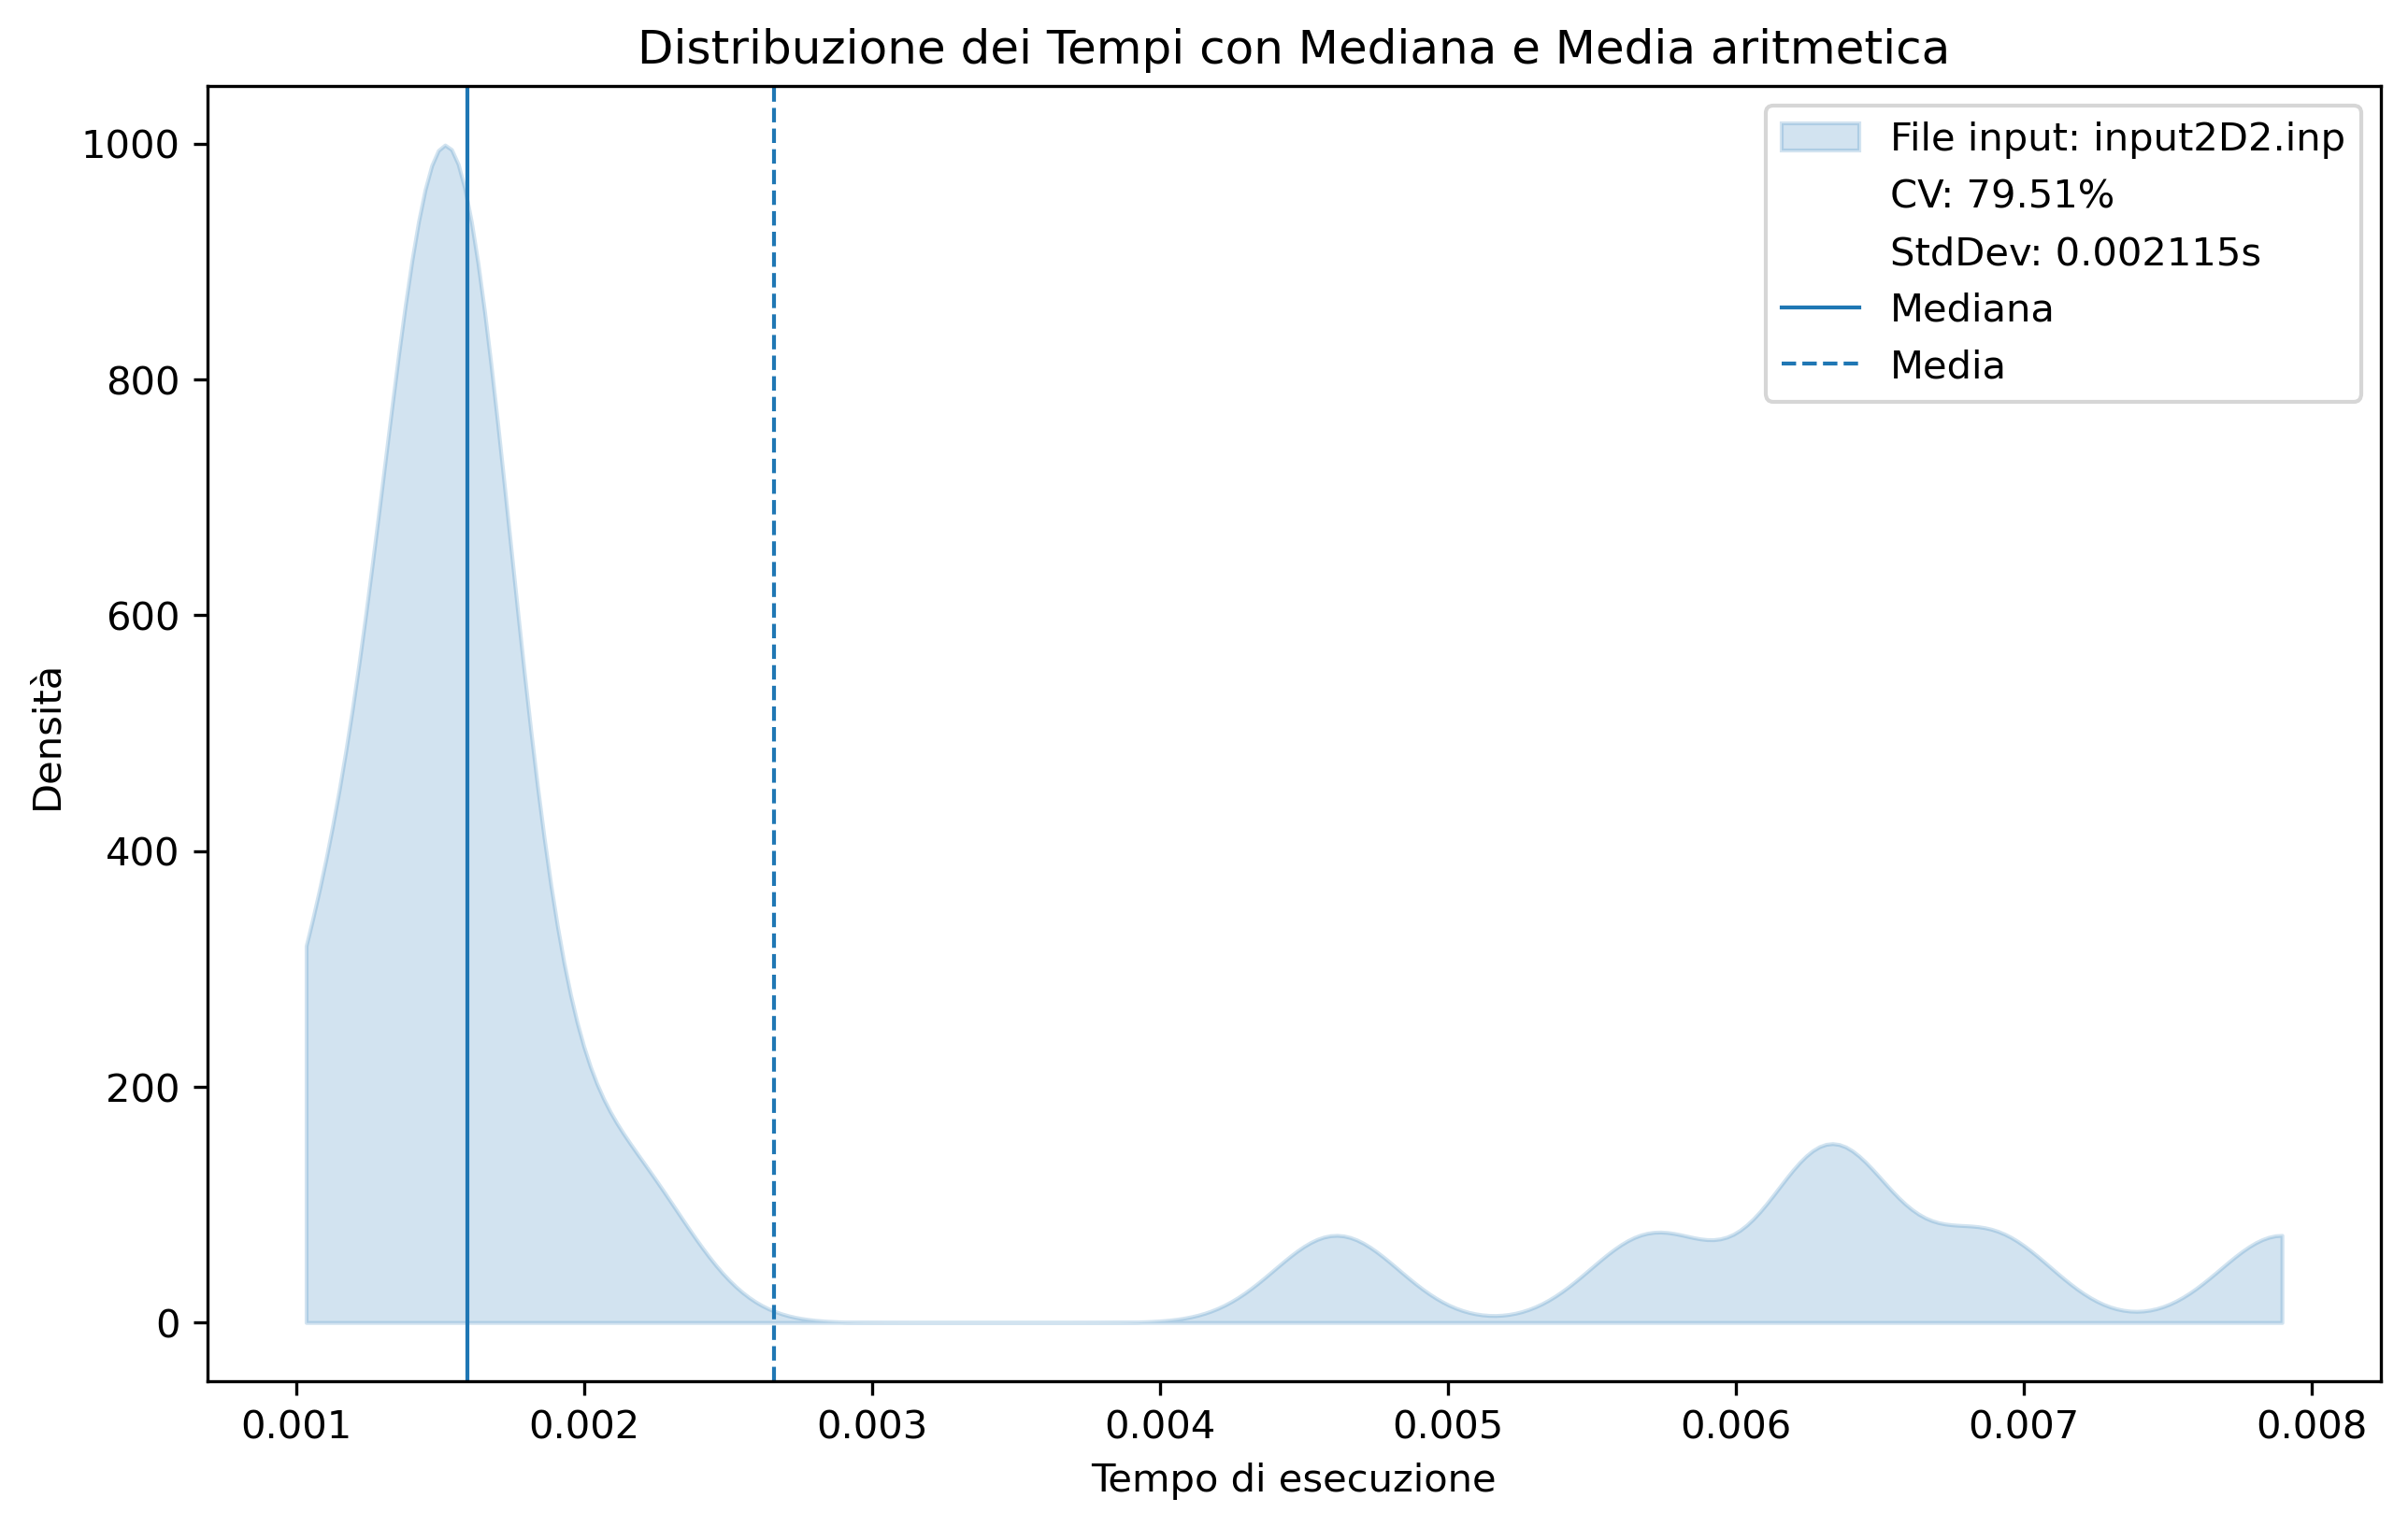
\includegraphics[width=\linewidth]{../test_csv/plots/time_distribution/time_distribution_2D2_omp_mpi_4.png}
      \label{time_d_4_small}
    \end{minipage}
    \begin{minipage}{0.45\textwidth}
      \centering
      \caption{\textbf{Time distribution 4 process b.}}
      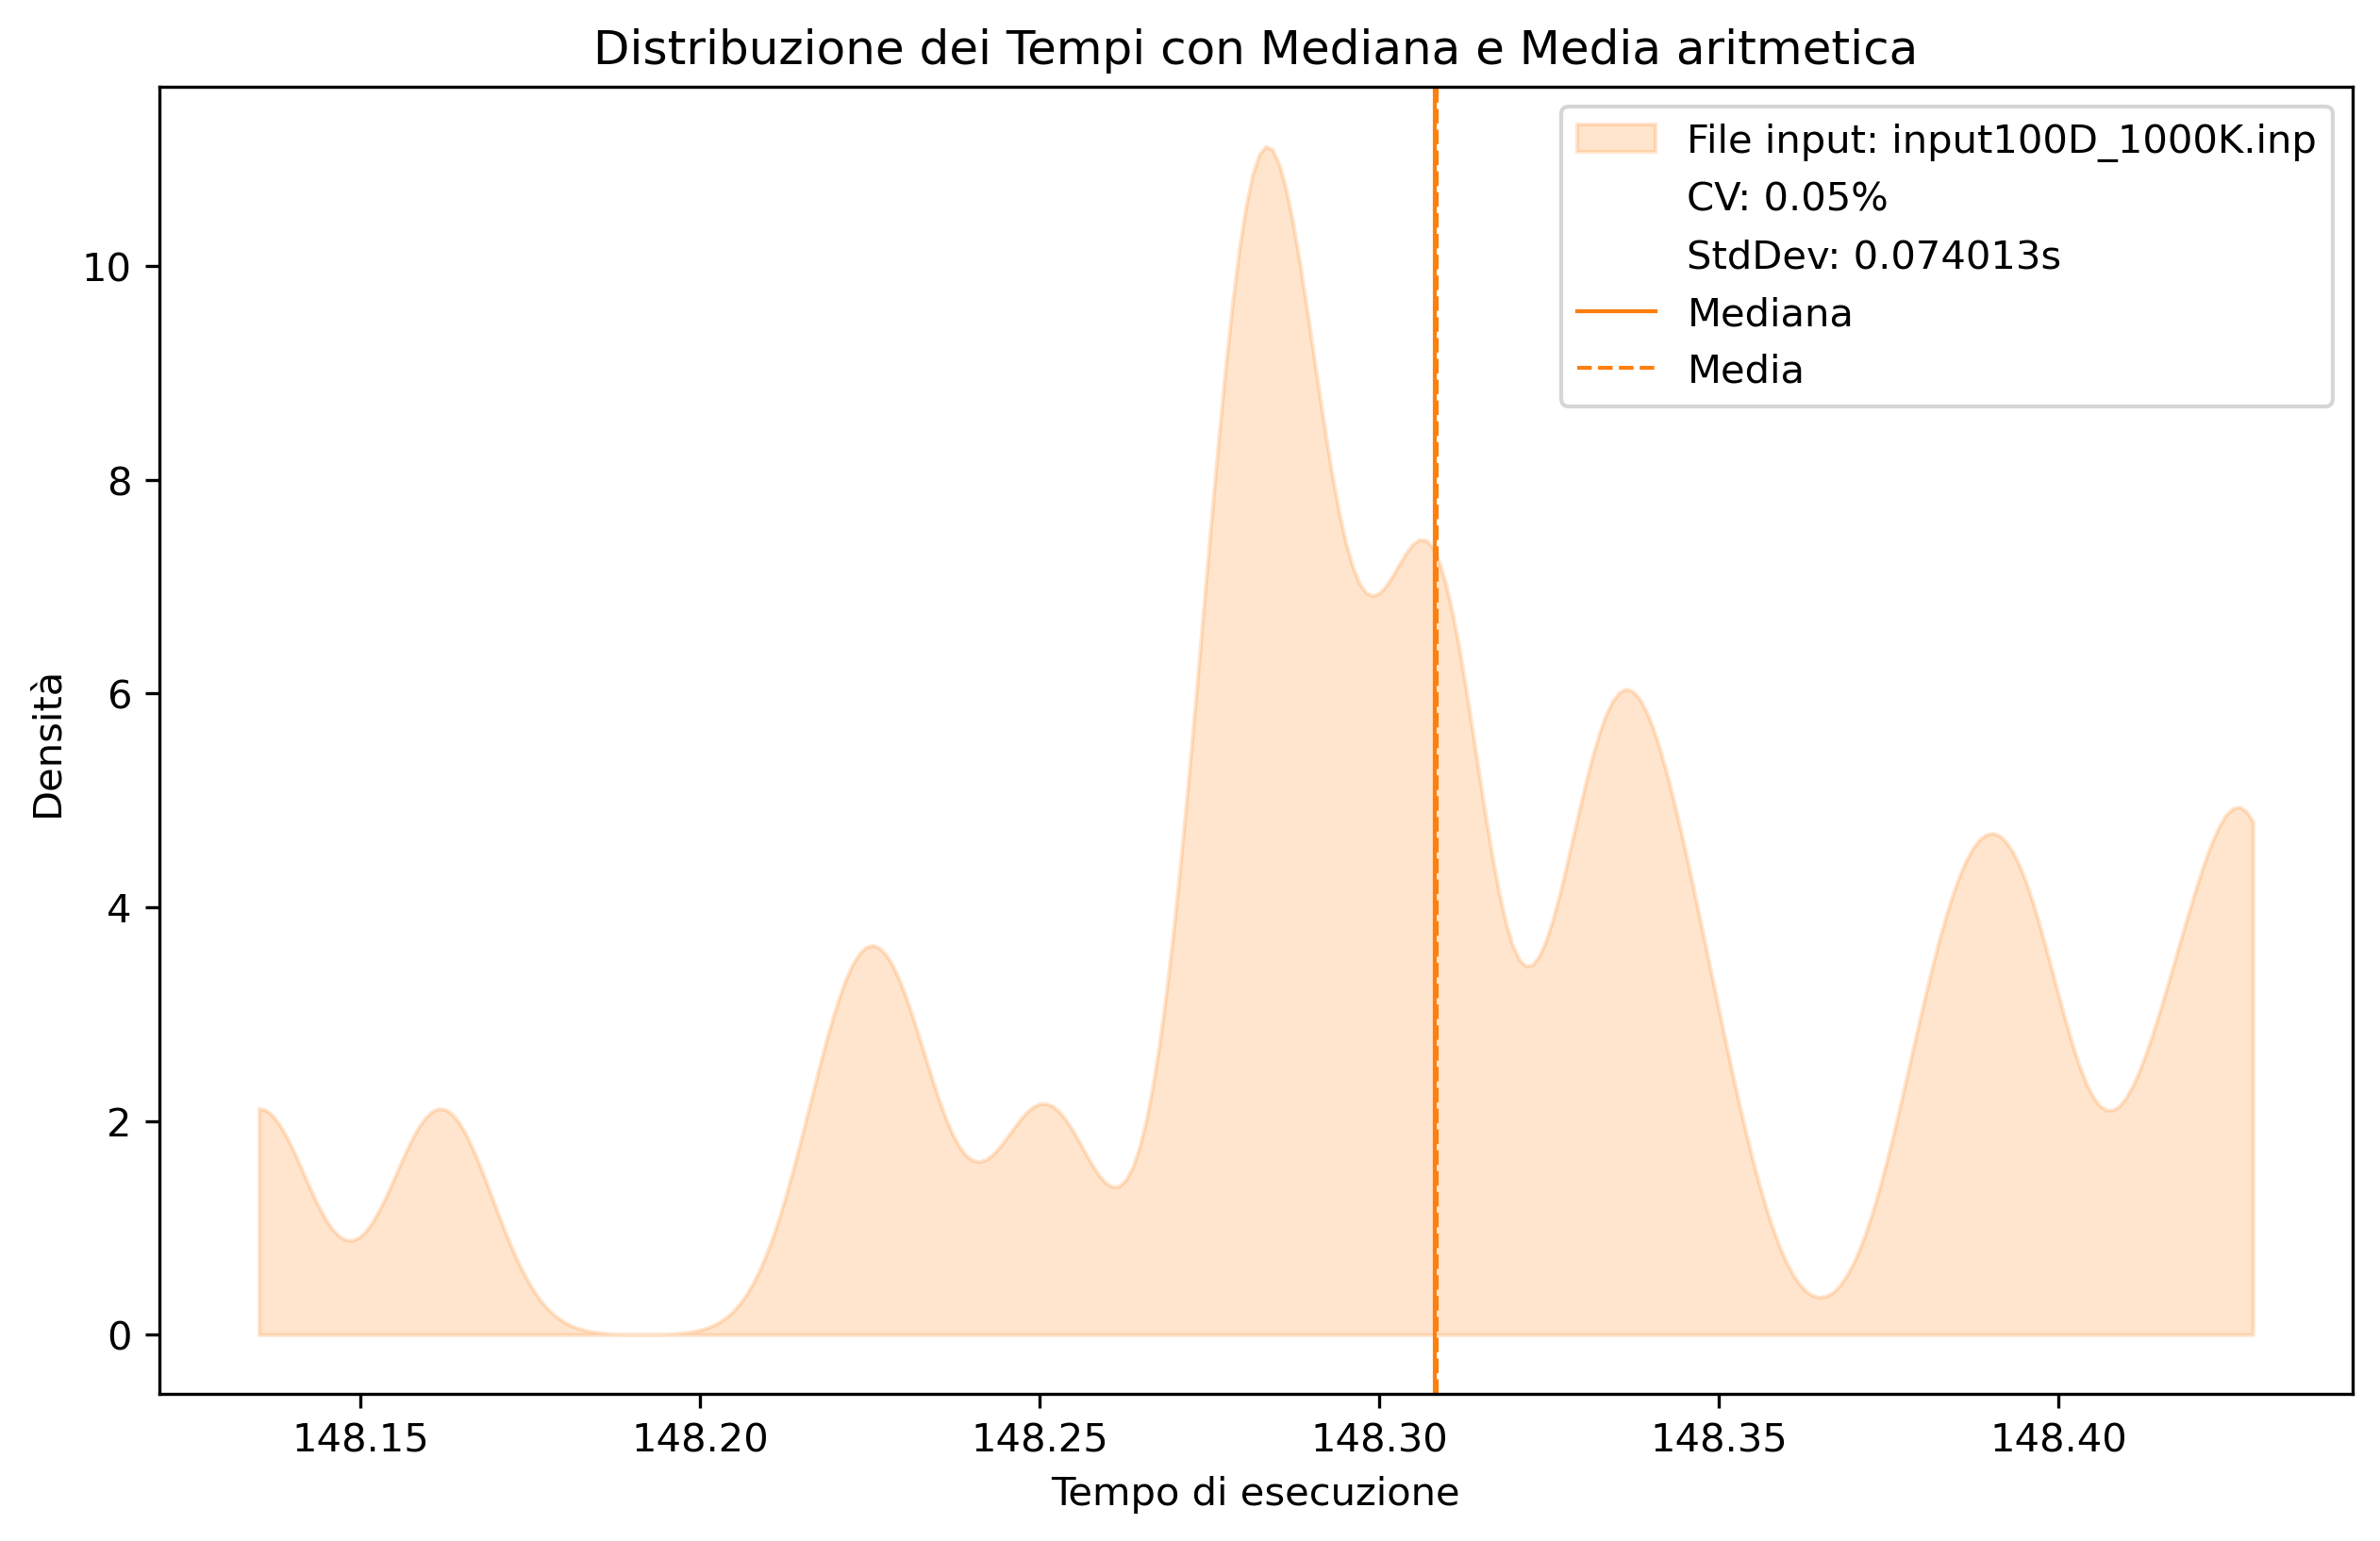
\includegraphics[width=\linewidth]{../test_csv/plots/time_distribution/time_distribution_100D_1000K_omp_mpi_4.png}
      \label{time_d_4_big}
    \end{minipage}
    \begin{minipage}{0.45\textwidth}
      \centering
      \caption{\textbf{Time distribution 8 process s.}}
      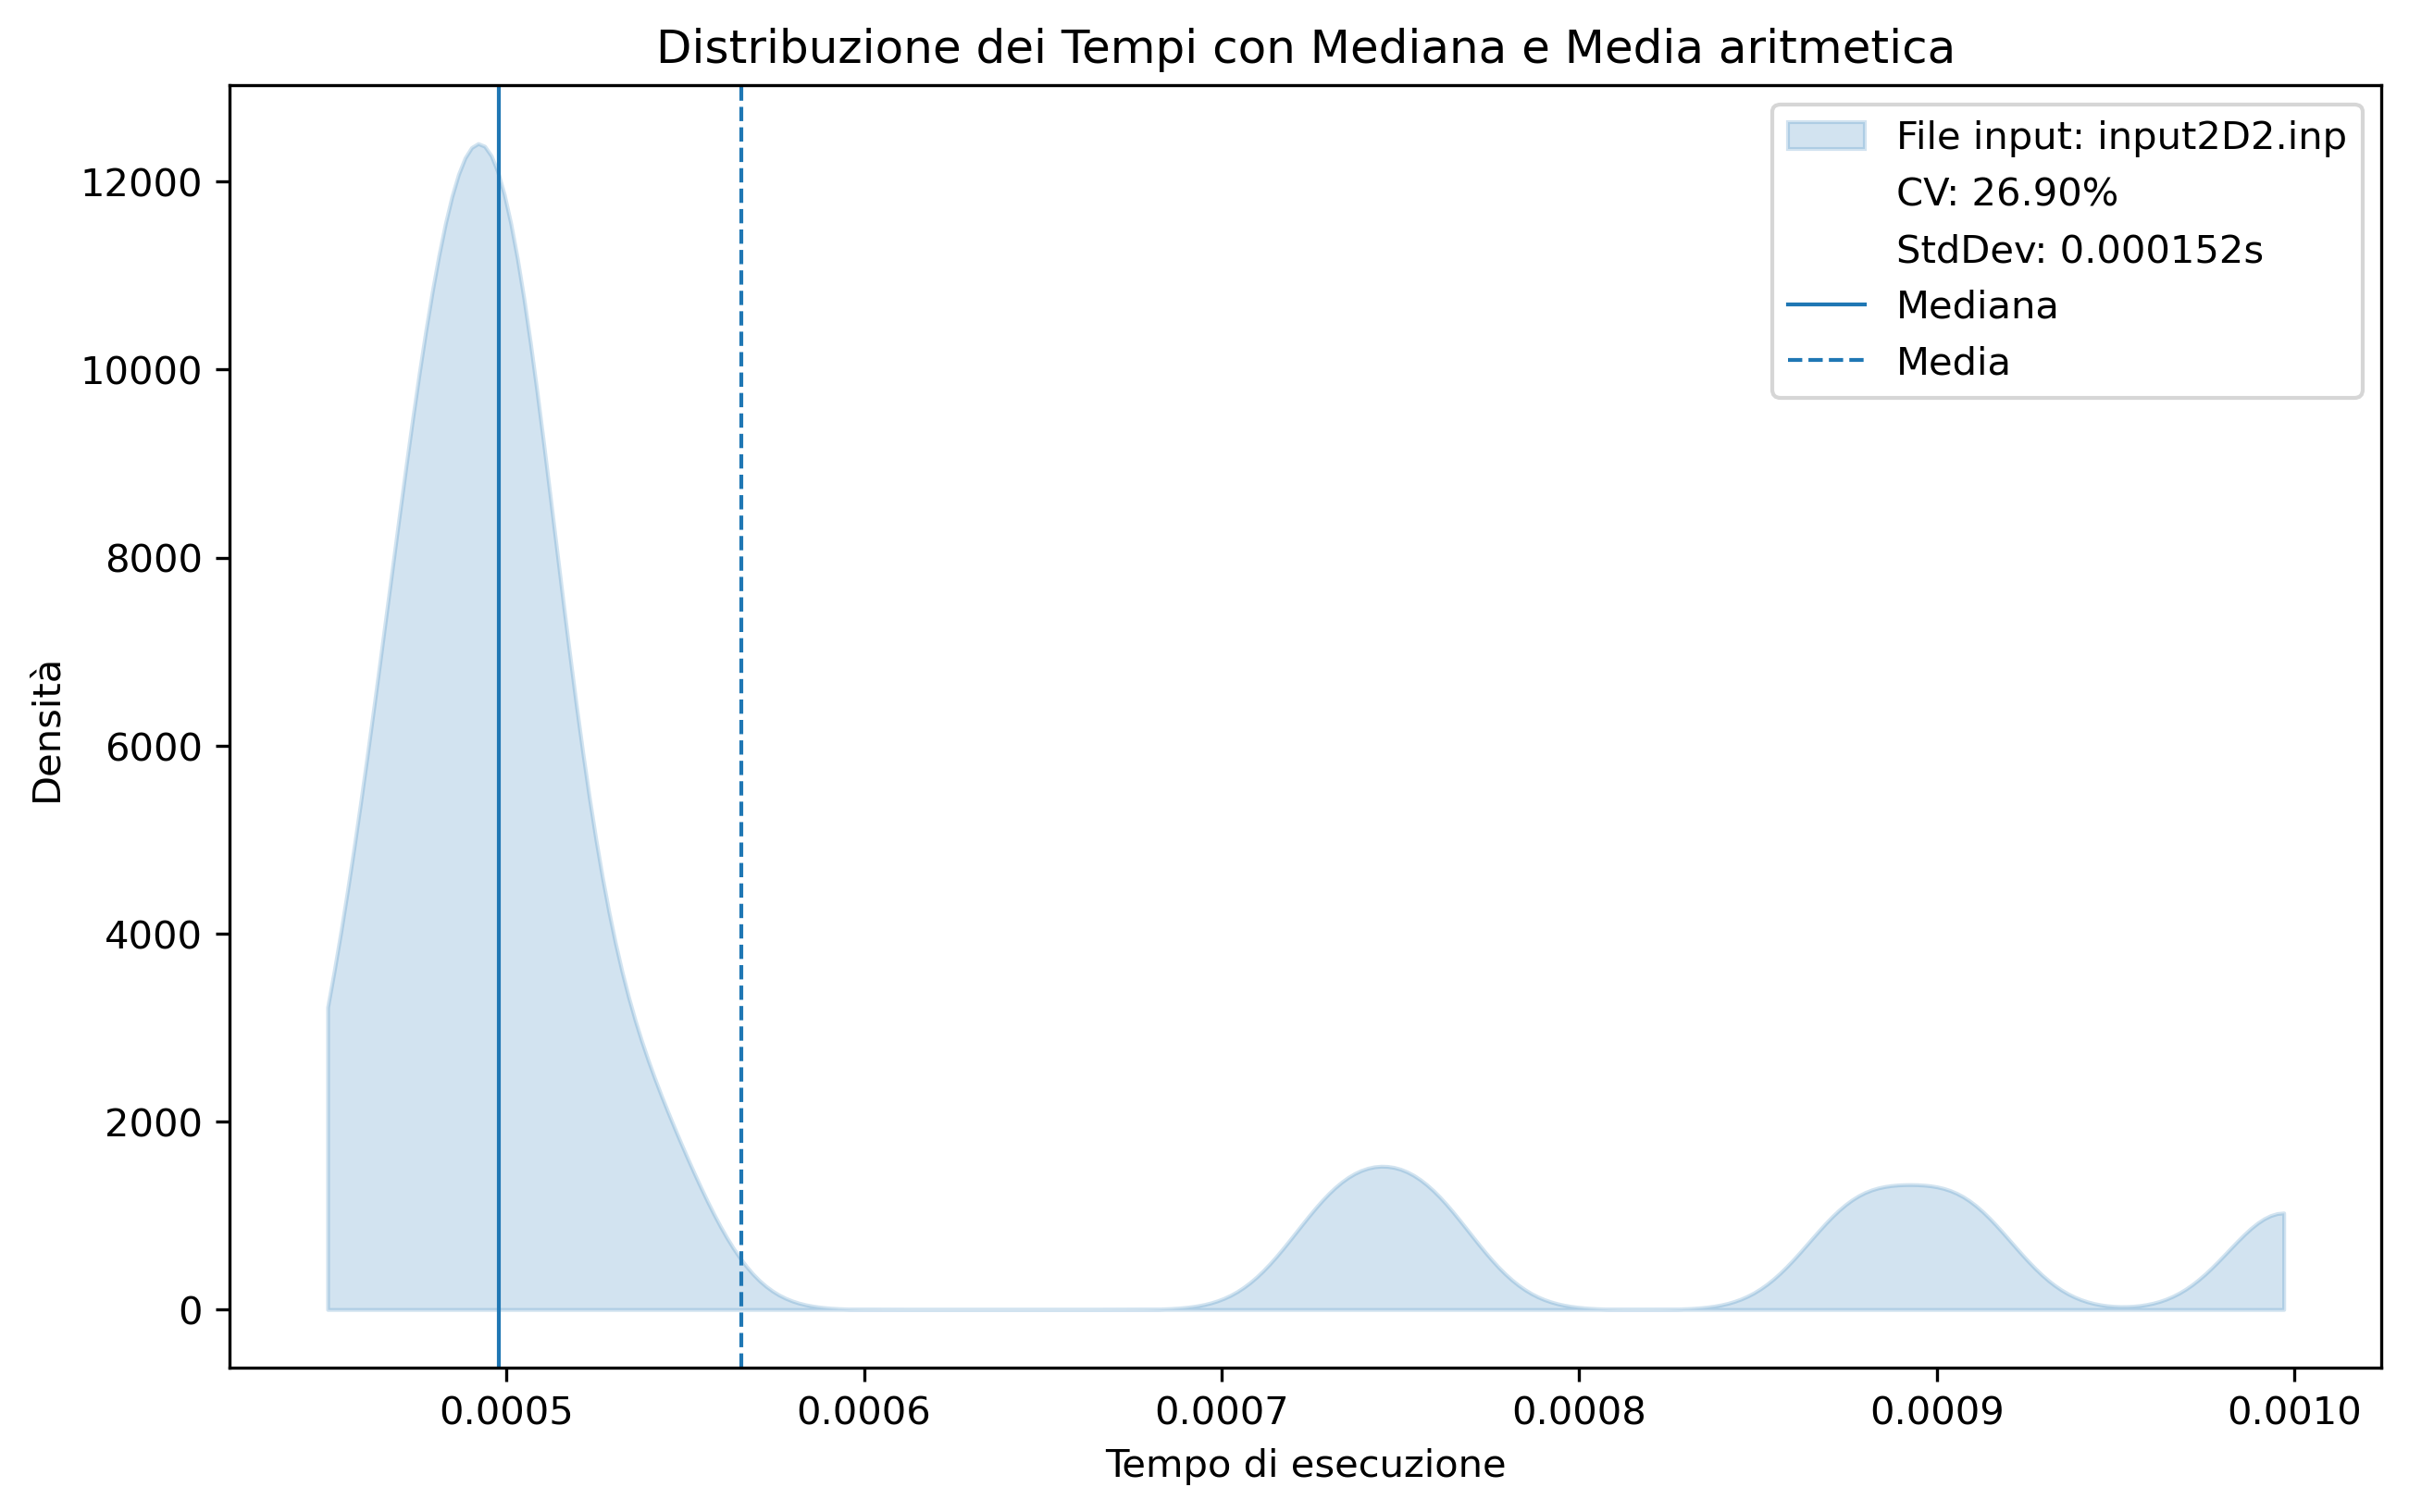
\includegraphics[width=\linewidth]{../test_csv/plots/time_distribution/time_distribution_2D2_omp_mpi_8.png}
      \label{time_d_8_small}
    \end{minipage}
    \begin{minipage}{0.45\textwidth}
      \centering
      \caption{\textbf{Time distribution 8 process b.}}
      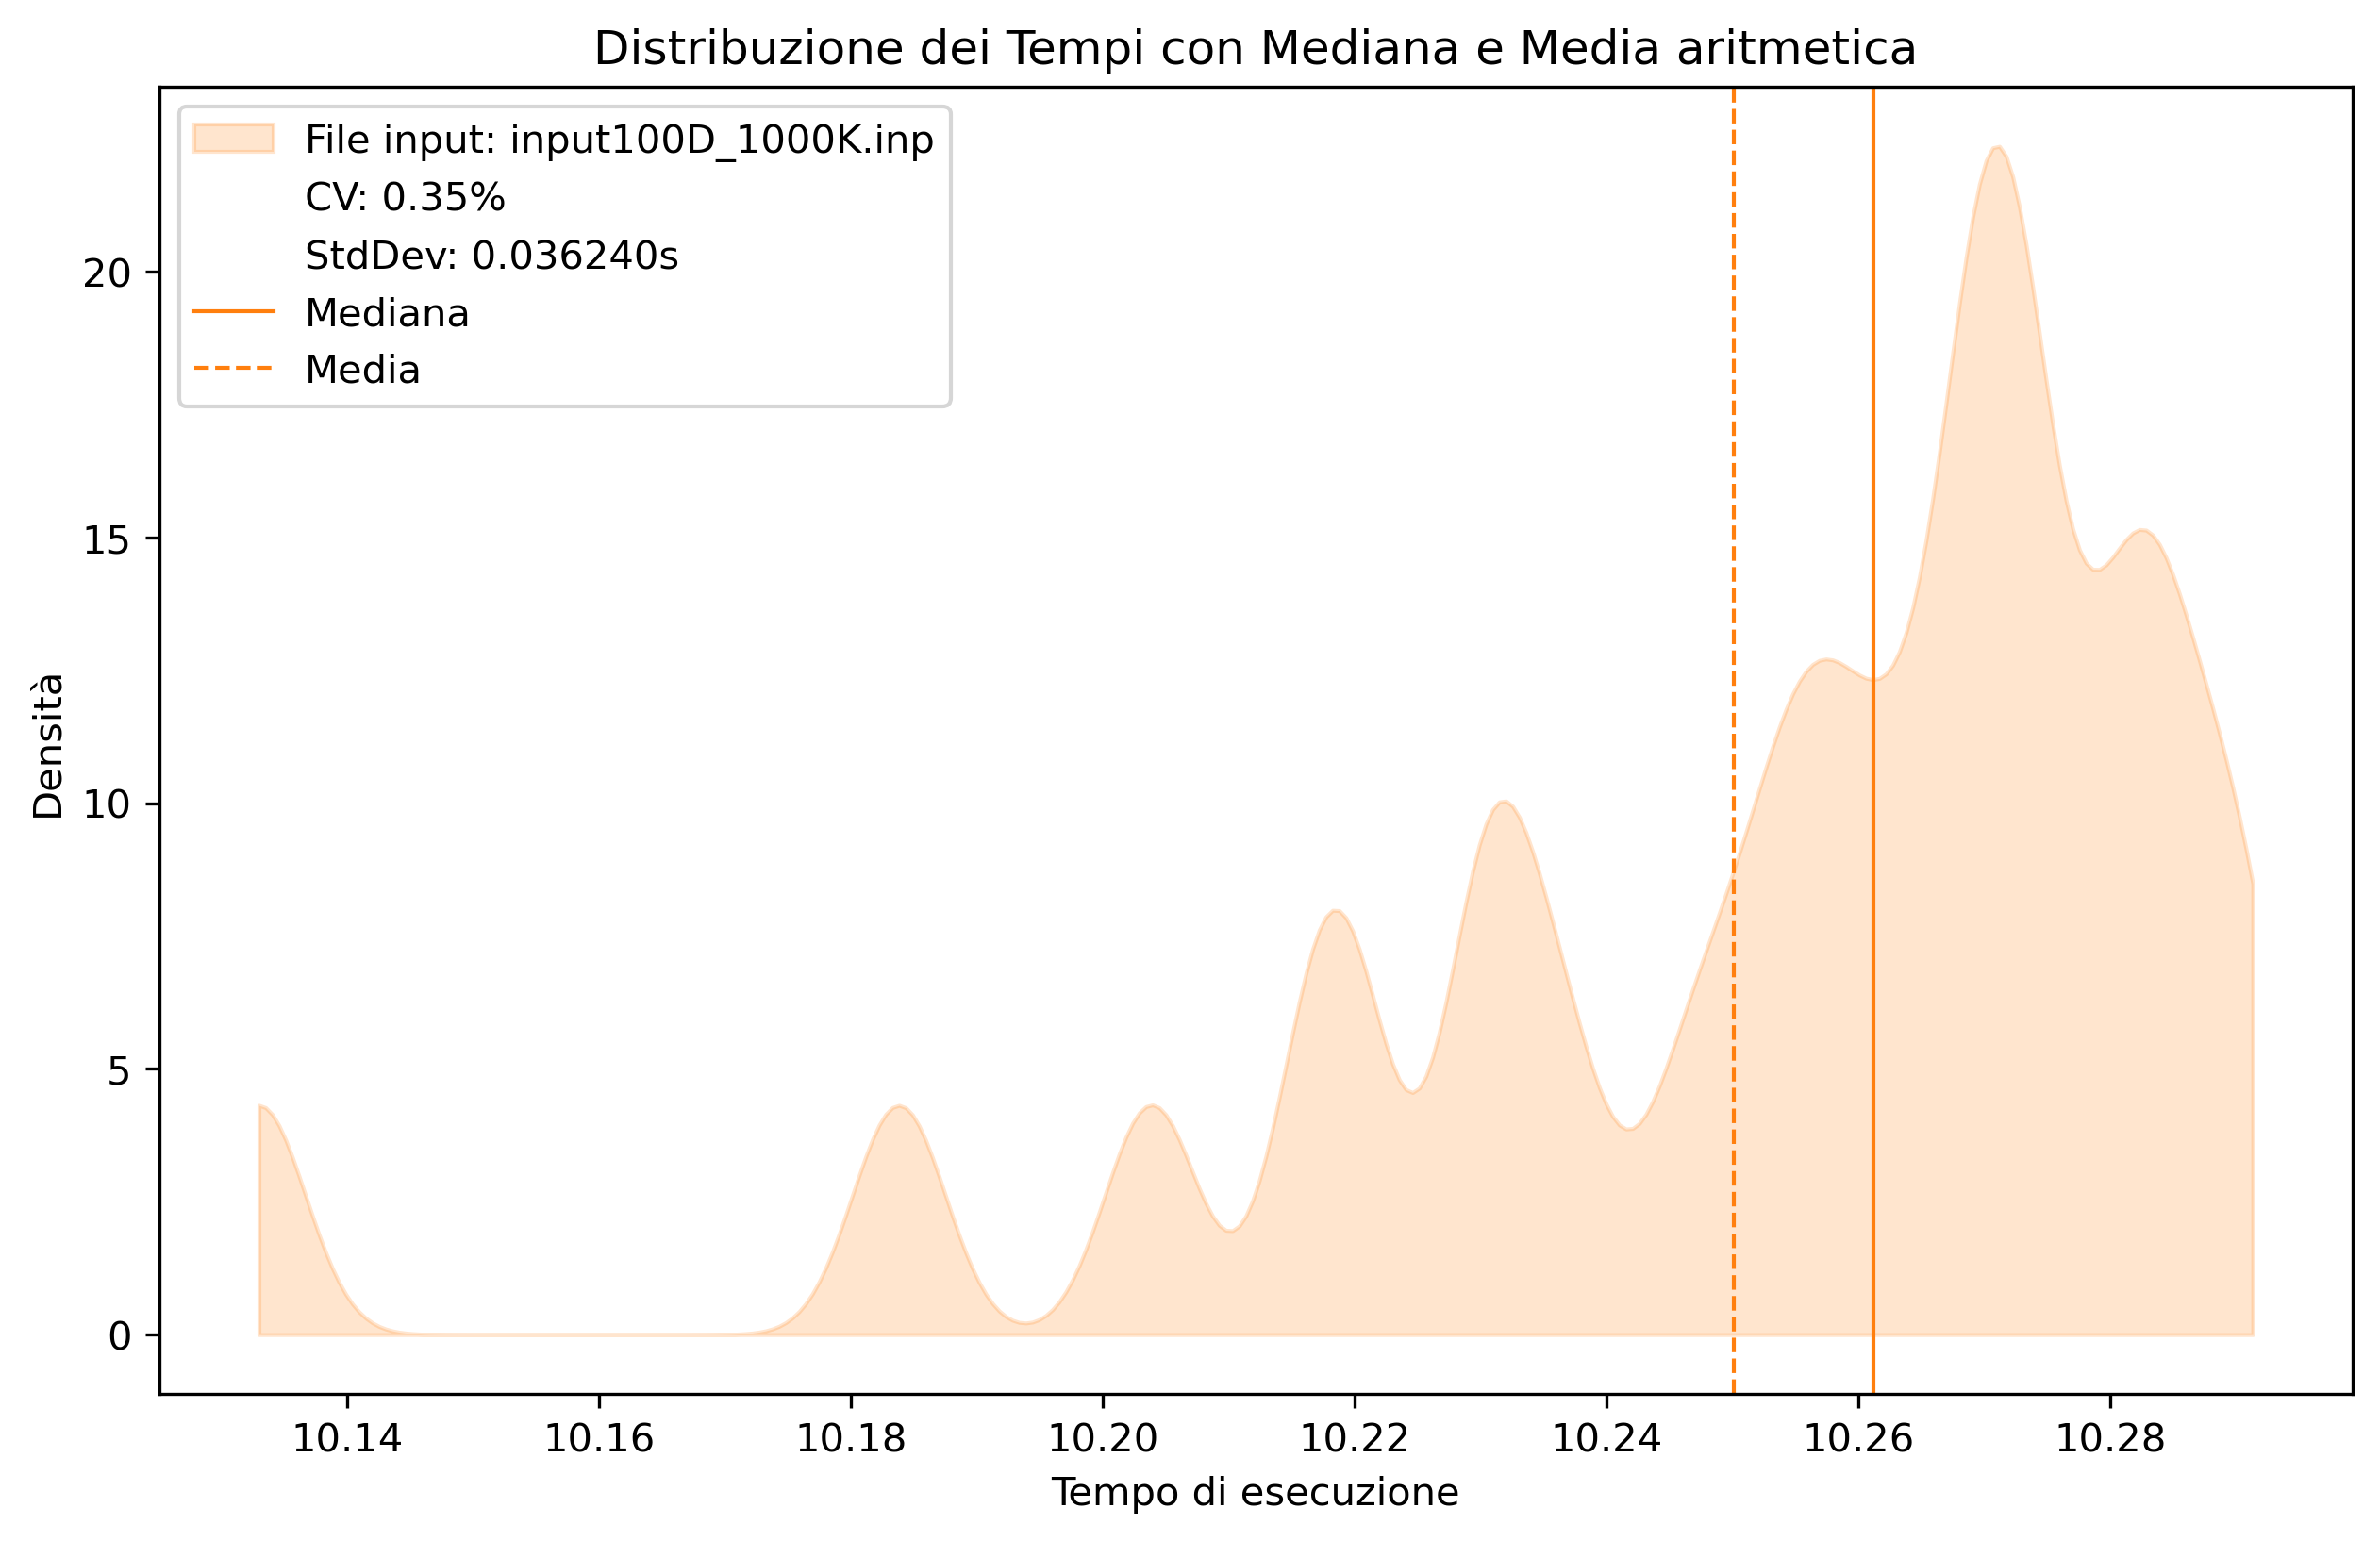
\includegraphics[width=\linewidth]{../test_csv/plots/time_distribution/time_distribution_100D_1000K_omp_mpi_8.png}
      \label{time_d_8_big}
    \end{minipage}
  \end{figure}

\end{document}
